\documentclass[12pt,a4paper, german]{article}
\usepackage[a4paper, left=2 cm, right=2 cm, top=2.5 cm, bottom=2 cm]{geometry}
\usepackage[T1]{fontenc}
\newcommand{\changefont}[3]{
\fontfamily{#1} \fontseries{#2} \fontshape{#3} \selectfont}
\usepackage[utf8]{inputenc}

\usepackage{wrapfig}
\usepackage{graphicx, subfigure}
\usepackage{float} 
\floatplacement{figure}{H}
%\usepackage{subcaption} 
\usepackage[format=hang,labelfont={bf,sf},font=small]{caption}  
\setlength{\captionmargin}{20pt} 

\usepackage{chngcntr}
\usepackage{amsfonts}  
\usepackage{amssymb}
\usepackage{amsmath}
\usepackage{verbatim}
\counterwithin{equation}{section}

\usepackage[numbers]{natbib}
\usepackage{babelbib}

%\usepackage{cite}

\usepackage[ngerman]{babel}

\setcounter{tocdepth}{4}   
\setcounter{secnumdepth}{4} 

\newcommand{\m}{ \ensuremath}
%opening
\title{Monte Carlo Simulation des Ising Modell}
\author{Niek Andresen, Robert Hartmann, Jan Fabian Schimd}
\date{WS 14/15}

\begin{document}
\begin{titlepage}
   

        \begin{center}
            \changefont{cmr}{m}{sc} 
            Institut für theoretische Physik\\
            der\\
            Universität Hamburg\\
            \vspace{5cm}

            \large\bf{Monte Carlo Simulation des Ising Modell}\\
           \vspace{2cm}       
             Computational Physics - Projekt\\\
            \vspace{3cm}
            \large Wintersemester 2014/15\\
	\vspace{2cm}
	Betreuer:\\
	Prof. Dr. Alexander Lichtenstein\\
	Jun.-Prof. Dr. Frank Lechermann\\
	



        \end{center}
\vfill
	\parbox{5cm}{\footnotesize
           Niek Andresen\\
           Matrikel-Nr.: ???\\
	Computing in Science}
\hfill
	\parbox{5cm}{\footnotesize
           Robert Hartmann\\
           Matrikel-Nr.: 6426119\\
	Computing in Science}
\hfill
	\parbox{5cm}{\footnotesize
           Jan Fabian Schmid\\
           Matrikel-Nr.: 6440383\\
	Computing in Science}
\end{titlepage}
\maketitle

\tableofcontents
\newpage

\section{Problemstellung und Theorie}
\subsection{Das Ising-Modell}

Das Ising-Modell beschreibt näherungsweise den Ferromagnetismus in Festkörpern. Hierbei wird ein Kristall als äquidistantes Gitter gesehen, an dessen Gitterpunkten sich einzelne Spins befinden, welche ein magnetisches Moment haben. In der Näherung verändern sich die Positionen der Spins nicht. Nimmt man zusätzlich an, dass nur nächste Nachbarn im Gitter sich gegenseitig beeinflussen und beschränkt man nun noch die Spins in ihre z-Richtung und lässt sie nur zwei diskrete Werte annehmen ($\pm1$), ergibt sich der Hamiltonoperator:\\
\[
\hat{H}=-J\sum_{<i,j>} S_i S_j - B\sum_{i=1}^N S_i
\]
wobei $S_i \in \{-1,+1\}$. J ist die Kopplungskonstante zwischen benachbarten Spins, während die Summe nur über nächste Nachbarn $<i,j>$ geht. B ist ein äußeres Magnetfeld.\\
Somit liefern entgegengesetzt gerichtete Nachbarn einen positiven Energiebeitrag und gleichgerichtete einen negativen (für $J>0$).\\

\subsection{Monte-Carlo-Simulation und Metropolis-Algorithmus}
\label{theo2}
Zur Simulation dieses Systems im Ising-Modell wird die Monte-Carlo-Methode verwendet. Hierbei werden mit Hilfe von Zufallszahlen mögliche Konfigurationen des Systems erstellt. Um einen einfachen Mittelwert einer gesuchten Größe bilden zu können, werden Konfigurationen gemäß der Metropolis-Methode gewählt.\\
Die Wahrscheinlichkeitsverteilung der Zustände $P_i$ ist die Boltzmann-Verteilung. Die Wahrscheinlichkeit, dass sich das System im Zustand $i$ befindet ergibt sich nach $P_{i}=\frac{1}{Z_{k}}\dot e^{-\beta E_{i}}$. Dabei bezeichnet $Z_{k}$ die kanonische Zustandsumme des Systems, $E_{i}$ die innere Energie des Systems in Zustand $i$. Das System unterliegt folglich einer Boltzmann-Verteilung. Daraus folgt für die Flipwahrscheinlichkeit für den Metropolisalgorithmus
\begin{equation}
W_{ij}=W(S_k \rightarrow -S_k)=min\{1,\frac{P_{j}}{P_{i}}\}=min\{1,e^{\beta \Delta E}\}
\end{equation}
mit $\Delta E=E_{i}-E_{j}$. Somit wird jede Energieminimierung akzeptiert, jede Energieerhöhung nur zu einer gewissen Wahrscheinlichkeit.


\subsection{Ziele}

Es soll das Verhalten des Gitters bei verschiedenen Temperaturen und äußeren Magnetfeldstärken sichtbar werden. Außerdem wird die Konvergenz des Systems und damit der Größe der Gesamtmagnetisierung $m=\sum_i S_i$ betrachtet.
\newpage
\section{Das Programm}

In diesem Kapitel soll die Funktionsweise des Programms sowie seine Eigenschaften näher betrachtet werden.


\subsection{Allgemeiner Programmablauf}

Das Programm simuliert das Ising Modell auf einem Gitter vorgegebener Länge $N$ und Dimension $d$ mittels Monte Carlo Verfahren. Dabei können sowohl eine als auch mehrere Simulationen zu unterschiedlichen Parameterwerten durchgeführt werden. Jede Simulation besteht dabei aus $n$ Monte Carlo Schritten oder steps. Darin werden $N^{d}$ potentielle Spinflips betrachtet, welche je nach Flipwahrscheinlichkeit akzeptiert oder abgelehnt werden. Die Flipwahrscheinlichkeit ergibt sich aus Differenz der inneren Energien beider Zustände. Für unsere Simulation berachten die Kopplungskonstante in “Nächster-Nachbarn”-Näherung mit $J=1$. Die Boltzmannkonstante wird ebenfalls mit $k_{b}=1$ eingerechnet. 
Alle Parameter der Simulation, sowie die Auswahl der Programmmodi, welche das Zusammenspiel der einzelnen Simulationen bestimmen, werden beim Programmaufruf übergeben (siehe auch Kapitel \ref{met4}). Die Zufallszahlen im Programm werden mit einem Mersenne-Twister Pseudozufallszahlengenerator erzeugt. Das Programm ist in C geschrieben.


\subsection{Monte Carlo Schritt im Metropolis Schema}

Zunächst wird die Flipwahrscheinlichkeit $W_{ij}$ mittels Metropolis-Schema berechnet (siehe Kapitel \ref{theo2}).\\
Somit läuft ein Flip während eines Monte Carlo Schritts wie folgt ab:\\
Zunächst befindet sich das System im Zustand $i$. Dann wird ein zufälliger Spin $S_{k}$ ausgewählt.Dies garantiert die Ergodizität der Markov-Kette aus Zuständen. Danach wird die Energiedifferenz $\Delta E$ zwischen Energie im Zustand $i$ mit $S_{k}$ und die Energie im Zustand $j$ mit $-S_{k}$, also dem gefliptem Spin berechnet. Diese berechnet sich im hier verwendetem Ising-Modell über $\Delta E=2S_{k}(B+\sum_{i=1}^{d}S_{k-1}+S_{k+1})$. Die Berücksichtigung des Magnetfelds $B$ spielt bei unsere Betrachtung eine große Rolle, weshalb der Metropolisalgorithmus verwendet wurde. Eine Alternative ohne äußeres Feld wird in Kapitel \ref{cluster} dargestellt. Der Spinflip wird der Wahrscheinlichkeit $W(S_k \rightarrow -S_k)=min\{ 1, e^{\frac{-\Delta E}{T}} \}$. Im Falle einer Energieerhöhung wird der Spinflip ausgeführt, falls die Flipwahrscheinlichkeit $e^{\frac{-\Delta E}{T}}$ größer als eine Zufallszahl $R\in[0,1]$.


\subsection{Im Detail: Konvergenz von makroskopischen Größen im Metropolis Algorithmus}

Durch die Temperaturabhängigkeit der Flipwahrscheinlichkeit $W_{ij}$ konvergiert die Energie im Verlauf einer Simulation gegen einen bestimmten Energiewert $E_{n}$, welcher äquivalent zum Minimum der freien Energie $F=E-TS$ ist. Daraus folgt das auch der Zustand bis auf mikroskopische Fluktuationen bzw. die Magnetisierung des Systems und damit auch die durchschnittliche Magnetisierung pro Spin konvergent ist. Diese konvergiert für verschiedene Startkonfigurationen sowohl für ein zwei- als auch dreidimensionales Gitter (Abb.\ref{mpkonv}). Hier wurden jeweils der Verlauf der Magnetisierung des Systems über 1000 Monte Carlo Schritte aus einer rein positiv (p) und einer zufällig (r) ausgerichteten Startkonfiguration für verschiedene Temperaturen $T$ betrachtet. Man erkennt, dass (fast) unabhängig der Startkonfiguration die Folge gegen ein und denselben Wert $m_0$ konvergiert. Bei einer r-Startkonfiguration konvergiert die Folge jedoch zufällig gegen einen der Werte $\pm m_0$, während sie aus einer p-Startkonfiguration immer gegen den Wert $+m_0$ konvergiert. Es reicht aber den Zusammenhang zwischen r- und p-Konfiguration zu betrachten da sich eine rein negativ (n) ausgerichtete Startkonfiguration analog zum Wert $-m_0$ verhält. Weiterhin fällt auf, dass je nach die Temperatur der Wert der Magnetisierung $m_0$ ein anderer ist. Der Zusammenhang zwischen Magnetisierung und Temperatur wird in Kapitel \ref{auswT} genauer betrachtet.
\begin{figure}[H]
	\centering
	\subfigure[2D: zufällige Startkonfiguration]{
		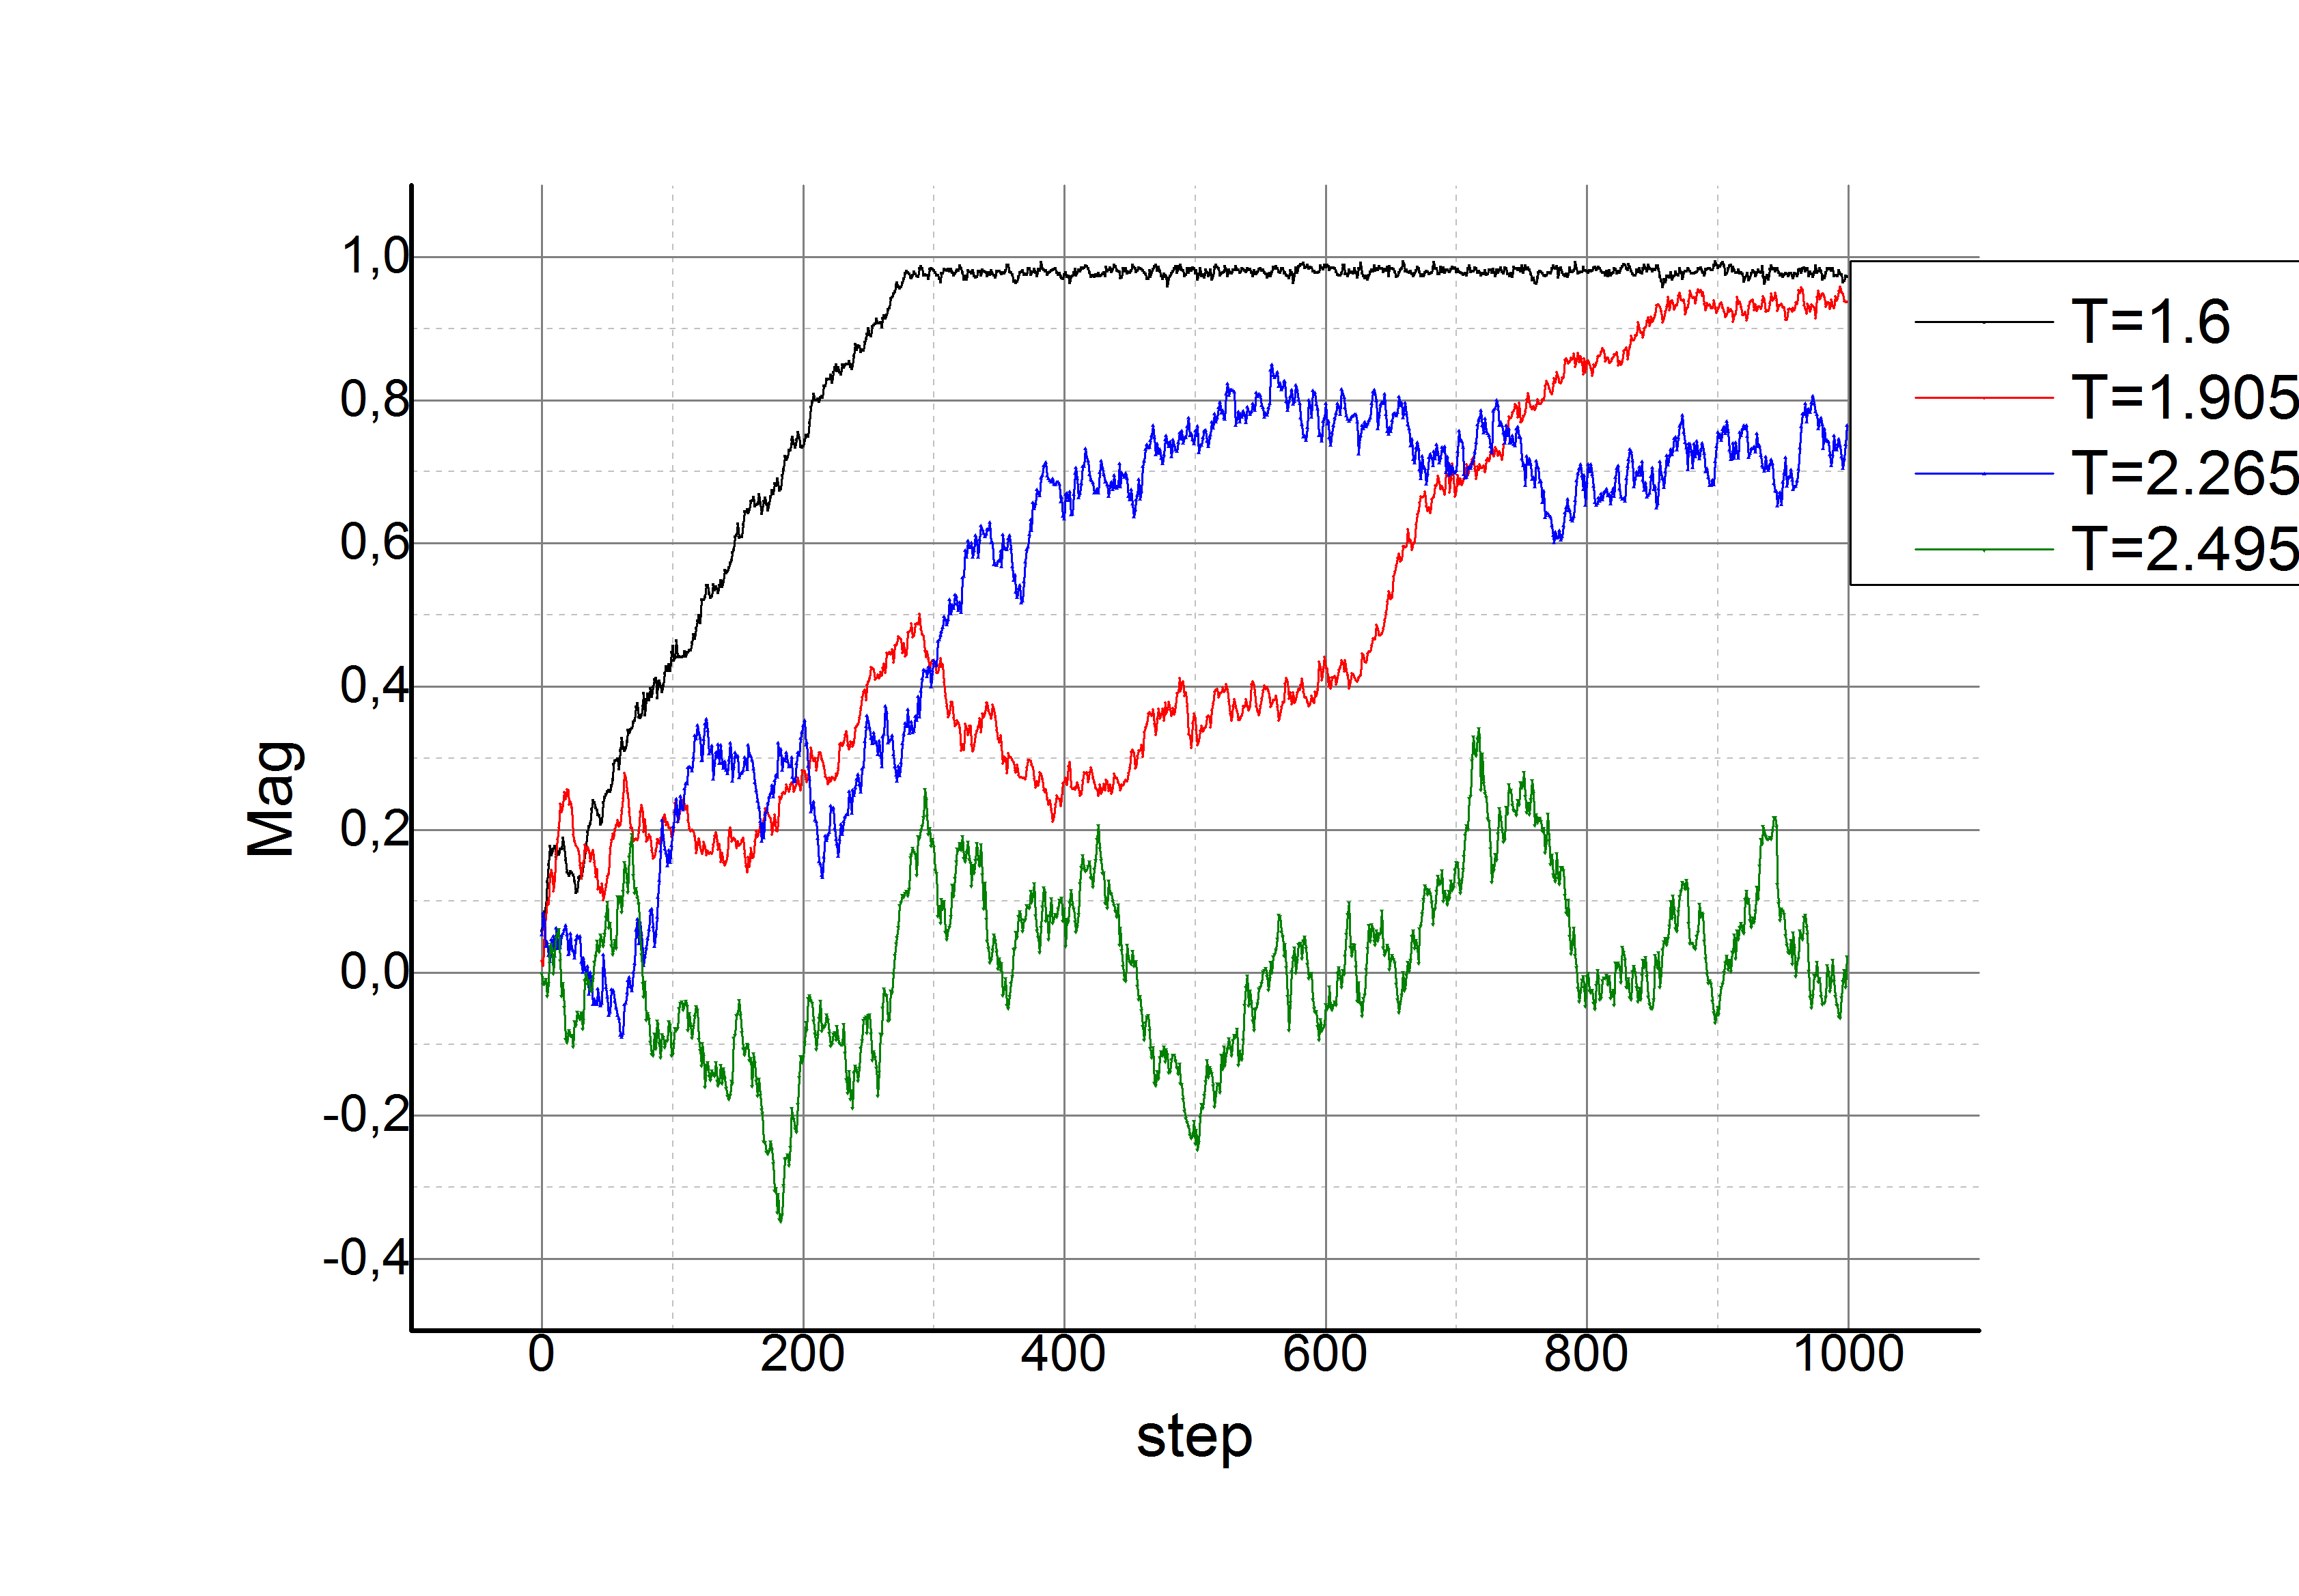
\includegraphics[width=0.47\textwidth]{../Graph_Export/MP2D/m(Steps)_r.jpg}
}	
	\subfigure[2D: positv parallele Startkonfiguration]{
		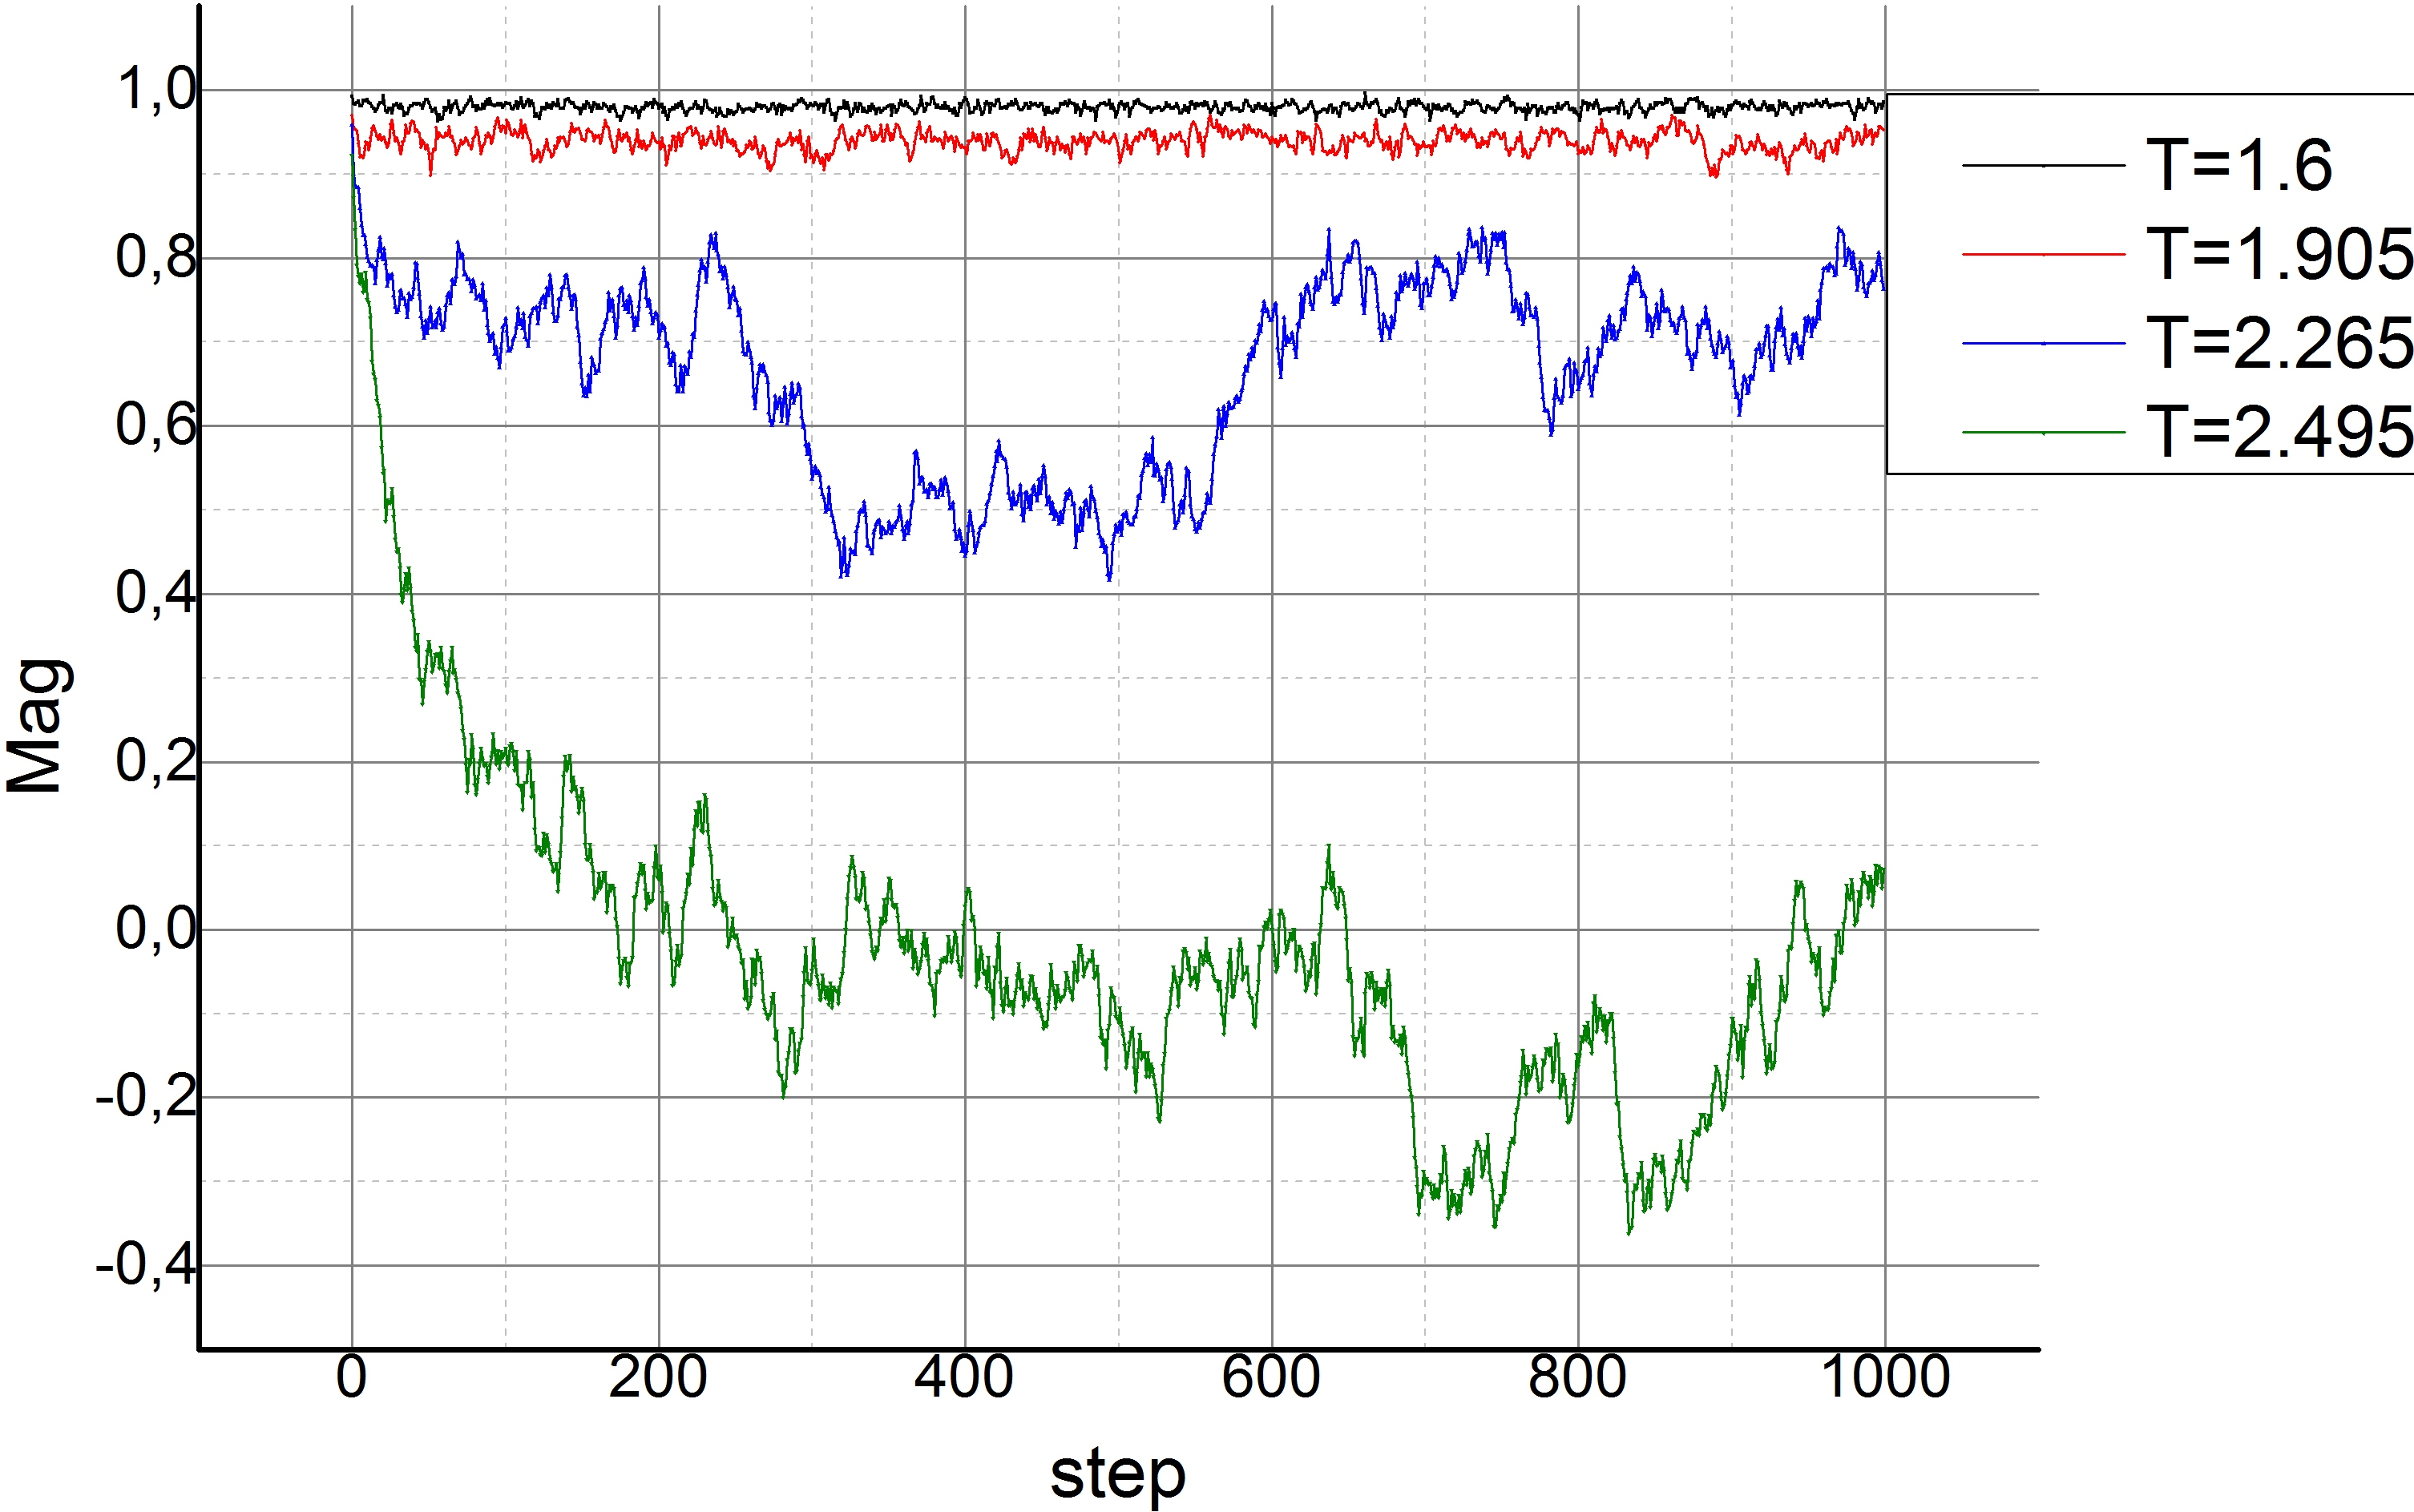
\includegraphics[width=0.47\textwidth]{../Graph_Export/MP2D/m(Steps)_p.jpg}
}		
	\subfigure[3D: zufällige Startkonfiguration]{
		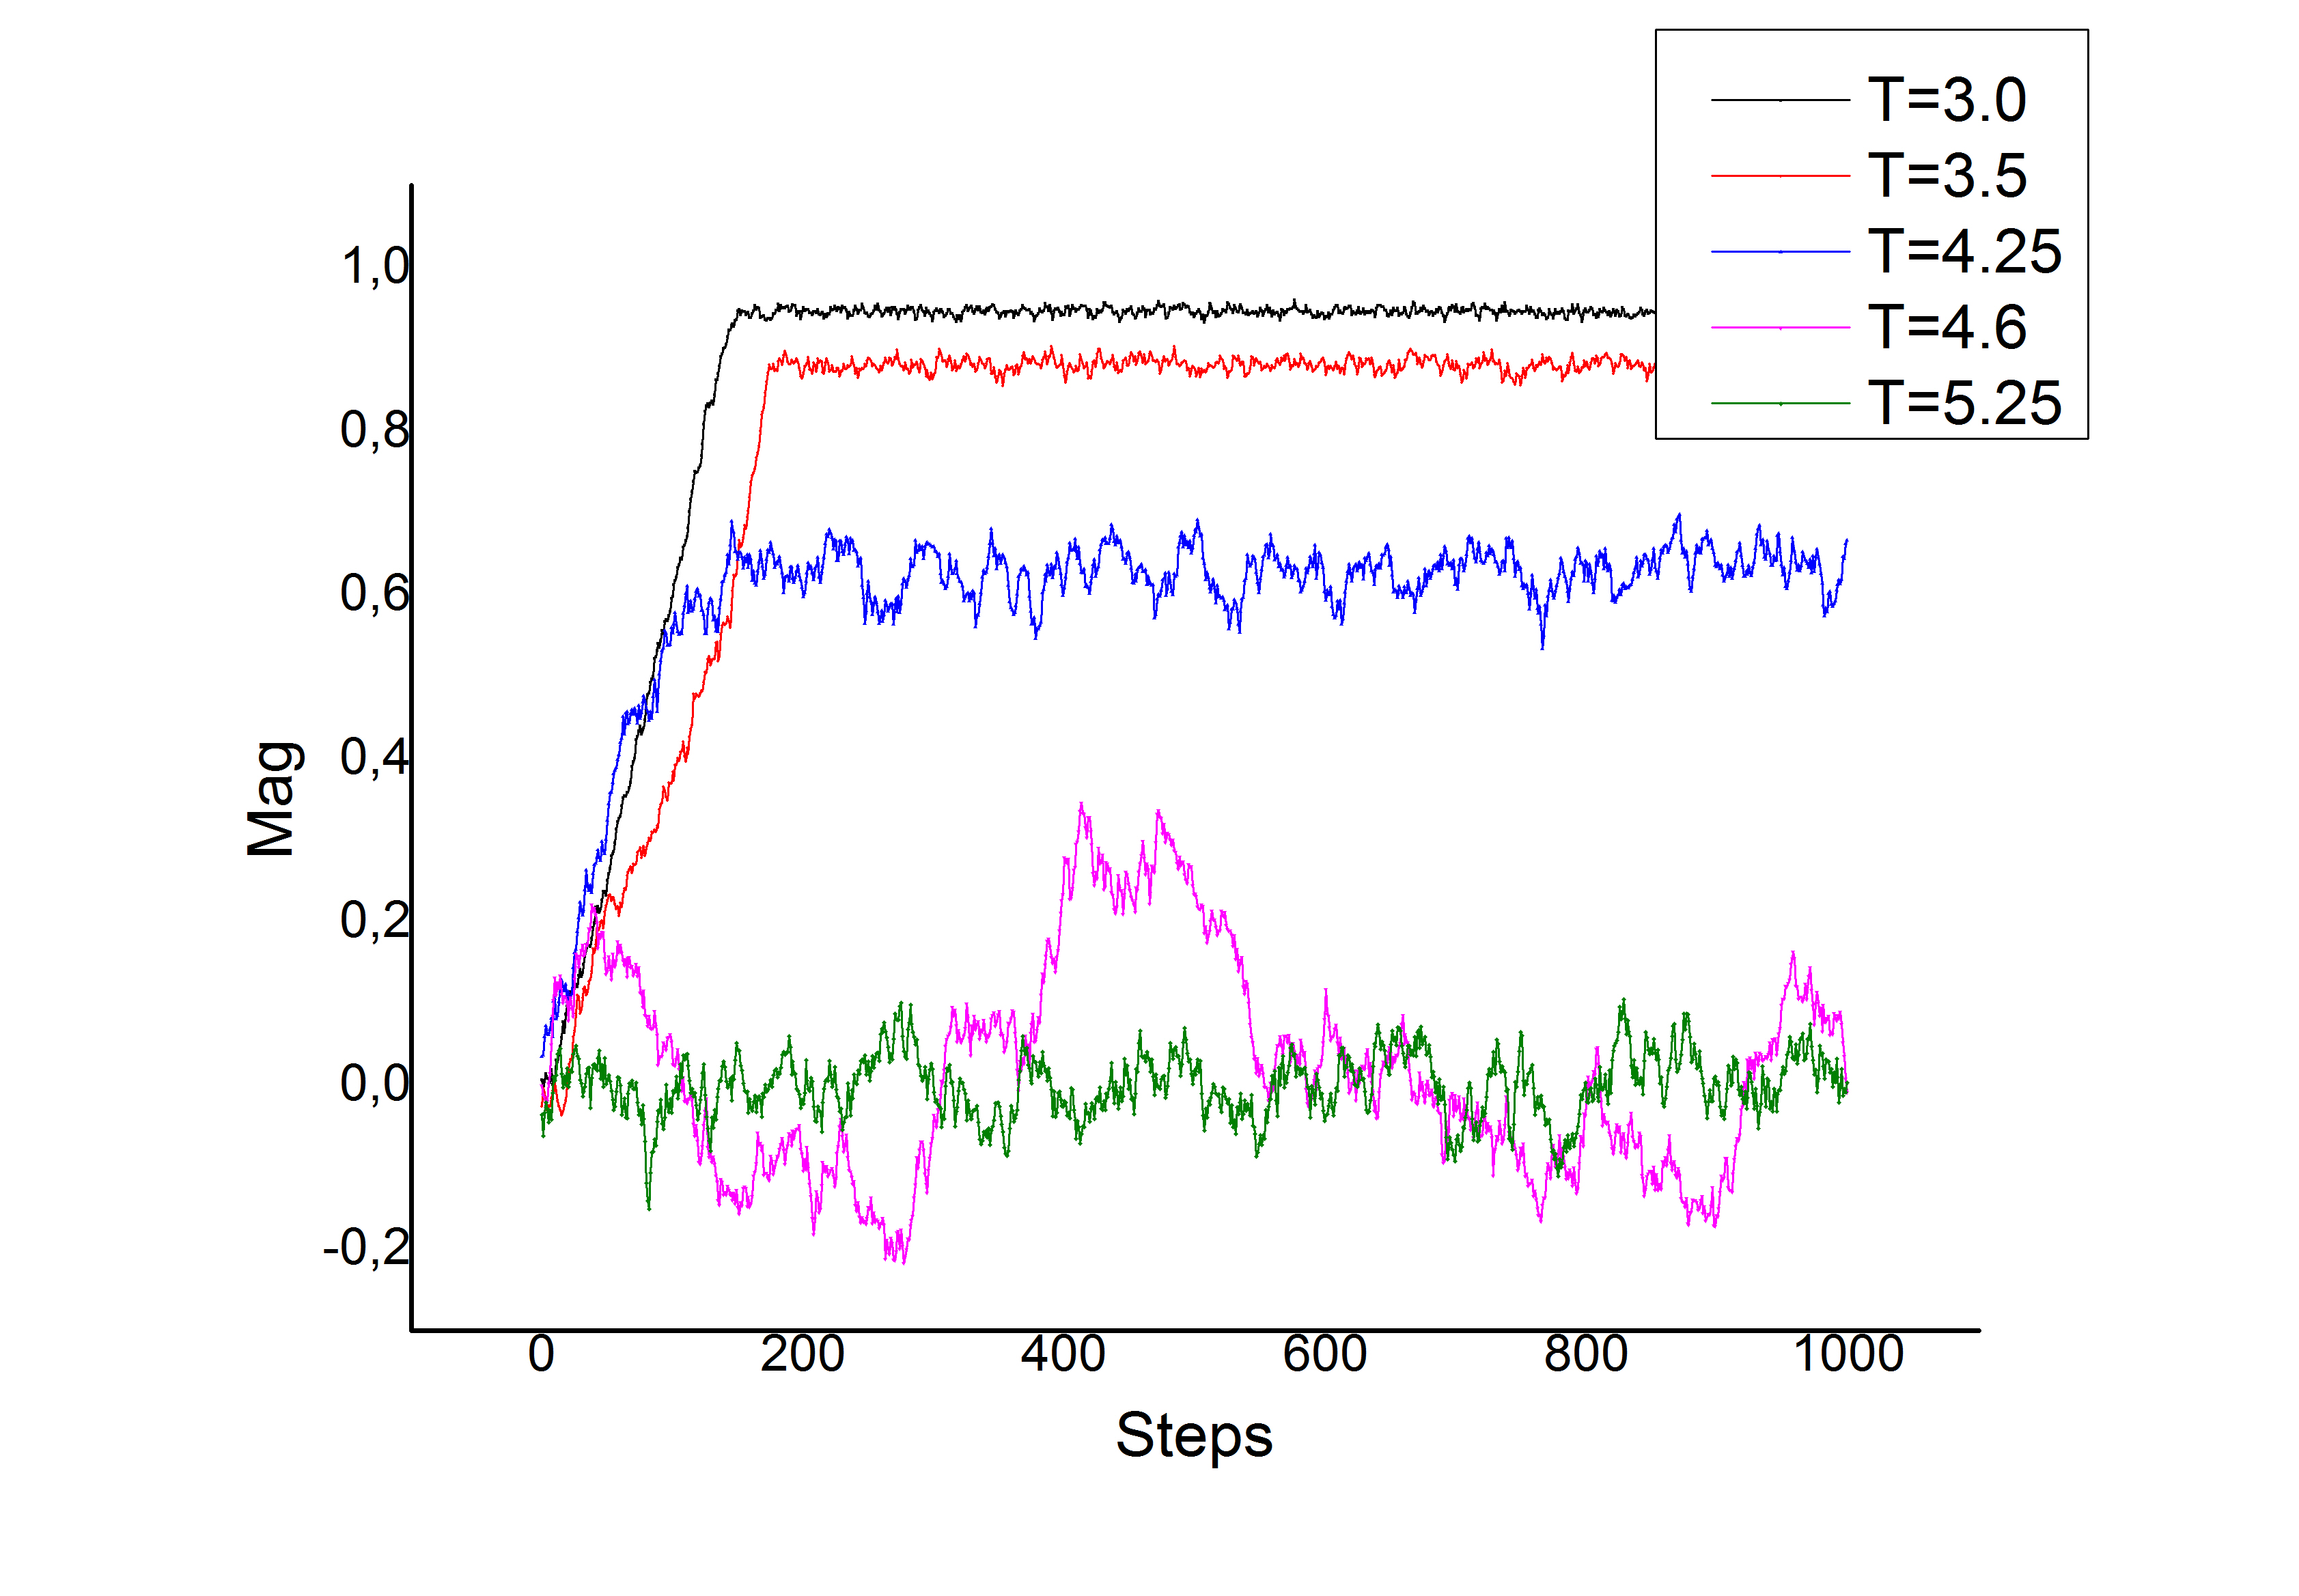
\includegraphics[width=0.47\textwidth]{../Graph_Export/MP3D/m(Steps)_r.jpg}
}	
	\subfigure[3D: positv parallele Startkonfiguration]{
		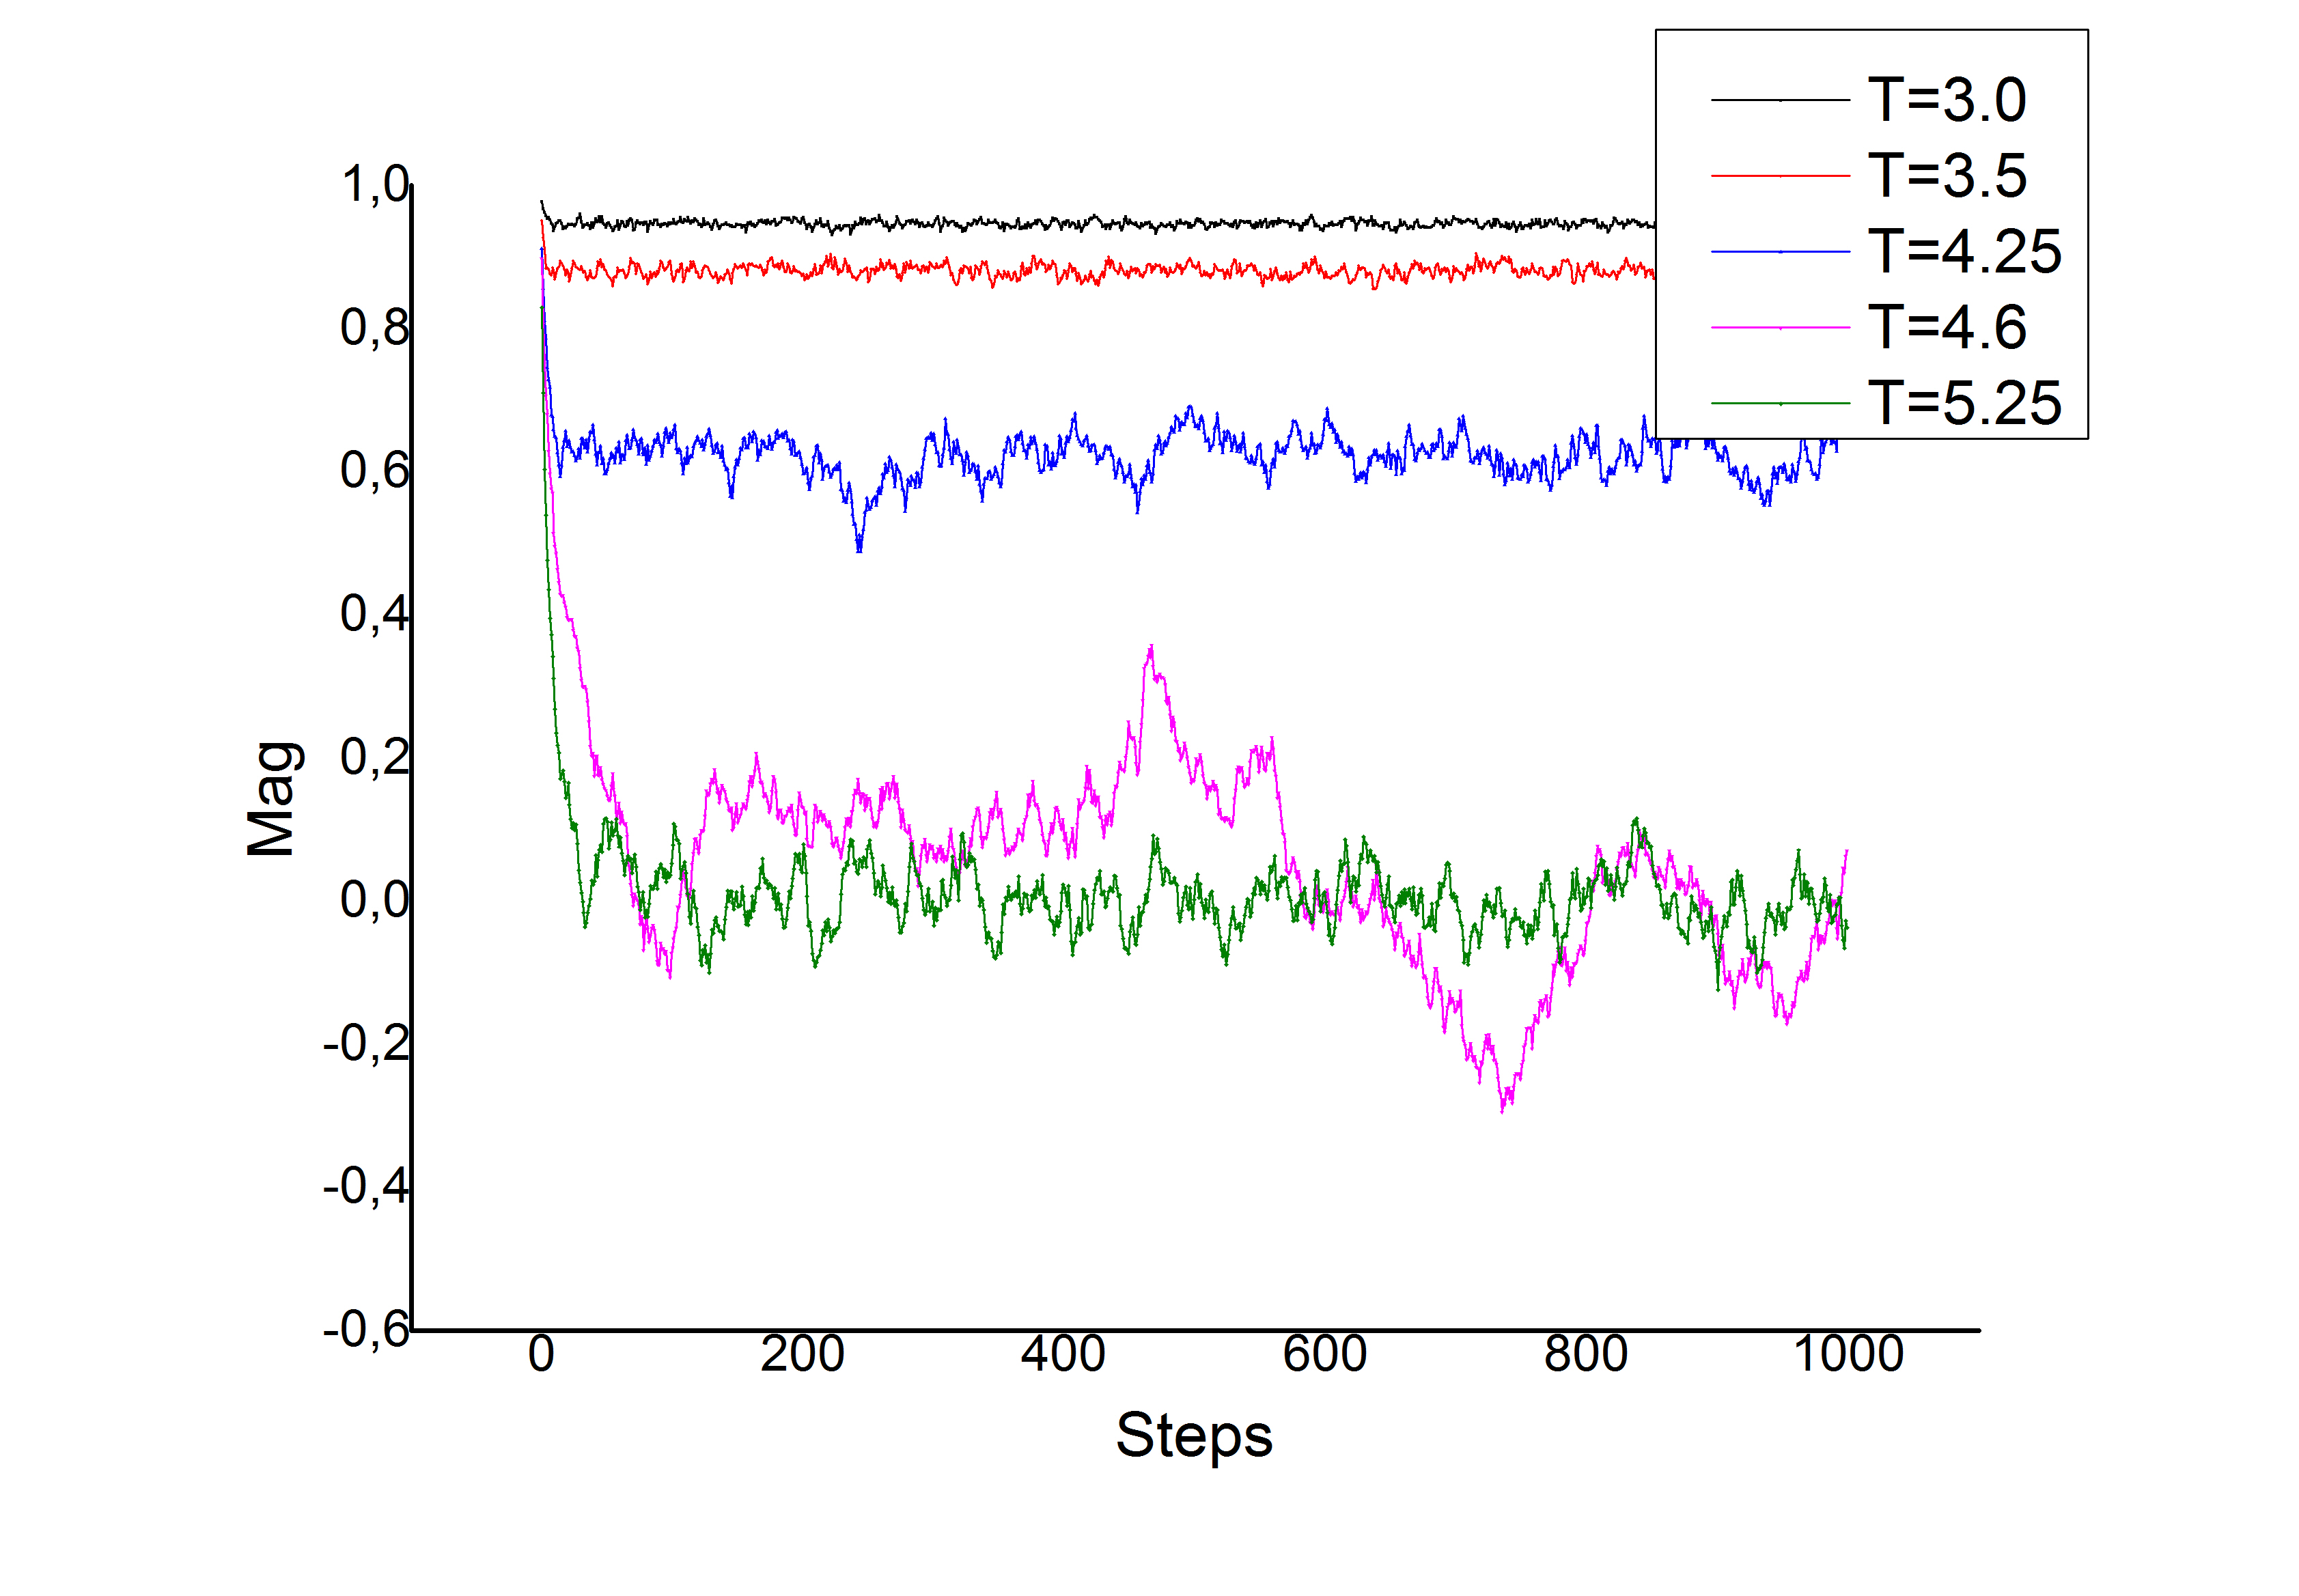
\includegraphics[width=0.47\textwidth]{../Graph_Export/MP3D/m(Steps)_p.jpg}
}		
	\caption{Konvergenzverhalten der Magnetisierung im Metropolisalgorithmus für ein zwei- bzw. dreidimensionales Gitter}
	\label{mpkonv}
\end{figure}
Die Magnetisierung ergibt sich aus der durchschnittlichen Magnetisierung eines Spins im Gitter. Eine komplett parallele Ausrichtung ergibt einen Wert von $m_{0}=\pm1$ (Abb. \ref{mp2dconfig}a), bei Werten von $m_{0} \in(0,1)$ haben sich auf dem Gitter sogenannte Weiß’sche Bezirke oder Domänen gebildet (Abb. \ref{mp2dconfig}b), bis schließlich für $m_{0}\approx0$ sich ein “perfektes” Rauschen einstellt (Abb. \ref{mp2dconfig}c).
\begin{figure}[H]
	\centering
	\subfigure[$T=1,0<<T_{c}$]{
		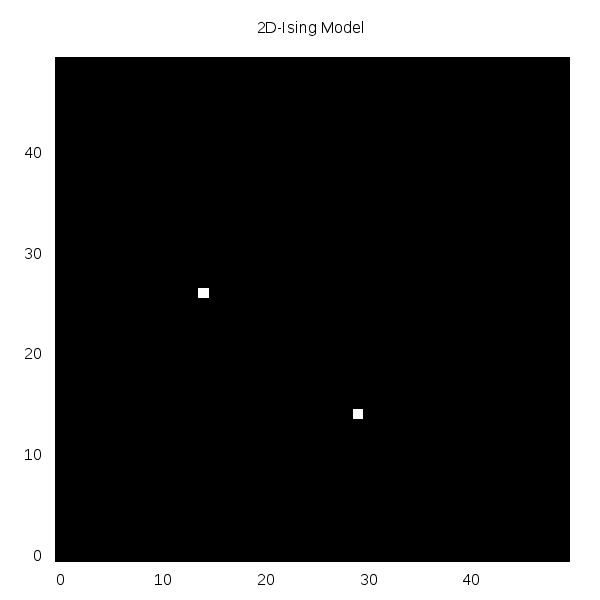
\includegraphics[width=0.25\textwidth]{../Graph_Export/Endbilder/Bild_Ta.png}
}	
	\subfigure[$T=2,24<T_{c}$]{
		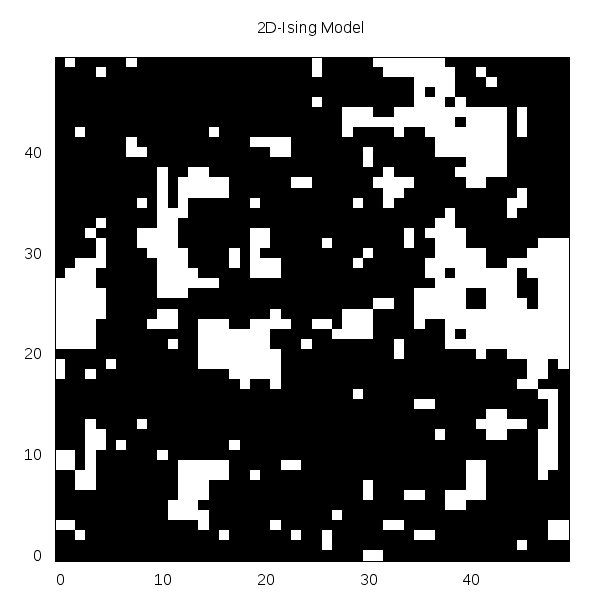
\includegraphics[width=0.25\textwidth]{../Graph_Export/Endbilder/Bild_Tb.png}
}		
	\subfigure[$T=4,0>T_{c}$]{
		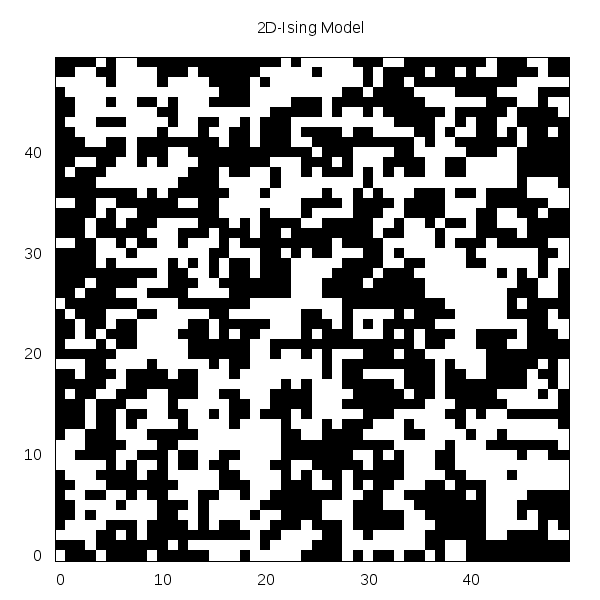
\includegraphics[width=0.25\textwidth]{../Graph_Export/Endbilder/Bild_Tc.png}
}		
	\caption{Abschlusskonfiguration eines 50x50-Gitters in verschiedenen Temperaturbereichen}
	\label{mp2dconfig}
\end{figure}


\subsection{Im Detail: Funktion weiterer Parameter}
\label{met4}

Außer der Wahl der Gittergröße, der Anzahl an Monte-Carlo-Schritten und der Dimension (2D oder 3D) bietet das Programm noch weitere Parameter, mit denen verschiedene Simulationsmodi gestartet werden können.\\
Um nicht nur den Einfluss der Temperatur, sondern auch den des äußeren Magnetfeldes untersuchen zu können, gibt es die Möglichkeit, die zwischen den verschiedenen Simulationen zu variierende Größe zu wählen. So wird entweder der Tempeartur- oder der Magnetfeldbereich zwischen dem als Parameter angegebenen Start- und Endwert mit einer ebenfalls angegebenen Schrittweite durchlaufen.\\
Möchte man das Schaltverhalten des Systems untersuchen, stellt man mit Hilfe eines Parameters ein, dass bei der Variation des Magnetfeldes nicht bei jeder neuen Feldstärke ein zufälliges neues Gitter erstellt wird, sondern auf dem vorhandenen weitergearbeitet wird. Außerdem wird in diesem Fall der angegebene Bereich nicht nur in eine Richtung durchlaufen, sondern anschließend auch zurück, sodass eine Hysterese erkennbar werden kann.\\
Dazu ist es noch möglich, mit einem vollständig ausgerichteten Gitter zu beginnen, sowie die Cluster-Update-Methode zu verwenden oder nicht und zur Veranschaulichung des Systems, einige Zwischenergebnisse als Dateien zu speichern.

\newpage
\section{Ergebnisse und Auswertung}

Durch die Konvergenz der Magnetisierung über eine Monte Carlo Simulation kann nun das Verhalten der Magnetisierung in Abhängigkeit von äußeren Parametern wie Temperatur und Magnetfeld untersucht werden. Hier bei ist zu beachten, dass für die Kopplungskonstante und den Boltzmannfaktor im Folgenden gilt: $J=k_{b}=1$. Insbesondere folgt daraus, dass hier nur Ferromagneten betrachtet werden. Für Antiferromagneten müsste alle Simulationen mit $J=-1$ durchgeführt werden.


\subsection{Phasenübergang zwischen Hoch- und Niedertemperaturphase}
\label{auswT}

Um die Abhängigkeit der Magnetisierung von der Temperatur zu bestimmen, wird jeweils eine Monte Carlo Simulation pro Temperatur für ein konstantes Magnetfeld durch geführt. Dabei kennzeichnet der Temperatur an dem die Magnetisierung auf Null zurückgeht einen kritischen Punkt, an dem ein Phasenübergang stattfindet.


\paragraph{2D-Modell}

\

\

Als erstes wird das 2D-Ising Modell betrachtet. Als Grundlage dient ein 50x50 Gitter. Es wird je Simulation mit einem neuen Gitter gestartet und 1000 Monte Carlo Schritte ausgeführt. 


Zunächst wird die Temperaturabhängigkeit ohne äußeres Feld ($B=0$) untersucht. Durch die analytische Lösung ist die kritische Temperatur ($T_{c}\approx 2,269$), welche den Übergang zwischen Hoch- und Niedertemperaturphase bestimmt, bekannt, sodass ohne weiteres Simulationen von $T=1,5$ bis $T=3,5$ mit einem Schritt von $\Delta T = 0.005$. Hierbei werden zunächst die unterschiedlichen Auswirkungen der Startkonfigurationen betrachtet (Abb. \ref{mp2d0modes}).
\begin{figure}[H]
	\centering
	\subfigure[Start aus Zufallskonfiguration]{
		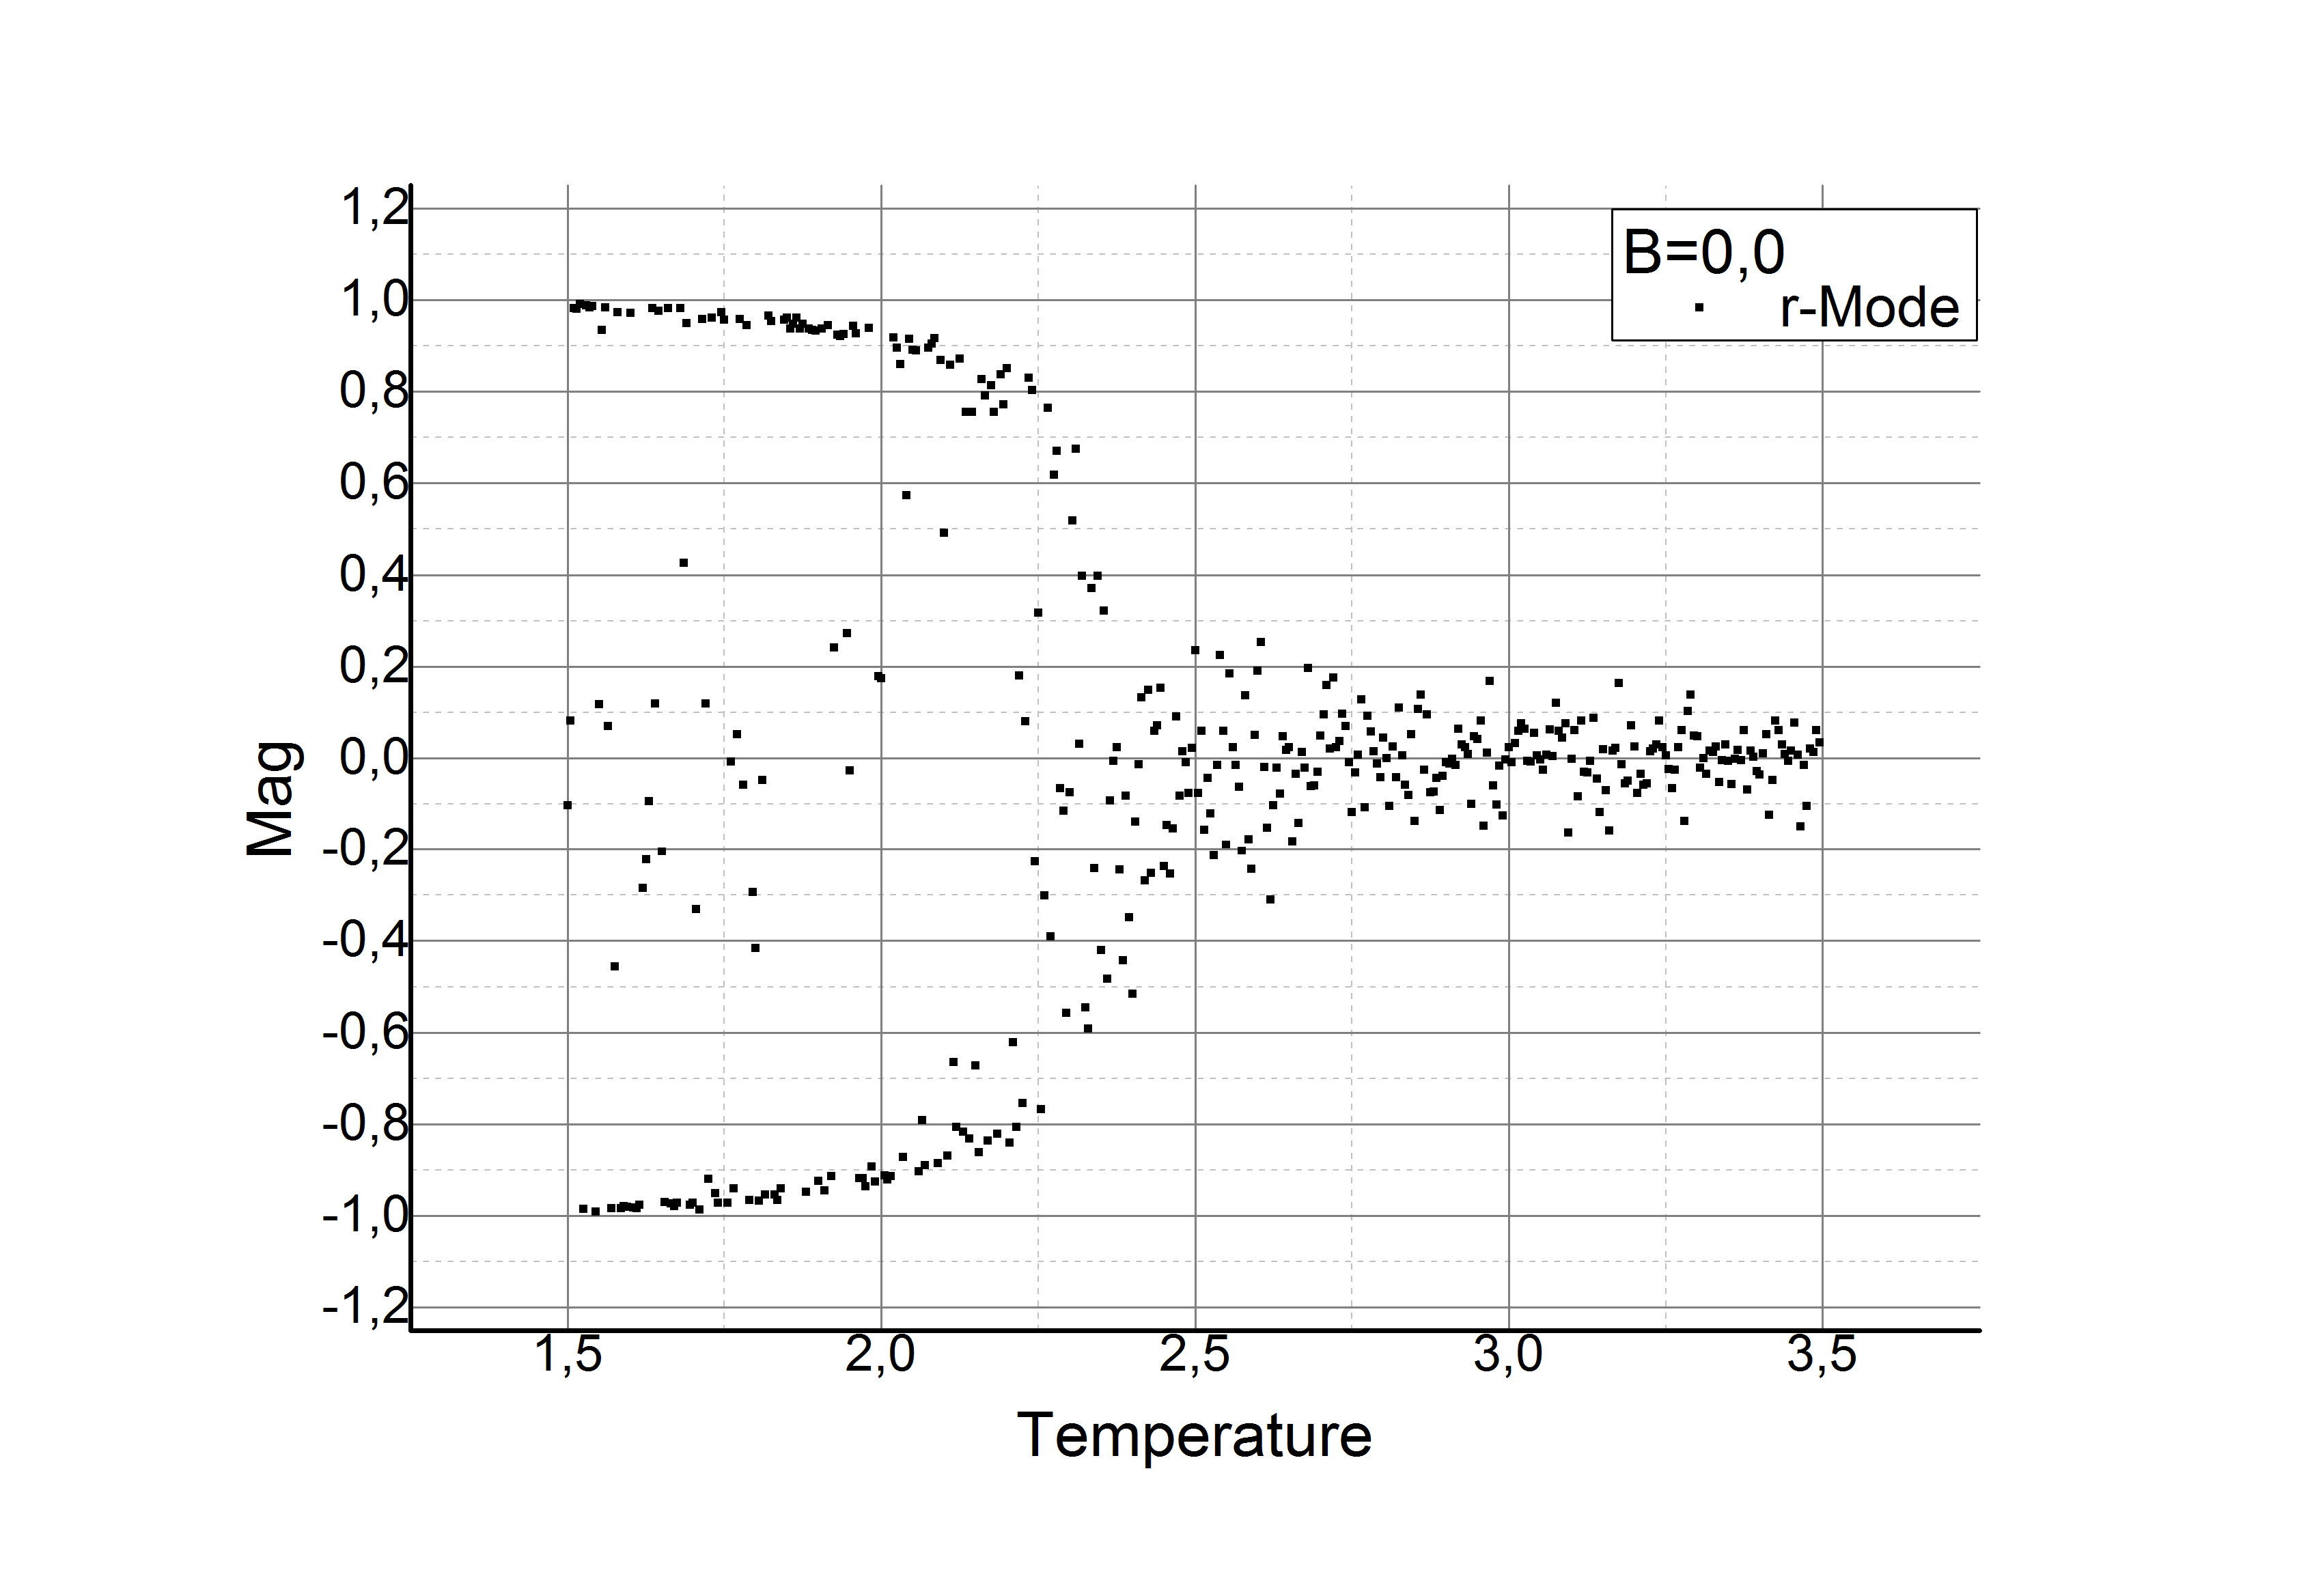
\includegraphics[width=0.47\textwidth]{../Graph_Export/MP2D/m(T)_B=0_rMode_MP2D_50_Plot.jpg}
}	
	\subfigure[Start aus geordneten Konfigurationen]{
		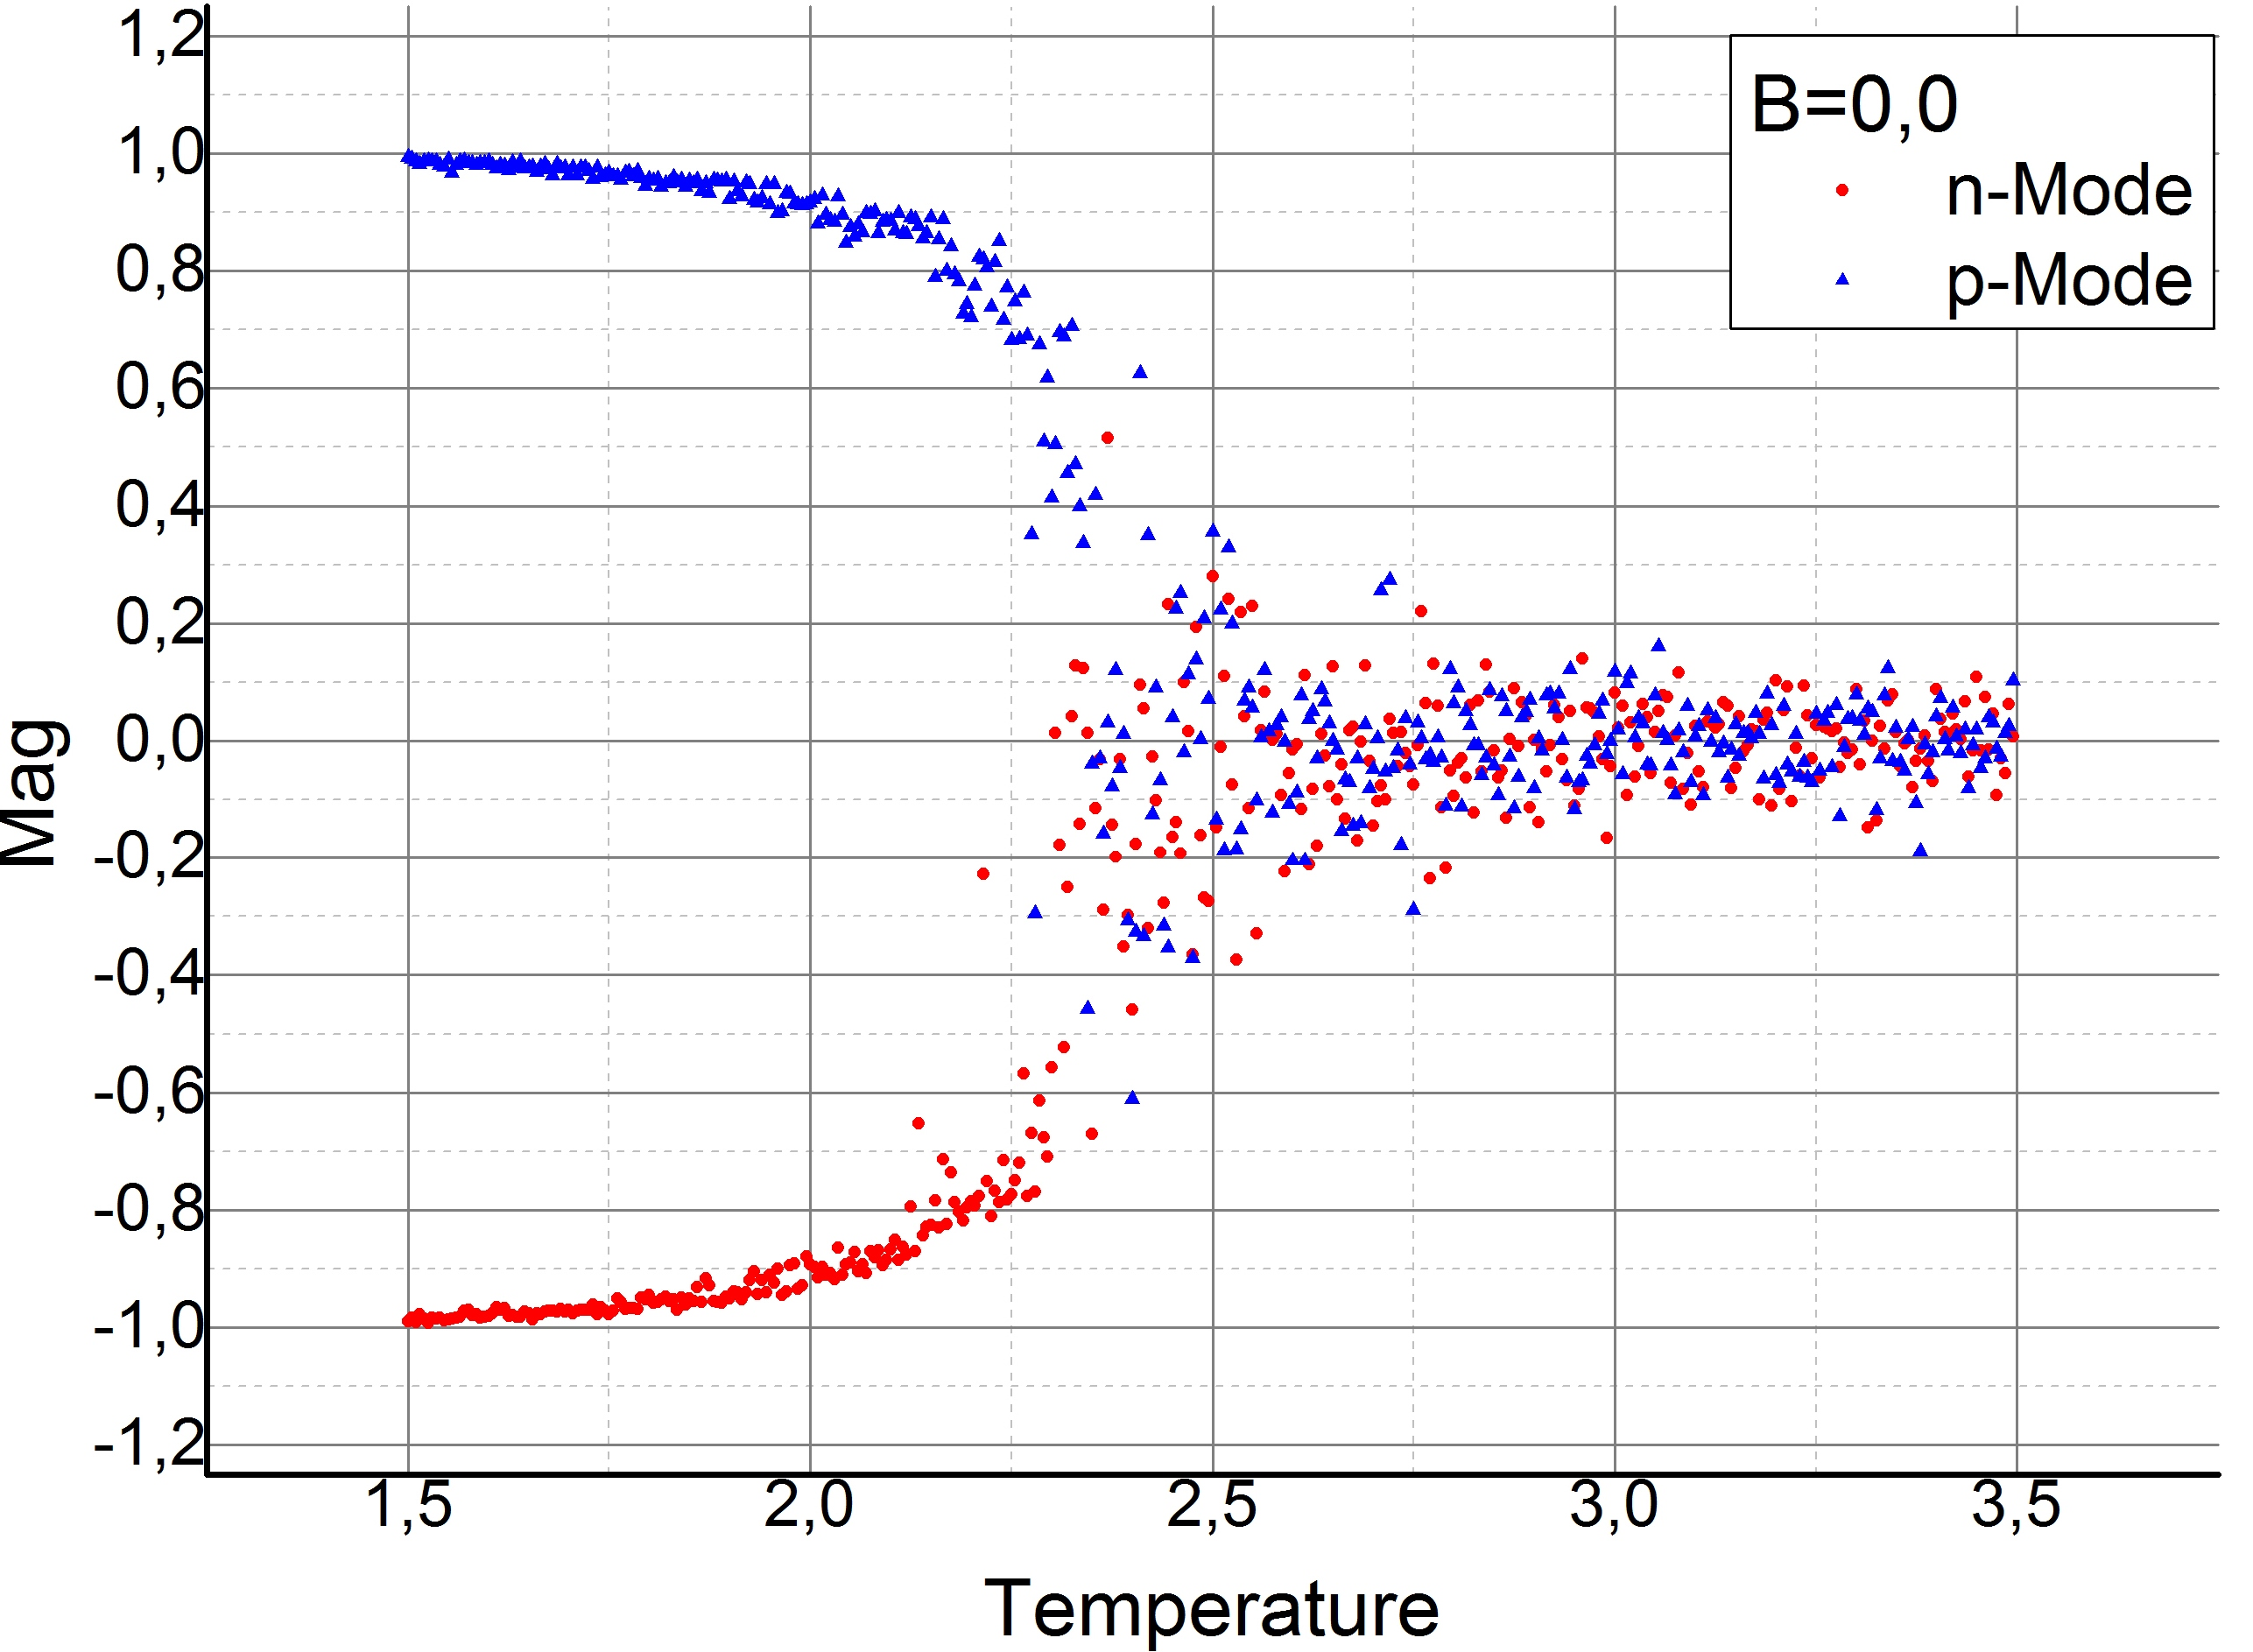
\includegraphics[width=0.47\textwidth]{../Graph_Export/MP2D/m(T)_B=0_pnModes_MP2D_50_Plot.jpg}
}		
	\caption{Temperaturabhängigkeit der Magnetisierung im 2D Ising Modells via Metropolisalgorithmus ohne äußeres Feld}
	\label{mp2d0modes}
\end{figure}
Es ist erkennbar, dass sich die Wahl der Startkonfiguration nicht auf den grundsätzlichen Verlauf der Kurve auswirkt. Dabei sollten allerdings 2 Aspekte beachtet werden. Erstens erkennt man bei Start in einer zufälligen Konfiguration einige Ausreißer im Bereich $T<T_{c}$, in denen einige Simulationen offensichtlich nicht konvergierten. Zweitens führt eine positive Startkonfiguration trivialerweise zu einer Konvergenz zum positiven Wert $m_{0}$ und umgekehrt. Daraus folgt, dass es für diesen Bereich zwei Energieminima bei $\pm m_{0}$ gibt, welche bei Start in zufälliger Konfiguration gleich wahrscheinlich erreicht werden können, bei geordneter Startkonfiguration jedoch nur näheres erreicht wird. Gleich bleibt jedoch das große Rauschen um $T_{c}$, welches zu einer großen Ungenauigkeit bei der Bestimmung der Curie-Temperatur führt, jedoch liegt sie mit einer Abschätzung von $T_{c}\approx 2,26\pm 0,02$ absolut im erwarteten Bereich. Hier ist eine Unstetigkeit in der ersten Ableitung zu erkennen, welche den Phasenübergang kennzeichnet. Auch ein kleineres Rauschen für $T>T_{c}$ mit einer Bandbreite von $\pm 0,2 = 0,4$ ist in allen Simulationen vorhanden. Um dieses Rauschen zu minimieren könnte man mit größeren Gittern arbeiten, diese erzeugen jedoch auch mehr Ausreißer im Bereich $T<T_{c}$.


Für eine optimale Auflösung empfiehlt sich für Metropolis Algorithmen ohne äußeres Feld folglich zwei Simulationen, je eine aus positiver und negativer Startkonfiguration.


Nun soll die Auswirkung eines äußeren Feldes auf die Temperaturabhängigkeit betrachtet werden. Dazu wird obige Simulation für die Felder $B=\pm 0,1$ im Bereich $T=1,5$ bis $T=5,0$ und $B=\pm 0,4$ im Bereich $T=1,5$ bis $T=7,0$ durchgeführt. Dabei wird die Schrittweite auf $\Delta T = 0.01$ bzw. $\Delta T = 0.02$ erhöht (Abb. \ref{mp2db}). Für Simulationen mit äußerem Feld kann bedenkenlos aus zufälliger Konfiguration gestartet werden, da das angelegte Feld Außreißer für $T<T_{c}$ verhiindert und das Vorzeichen des angenommen Werts bestimmt. Bei geordneter Startkonfiguration ist die zweite Bedingung nicht zwingend erfüllt, wie Kapitel \ref{auswB} zeigen wird.
\begin{figure}[H]
	\centering
	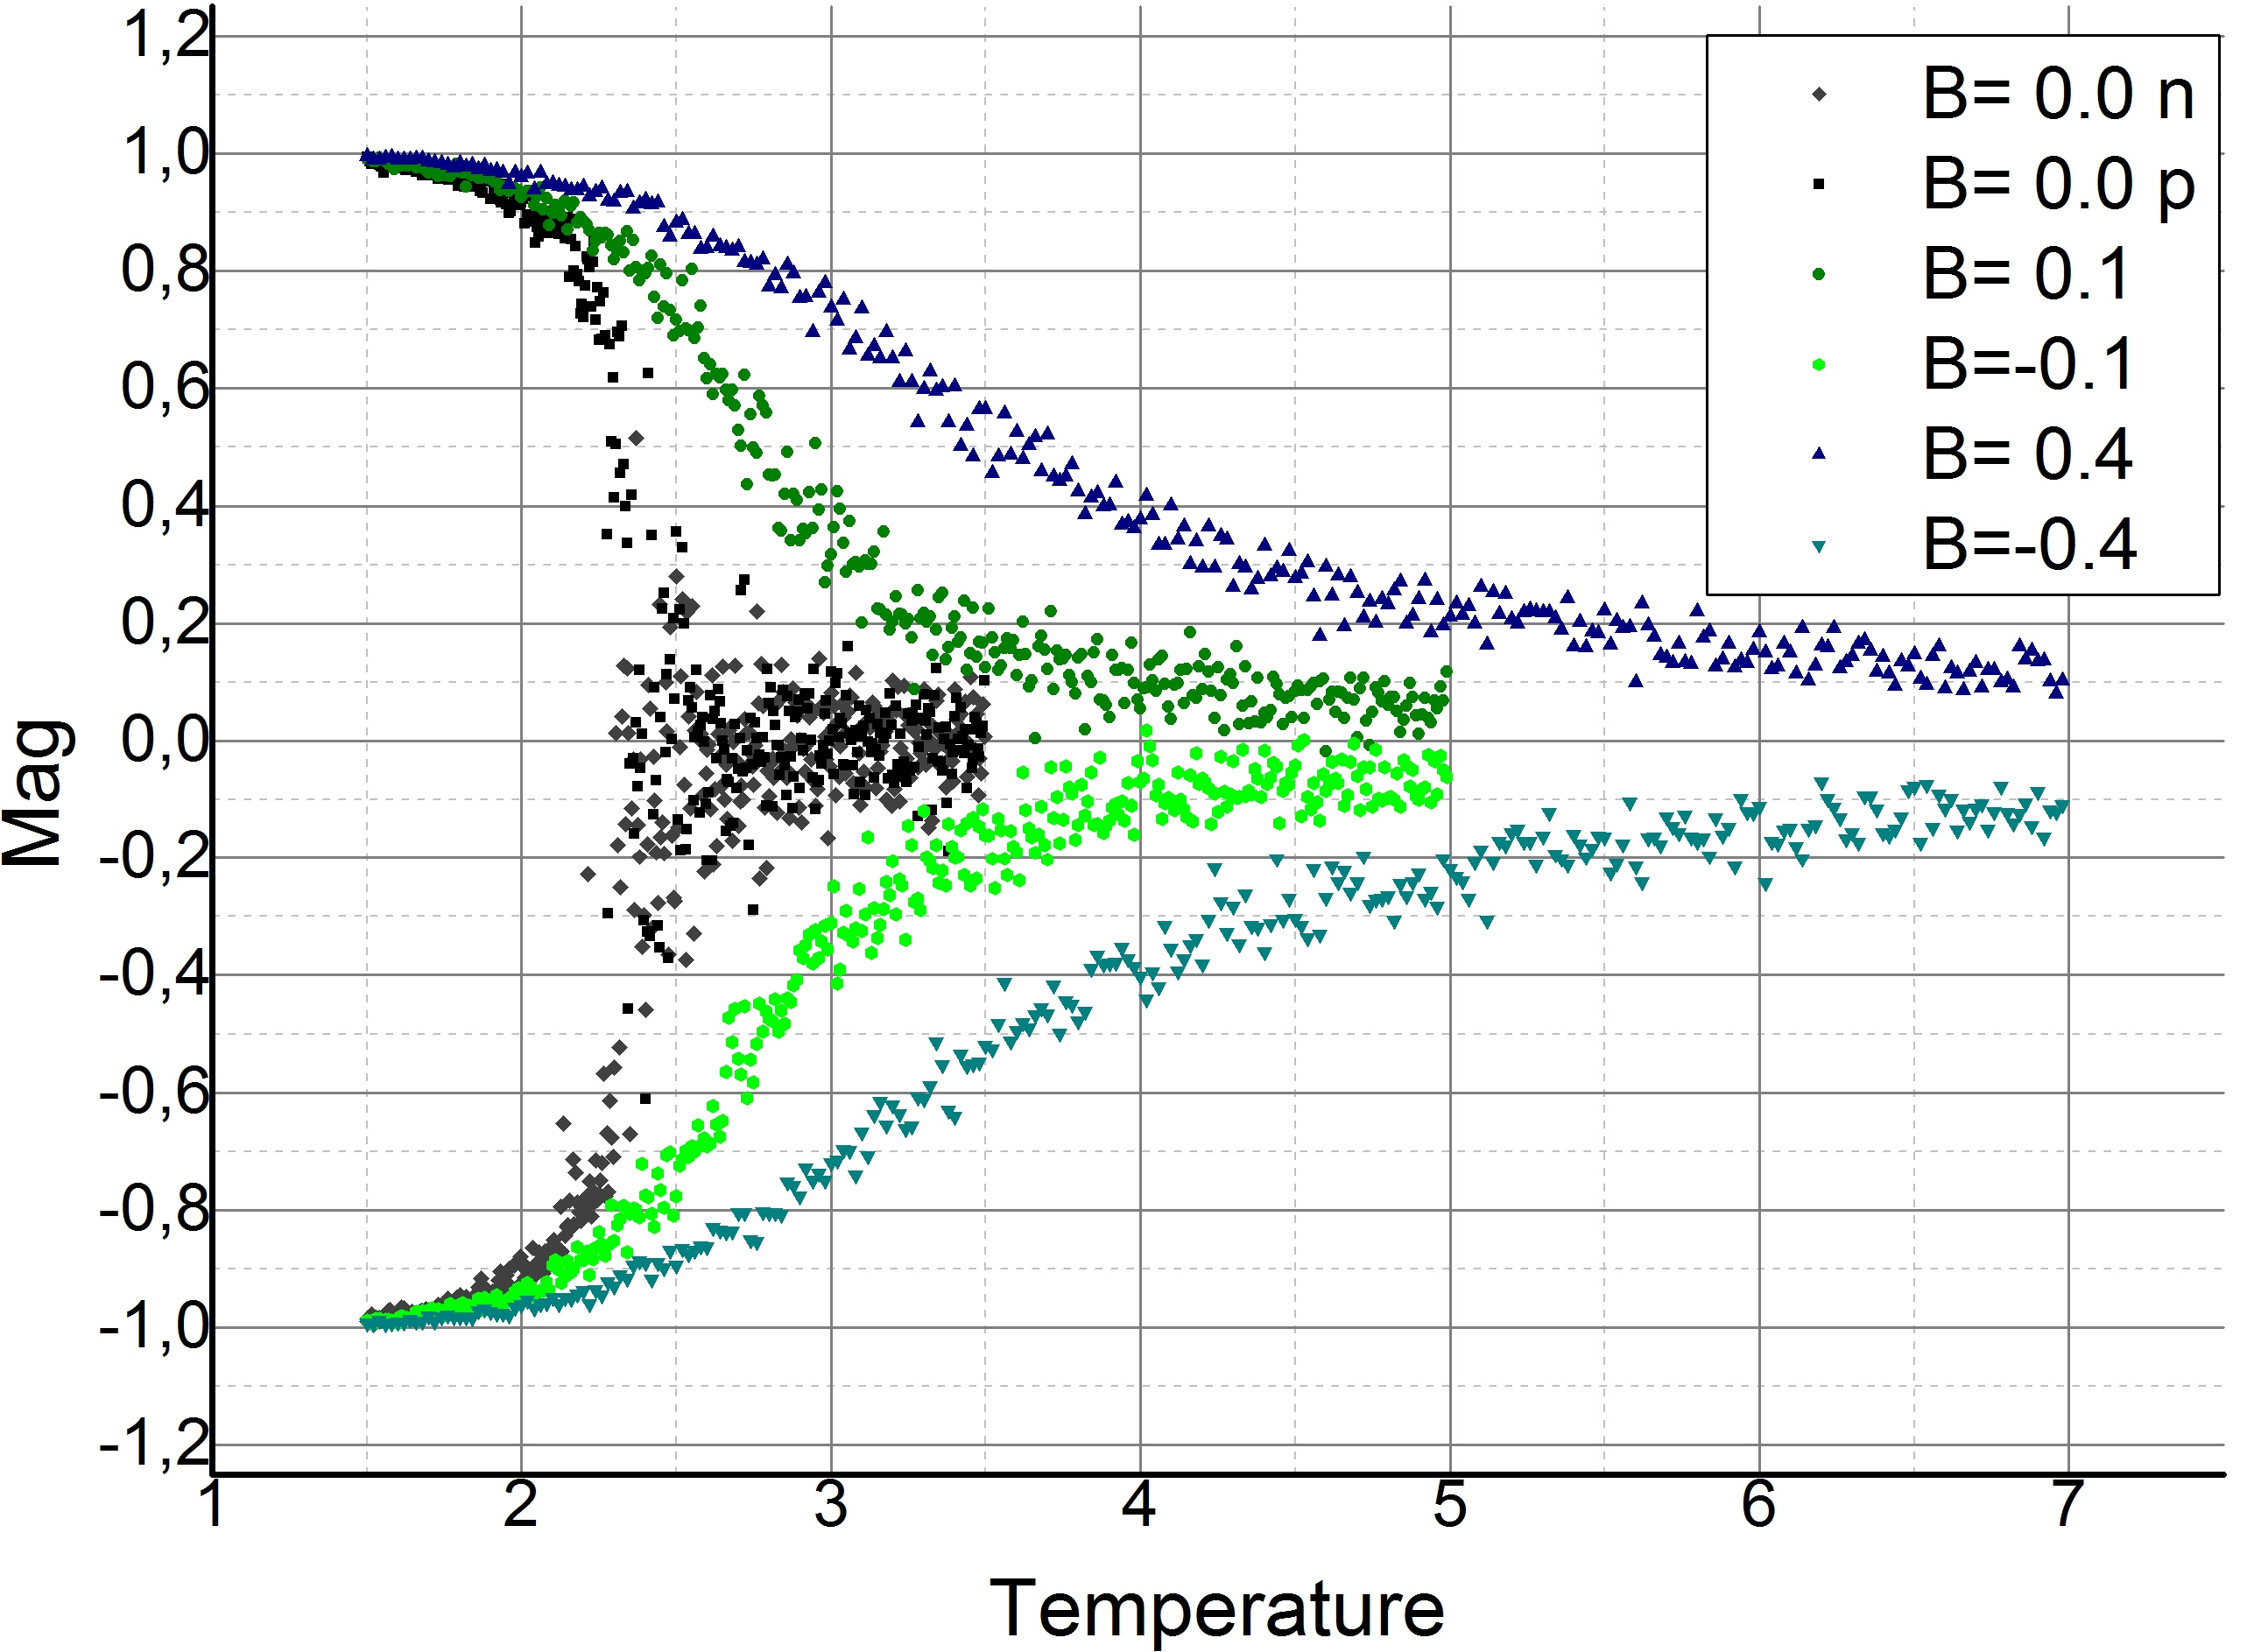
\includegraphics[width=0.8\textwidth]{../Graph_Export/MP2D/m(T)_MP2D_50_Plot.jpg}	
	\caption{Temperaturabhängigkeit der Magnetisierung im 2D Ising Modells via Metropolisalgorithmus für verschiedene äußere Felder}
	\label{mp2db}
\end{figure}
Während ohne äußeres Feld die Magnetisierung an $T_{c}$ steil abfällt und (bis auf ein Rauschen) auf Null zurückgeht, treten bei angelegtem Feld Ausschmierungen auf, sodass sich die Kurve asymptotisch der Null nähert und man weiterhin zwischen negativem und positivem Arm unterscheiden kann, welche dan jeweils mit etwa $0,2$ zum Grundrauschen beitragen. Auch nimmt die Größe der Ausschmierung bei stärkeren Feldern weiter zu.


\paragraph{3DModell}

\

\

Nun wird die Temperatur im 3D-IsingModell untersucht. Um in vertretbarem Rechenaufwand zu bleiben, wird ein 20x20x20 Gitter benutzt. Jede Simulation startet mit einem neuem Gitter und führt wiederum 1000 Schritte aus.


Als erstes wird wieder die Auswirkung der Startkonfiguration auf Simulationen ohne äußeres Feld untersucht (Abb. \ref{mp3d0modes}). Die Simulationen laufen jeweils von $T=2,5$ bis $T=6,0$ mit einer Schrittweite von $\Delta T= 0,01$.
\begin{figure}[H]
	\centering
	\subfigure[Start aus Zufallskonfiguration]{
		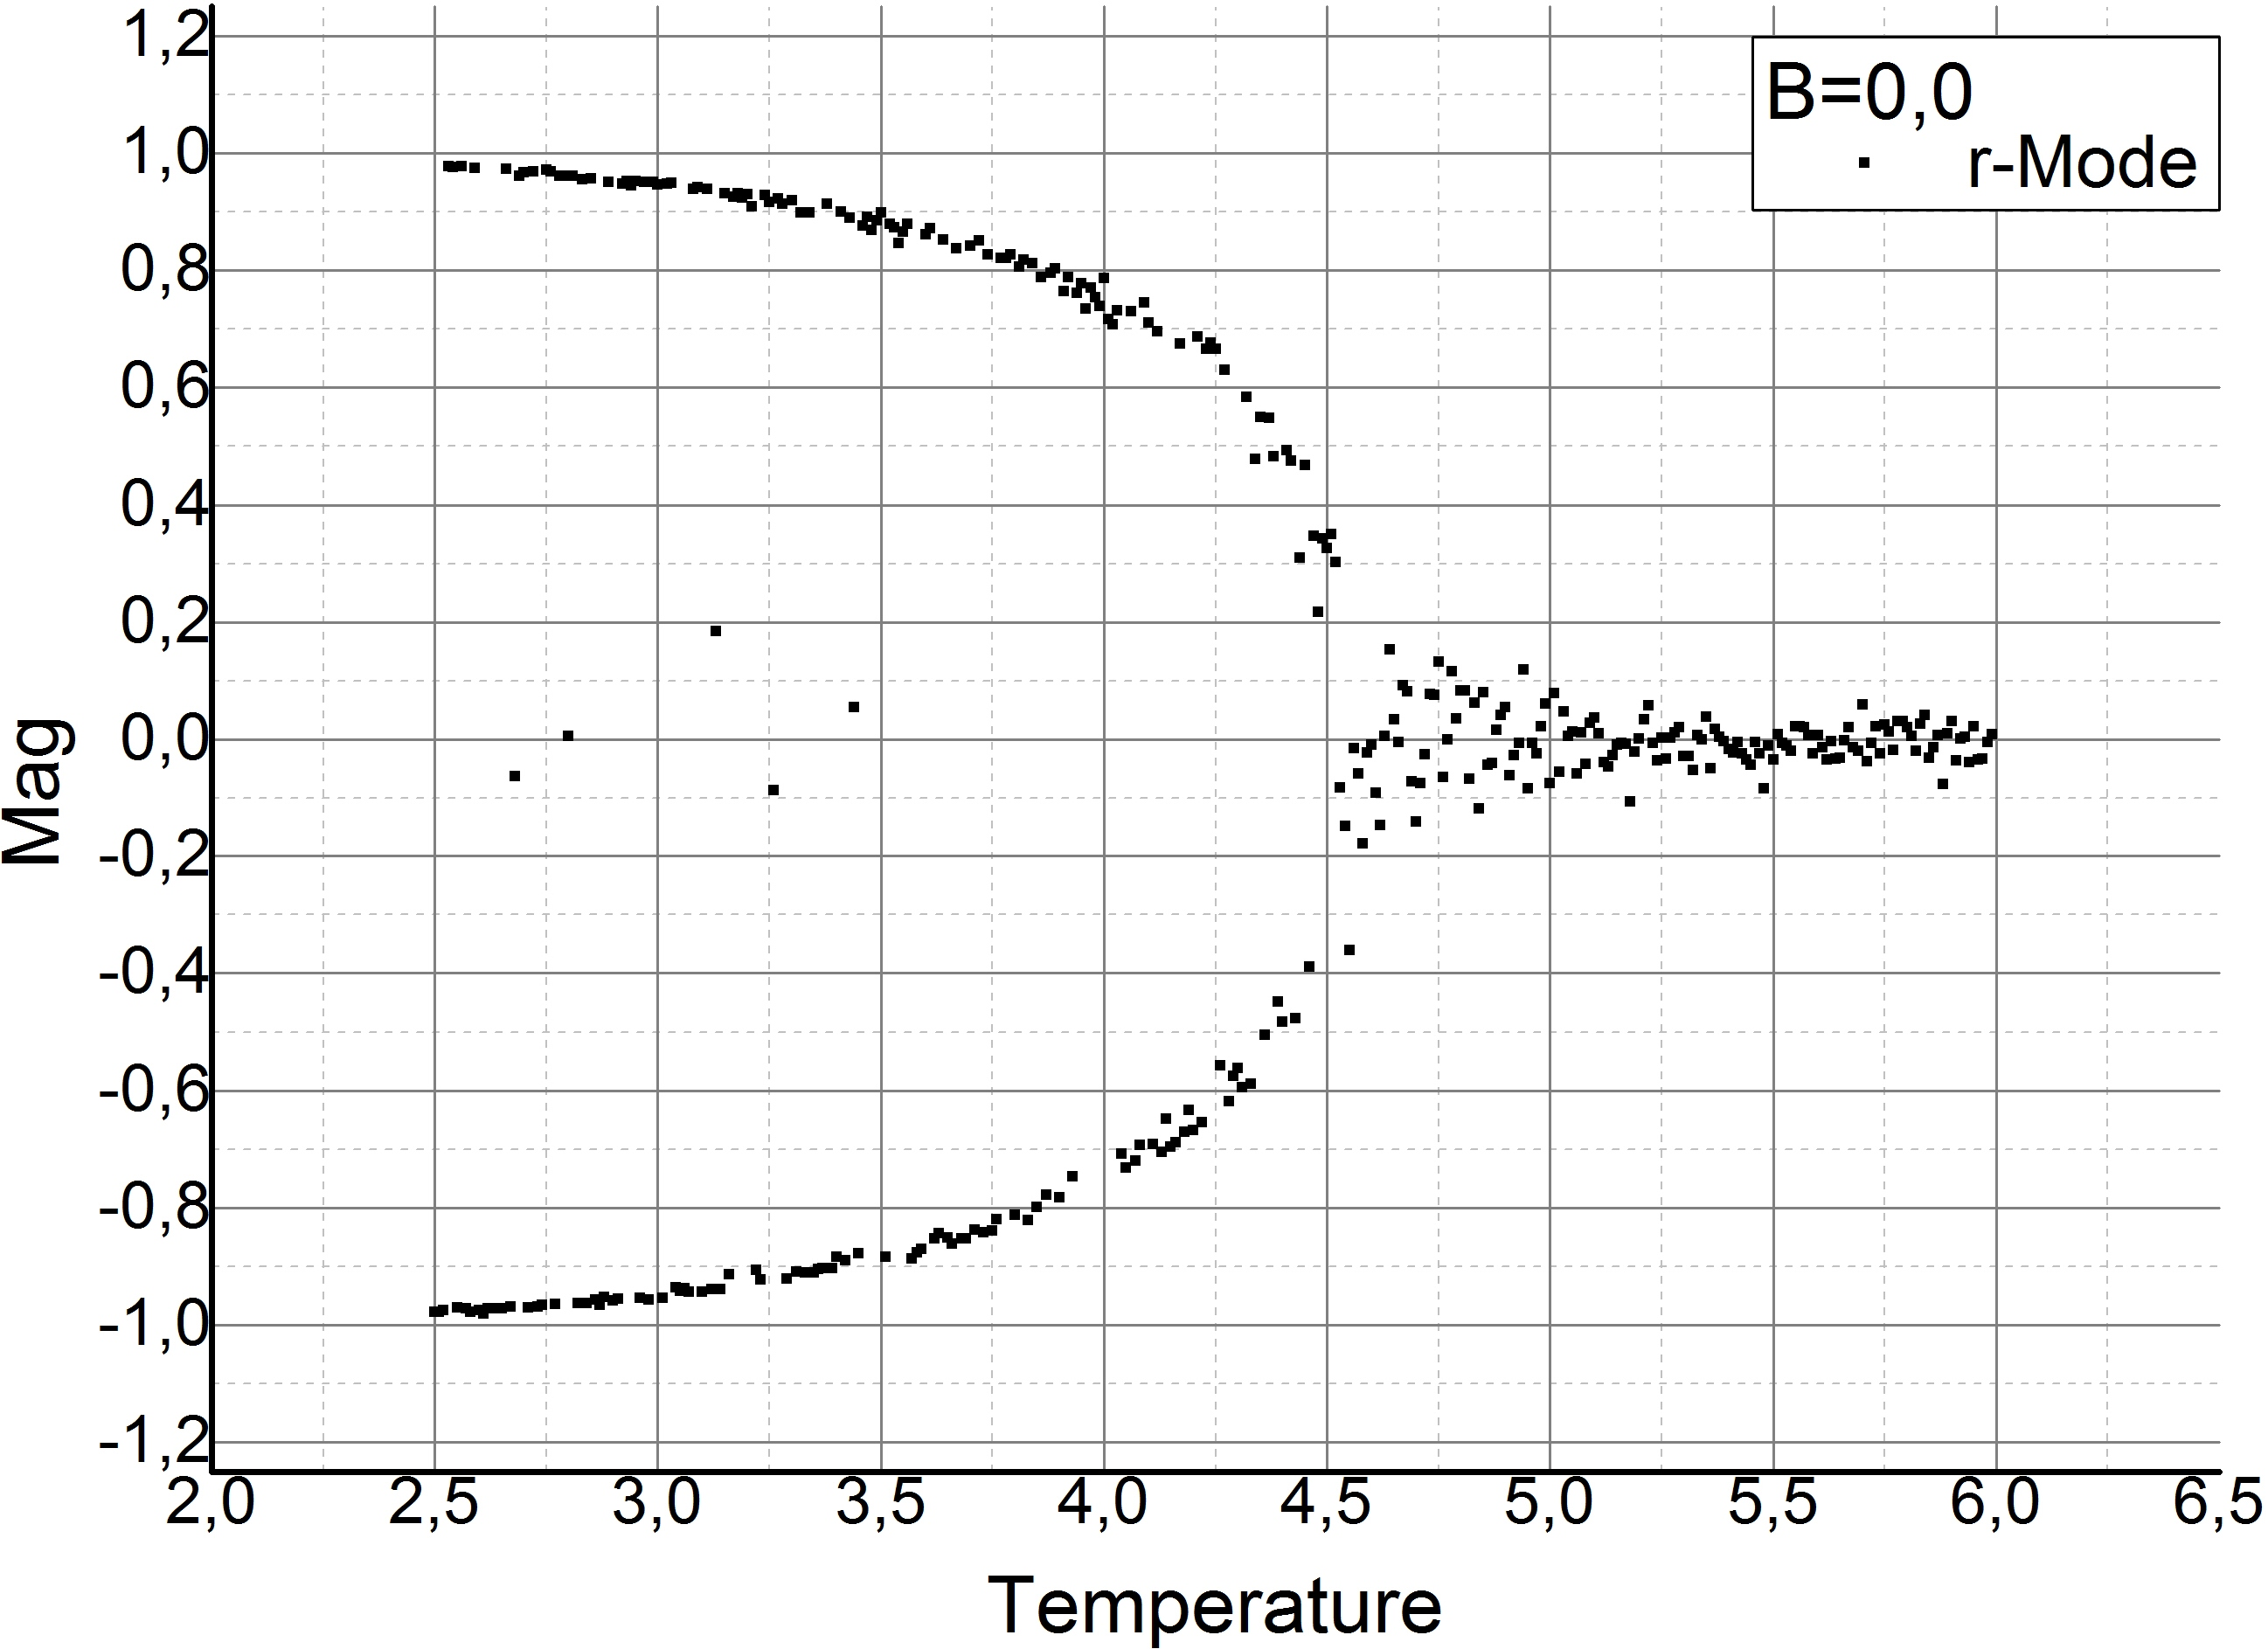
\includegraphics[width=0.47\textwidth]{../Graph_Export/MP3D/m(T)_B=0_rMode_MP3D_Plot.jpg}
}	
	\subfigure[Start aus geordneten Konfigurationen]{
		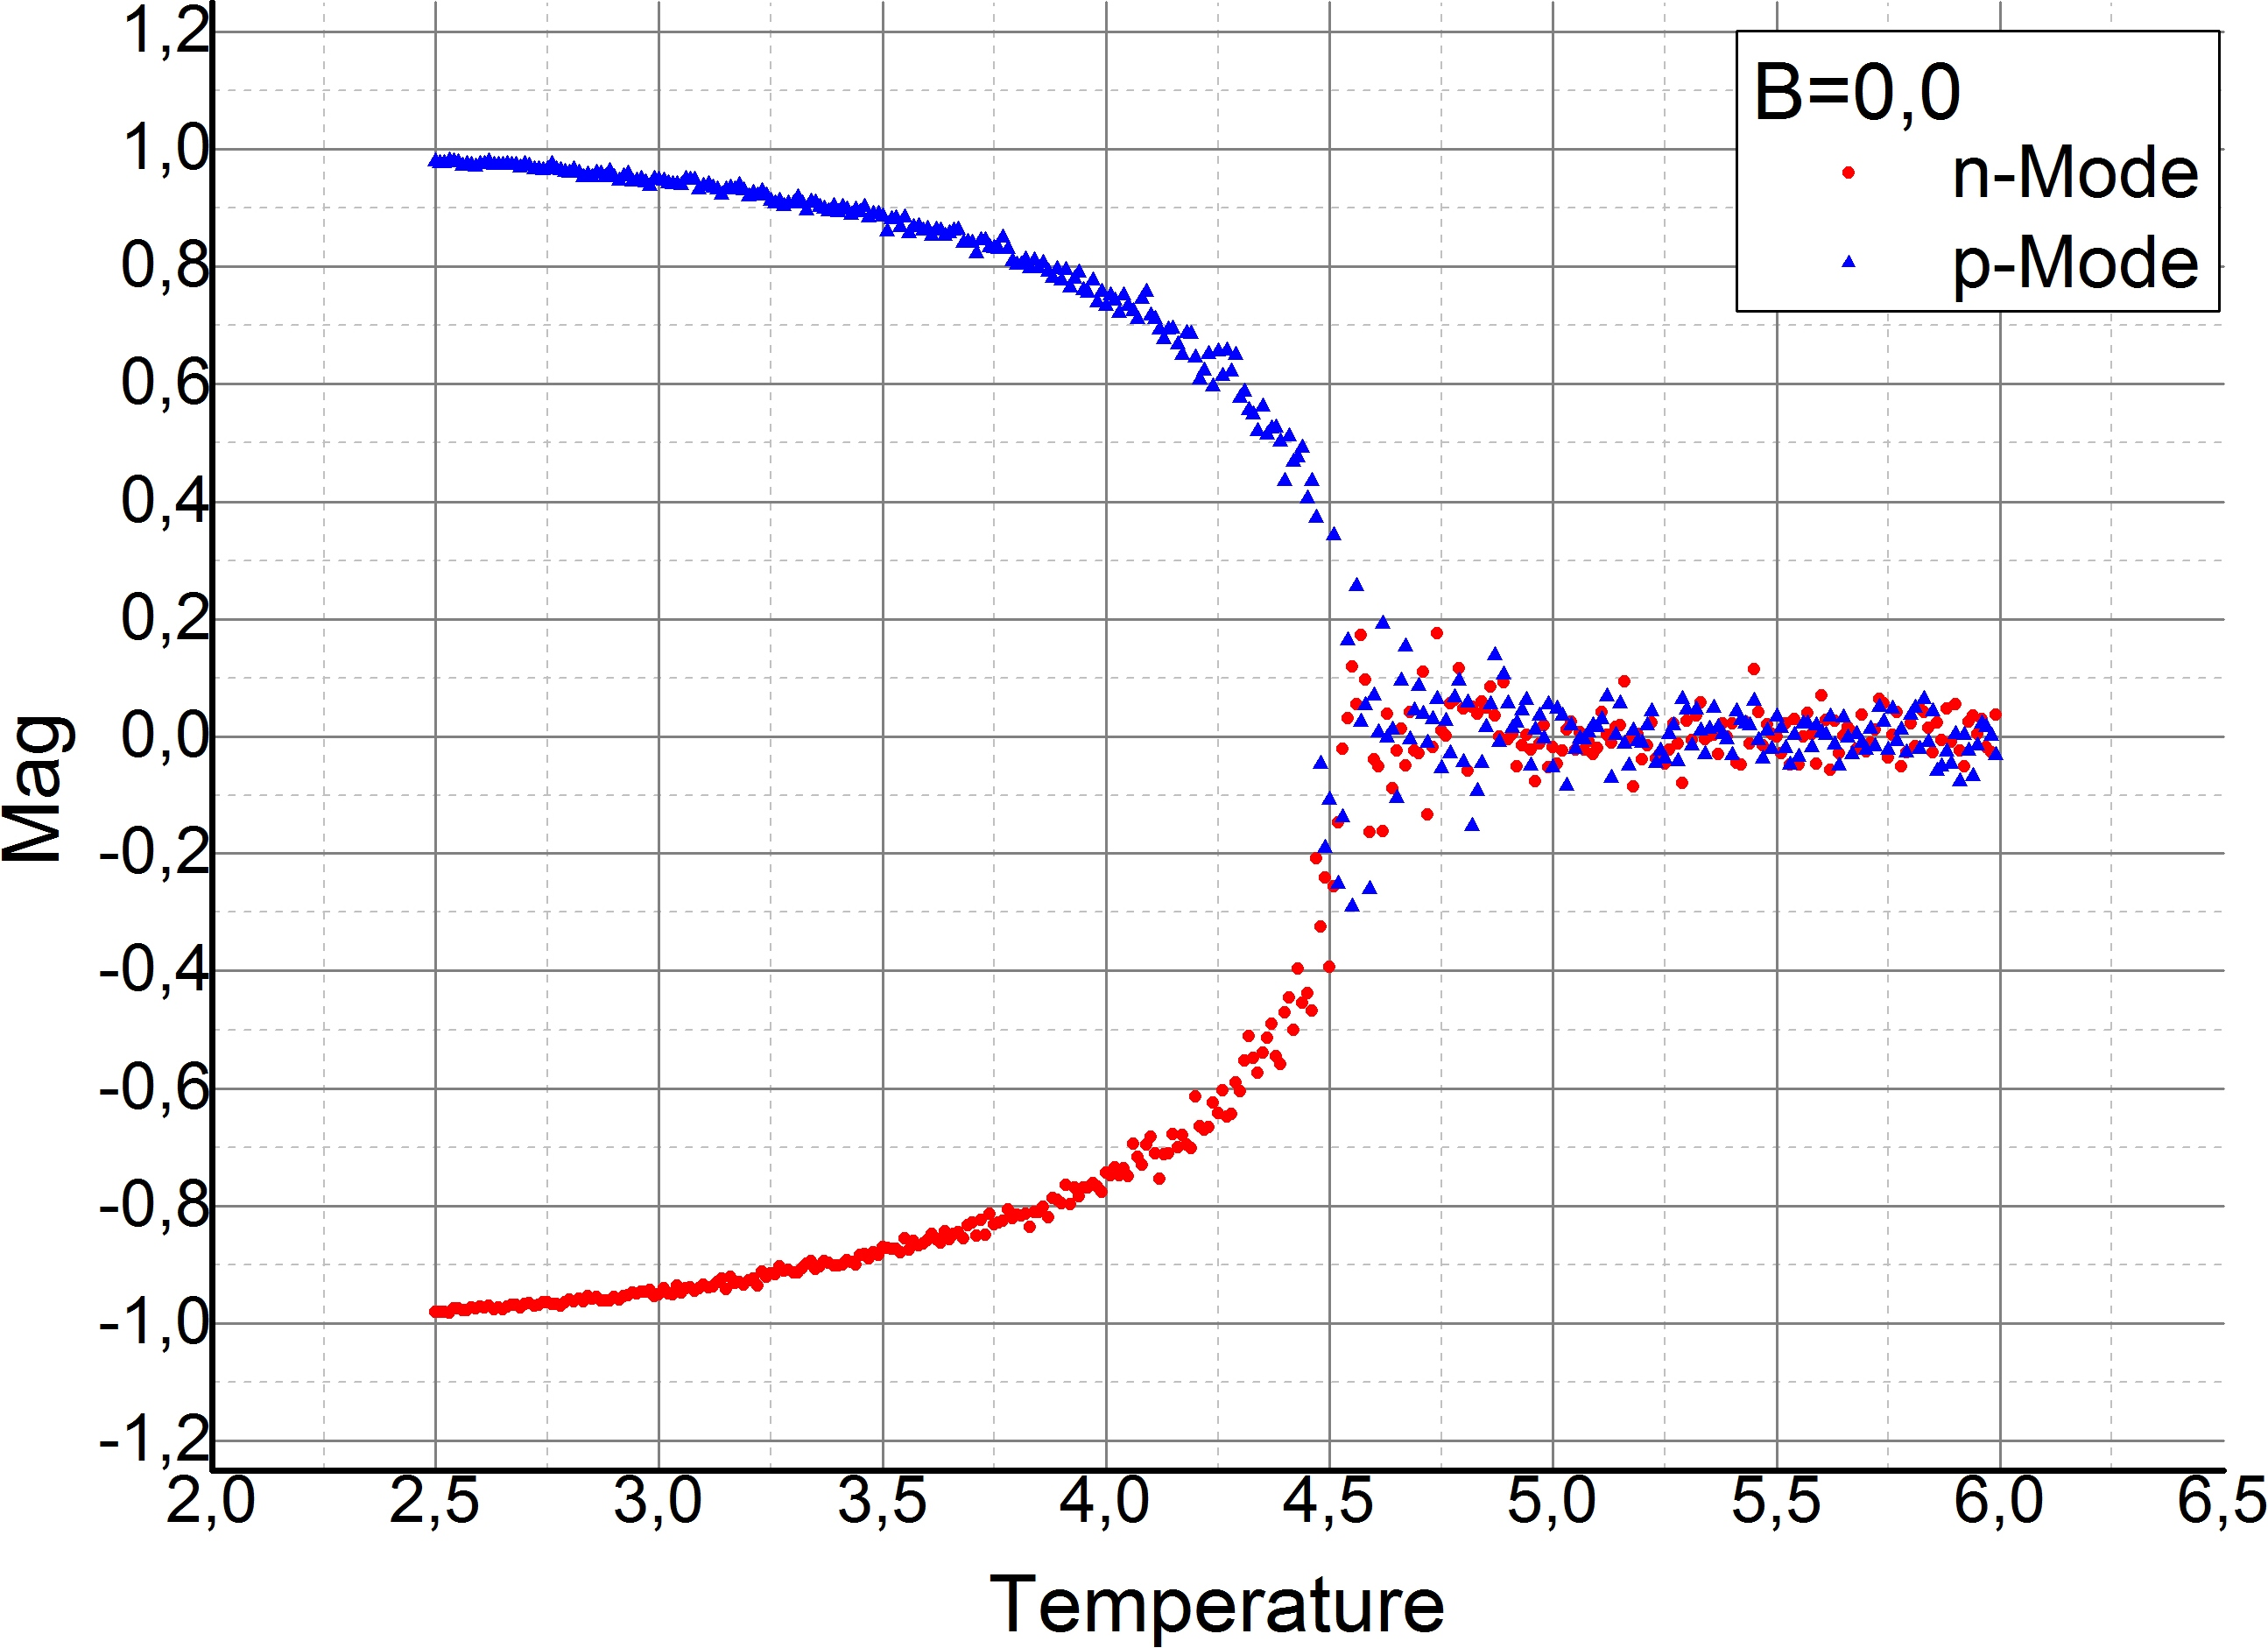
\includegraphics[width=0.47\textwidth]{../Graph_Export/MP3D/m(T)_B=0_pnModes_MP3D_Plot.jpg}
}		
	\caption{Temperaturabhängigkeit der Magnetisierung im 3D Ising Modells via Metropolisalgorithmus ohne äußeres Feld}
	\label{mp3d0modes}
\end{figure}
Zunächst ist erkennbar, dass der grundsätzliche Verlauf mit dem der 2D-Simulation übereinstimmt. Jedoch fällt auf, dass deutlich weniger Ausreißer im Bereich $T<T_{c}$ existieren und auch das Grundrauschen hat deutlich abgenommen. Es liegt nur noch bei etwa $\pm 0,1 = 0,2$. Ersteres liegt vermutlich an der kompakteren Struktur, also der höheren Anzahl an direkten Nachbarn. Zweiteres kommt durch die größere Anzahl an Spins (Gitterpunkten) zustande. Im 3D-Modell ist bei geeigneten Werten die Startkonfiguration auch für Simulationen ohne äußeres Feld zweitrangig. In beiden Fällen kann die Curie-Temperatur mit $T_{c}\approx 4,5\pm 0,02$ abgeschätzt werden.


Auch bei der Untersuchung der Einwirkung verschiedener äußerer Felder treten die gleichen Effekte analog zum 2D-Modell auf. Für die Simulation von $B=\pm 0,1$ wurden Temperaturen von $T=2,5$ bis $T=9,0$ mit Schrittweite $\Delta T= 0,02$ und für $B=\pm 0,4$ Temperaturen von $T=2,5$ bis $T=12,0$ mit Schrittweite $\Delta T= 0,025$ betrachtet (Abb. \ref{mp3db}).
 \begin{figure}[H]
	\centering
	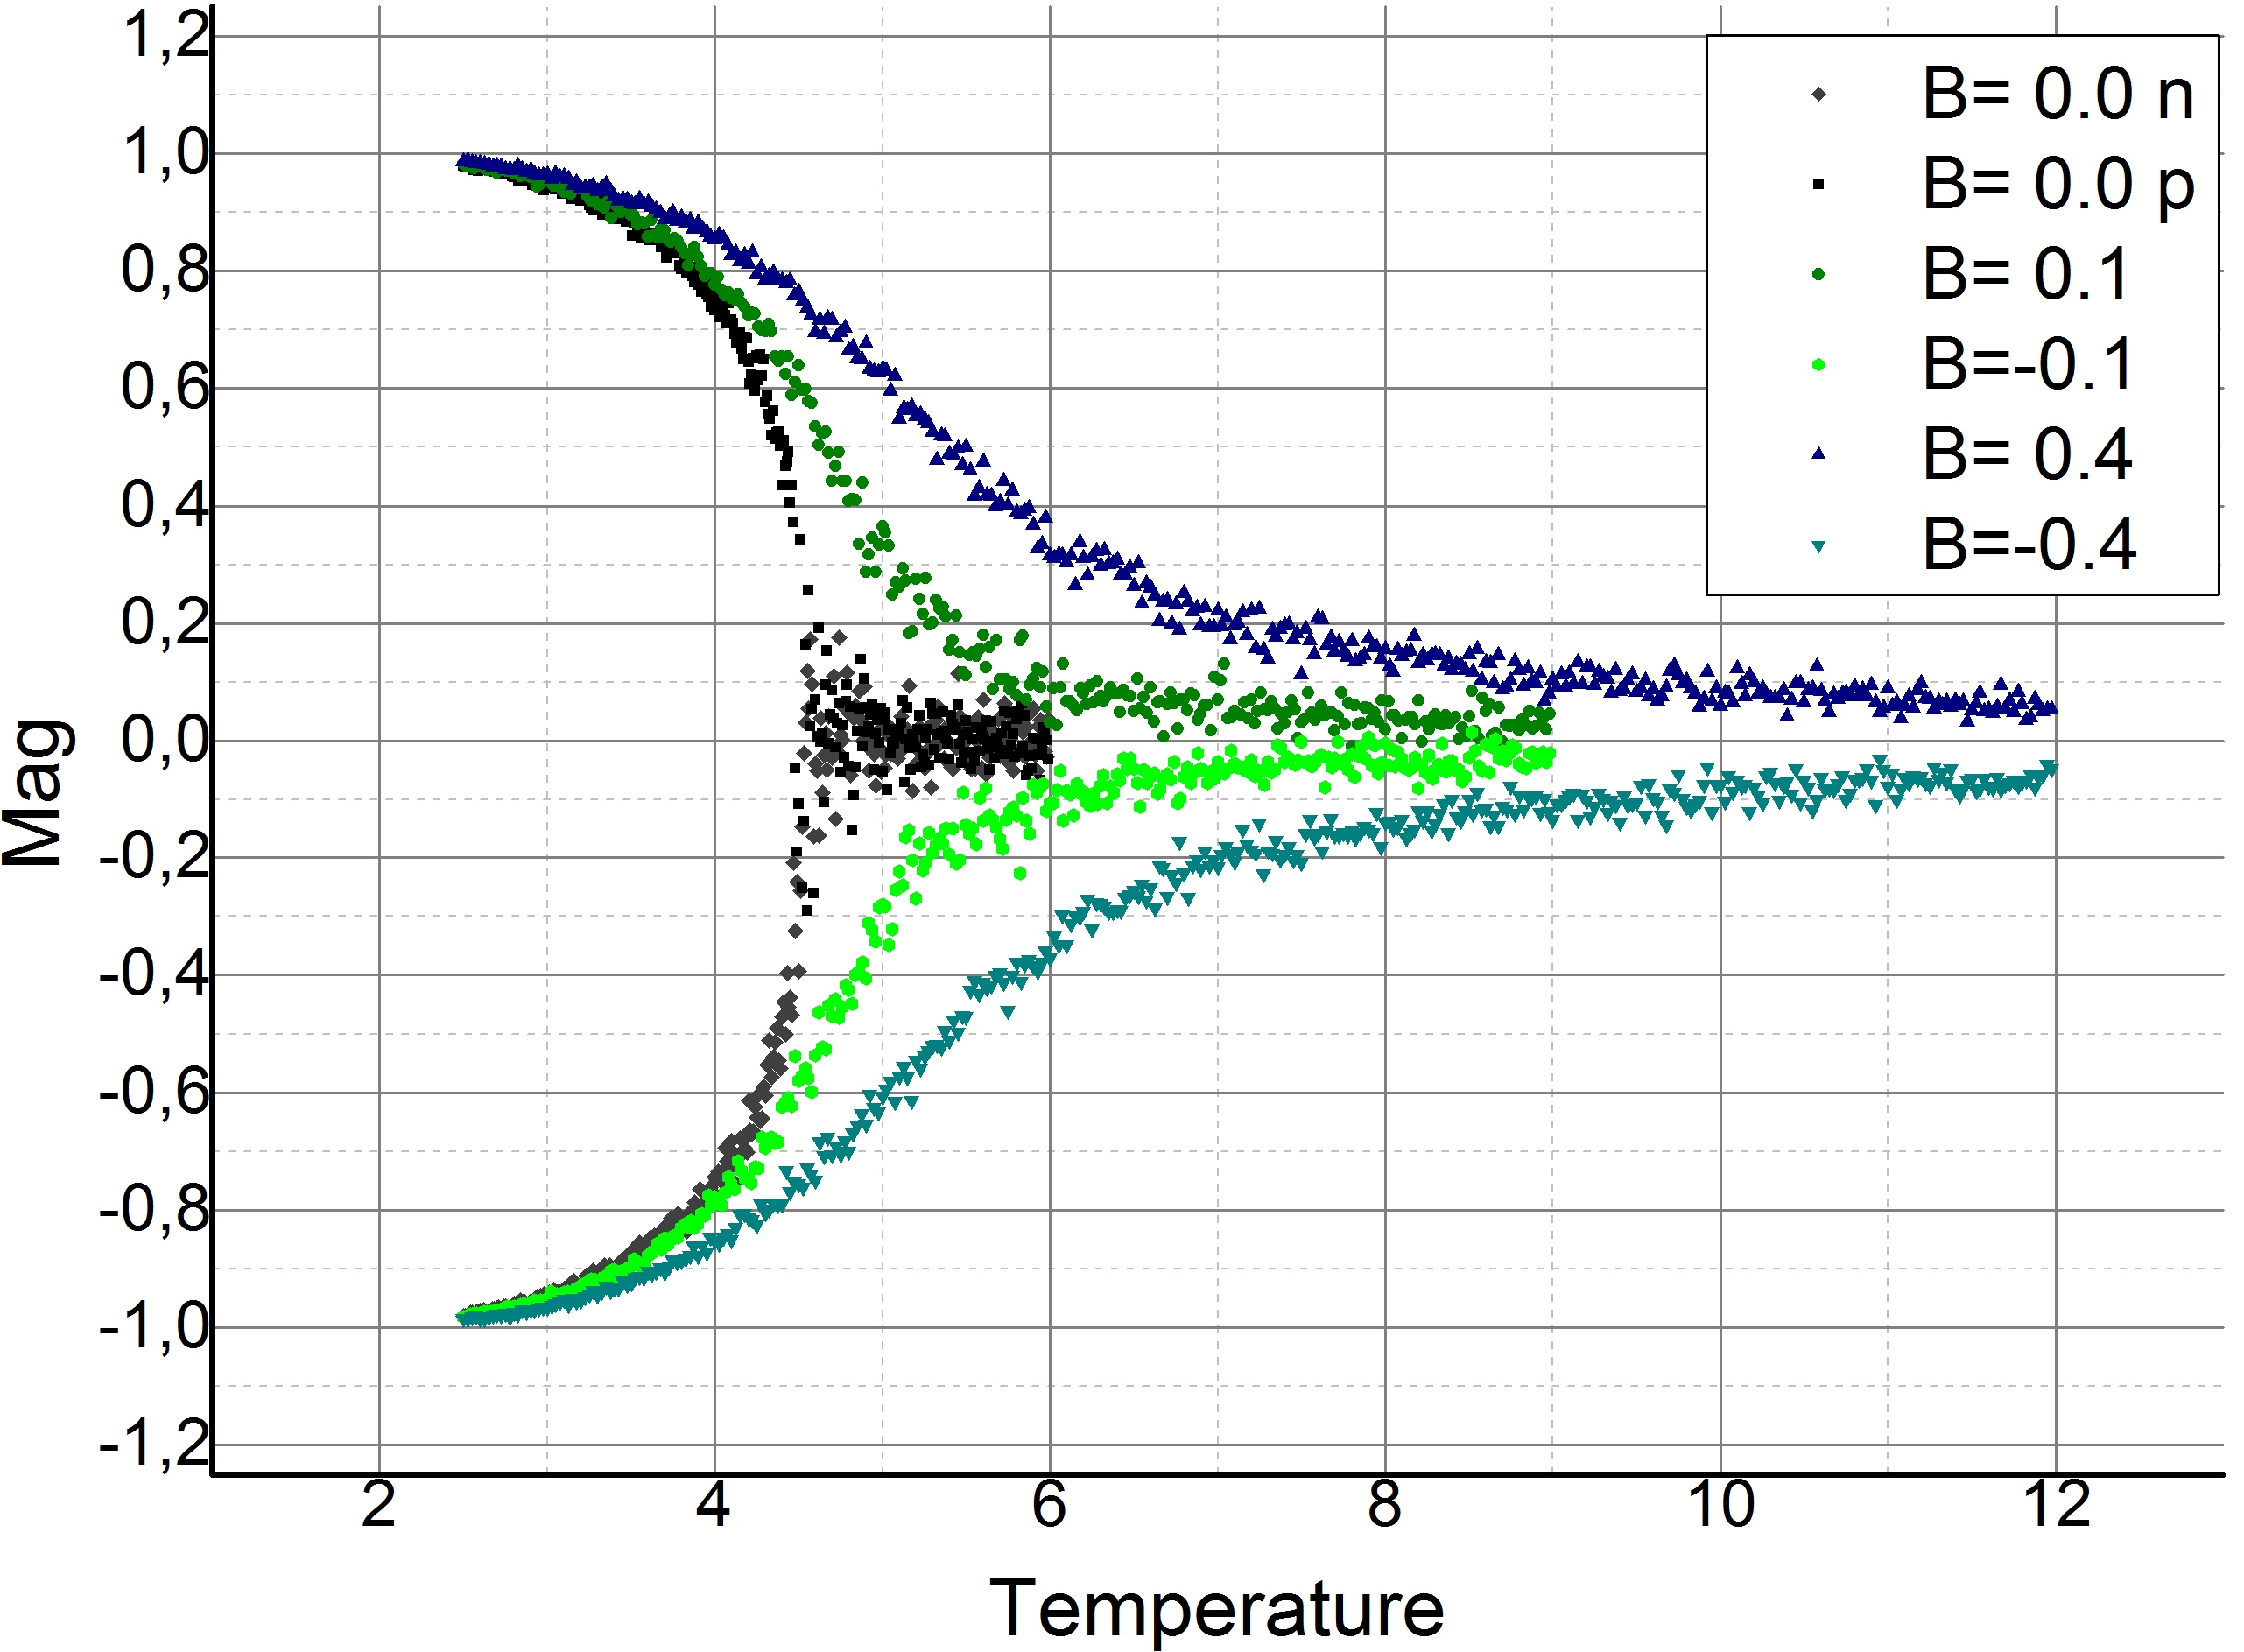
\includegraphics[width=0.8\textwidth]{../Graph_Export/MP3D/m(T)_MP3D_Plot.jpg}	
	\caption{Temperaturabhängigkeit der Magnetisierung im §D Ising Modells via Metropolisalgorithmus für verschiedene äußere Felder}
	\label{mp3db}
\end{figure}


\subsection{Schaltverhalten im Magnetfeld}
\label{auswB}

Als zweites soll die Abhängigkeit der Magnetisierung vom äußeren Feld betrachtet werden. Dies soll Aufschluss über das Schaltverhalten der Magnetisierung für verschiedene Temperaturen liefern. Dazu wird zu Beginn einmal ein Gitter erstellt auf welchem alle Simulationen der verschiedenen Feldstärken hintereinander ausgeführt werden, sodass ein tatsächlicher Sweep des externen Magnetfelds auf einem Gitter simuliert wird. Um das komplette Schaltverhalten zu beobachten, wird der Sweep in beiden Richtungen ausgeführt. Die Ergebnisse für das 2D- und 3D-Modell zeigt Abbildung \ref{mpbsweep}. Hierbei wurde das externe Feld jeweils zwischen $B=\pm1$ bzw $B=\pm1,5$ mit einer Schrittweite von $\Delta B=0,01$ variert. Je Schritt des externen Felds wurde eine Simulation mit 1000 Monte Carlo Schritte ausgeführt. Für die 2D-Simulationen wurde erneut ein 50x50 Gitter und für die 3D-Simulationen ein 20x20x20 Gitter verwendet.
\begin{figure}[H]
	\centering
	\subfigure[2D Modell]{
		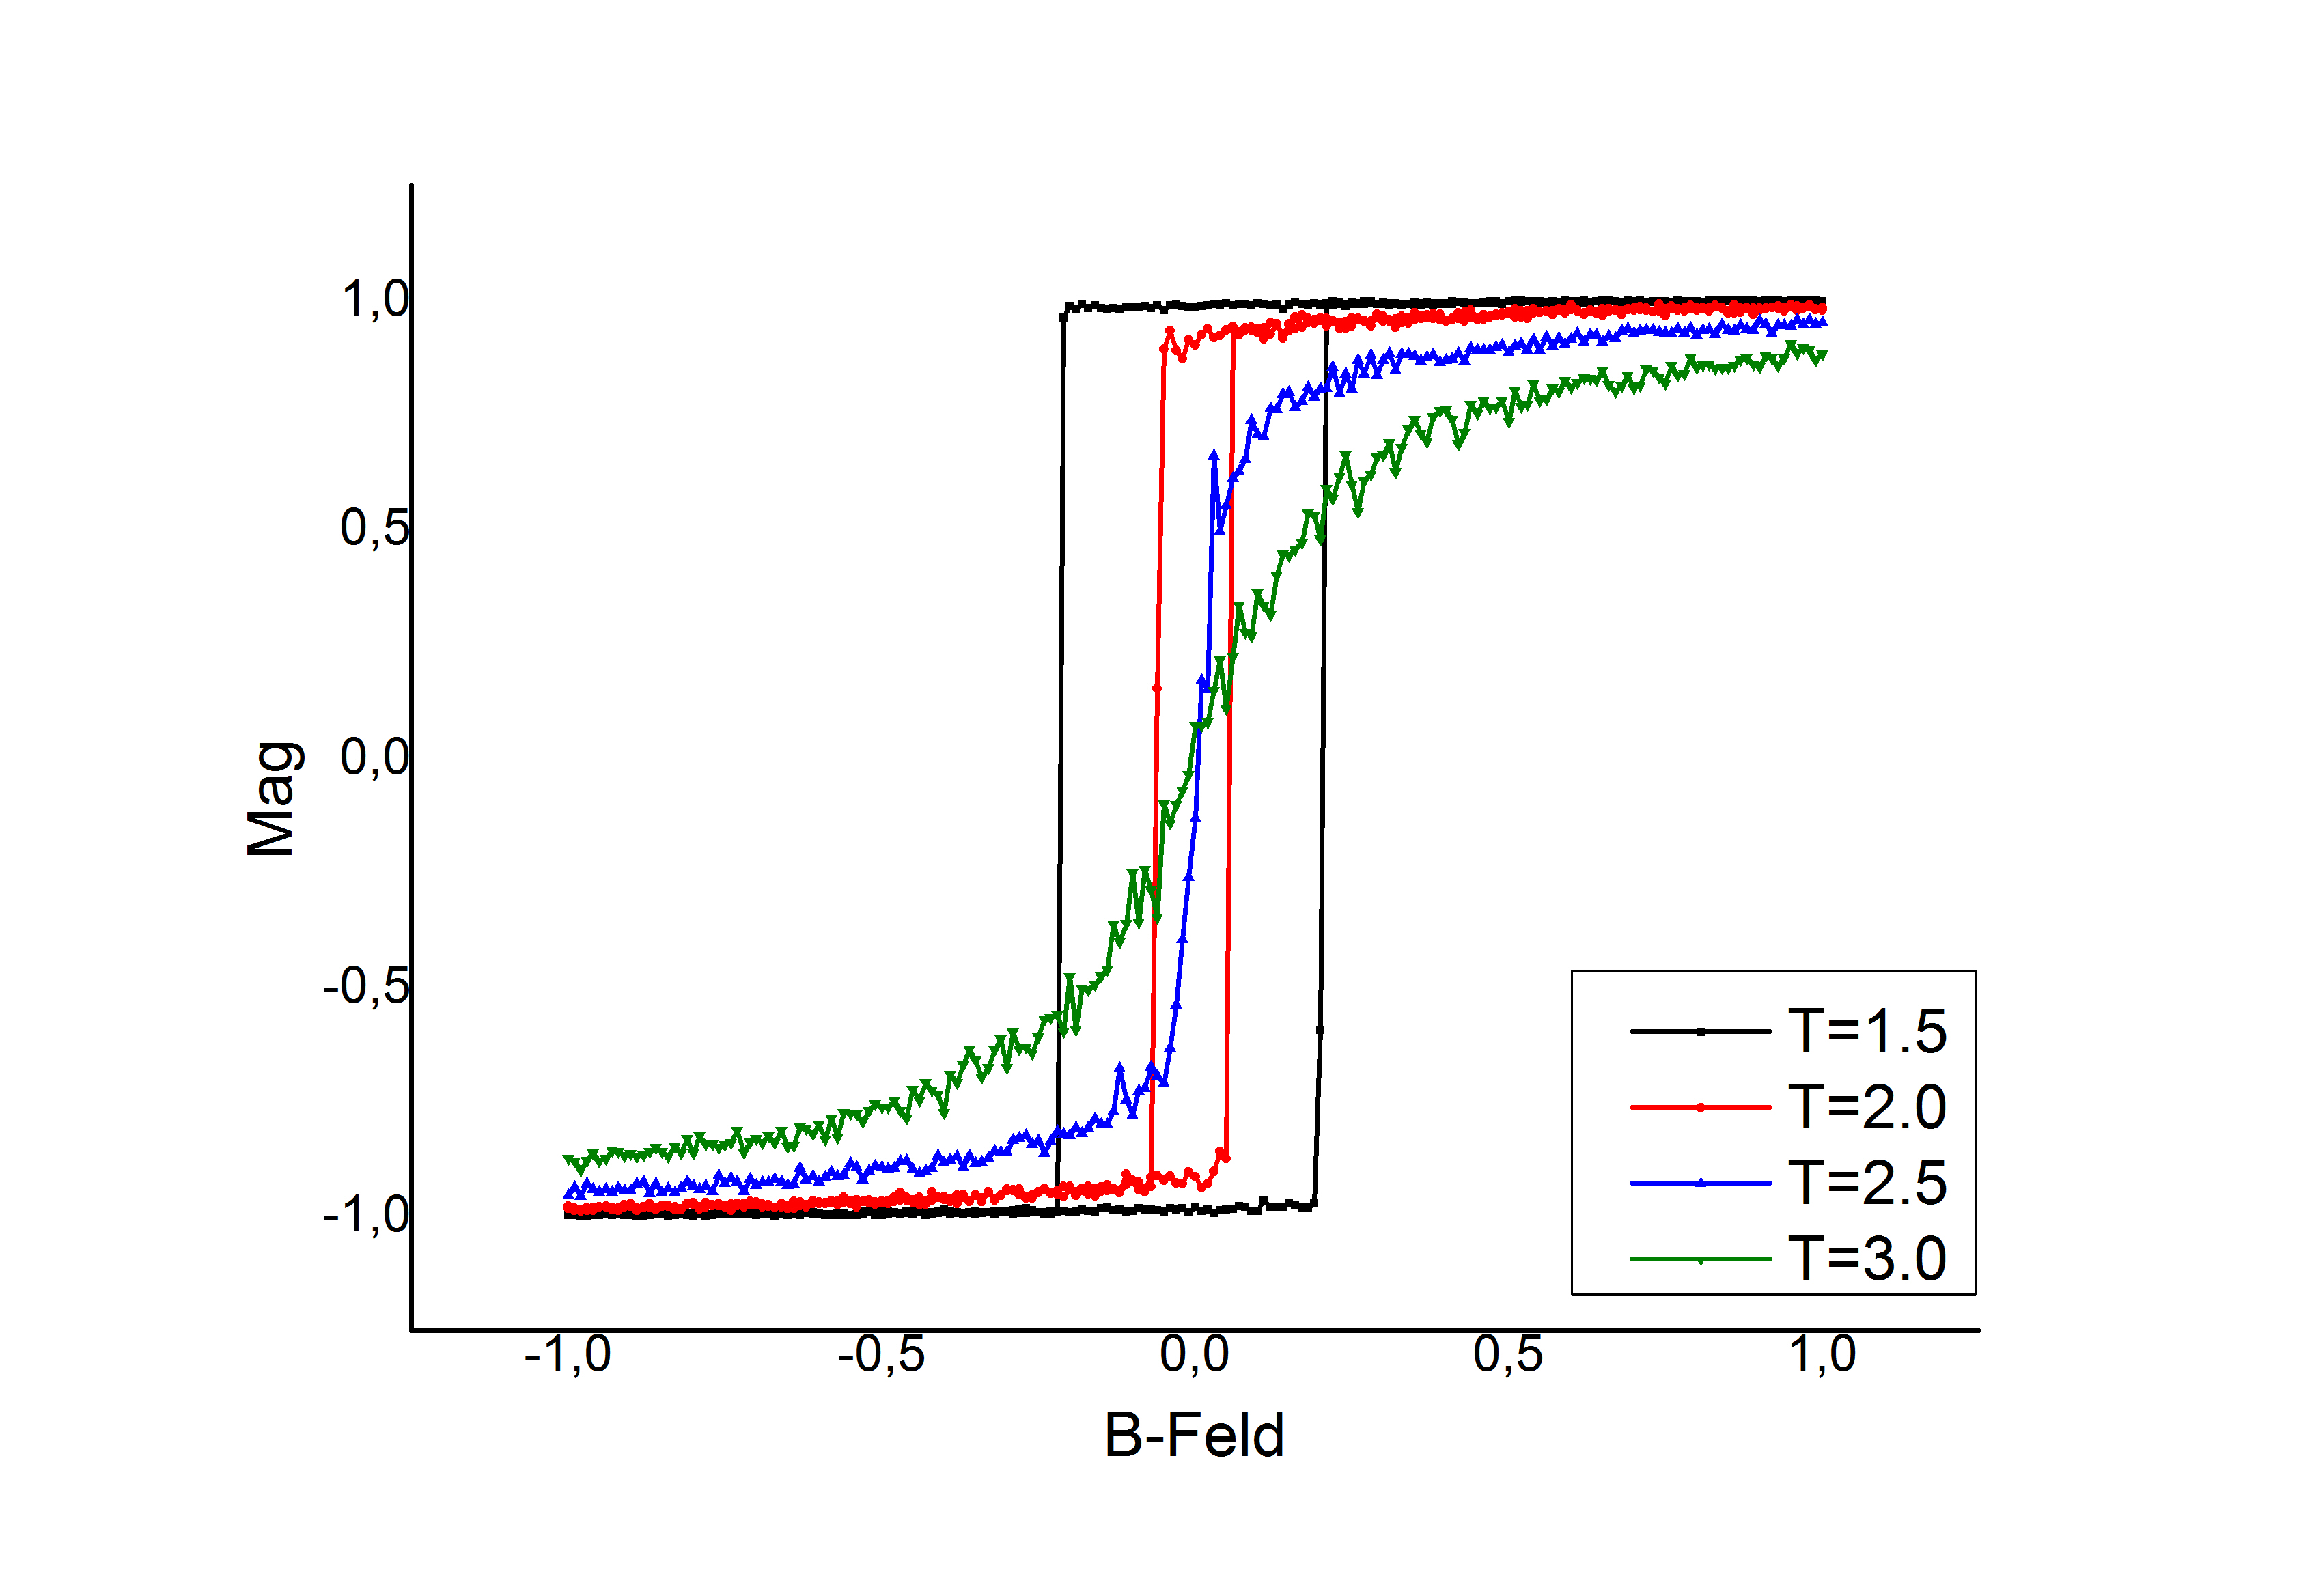
\includegraphics[width=0.47\textwidth]{../Graph_Export/MP2D/m(B)_MP2D_Plot.jpg}
}	
	\subfigure[3D Modell]{
		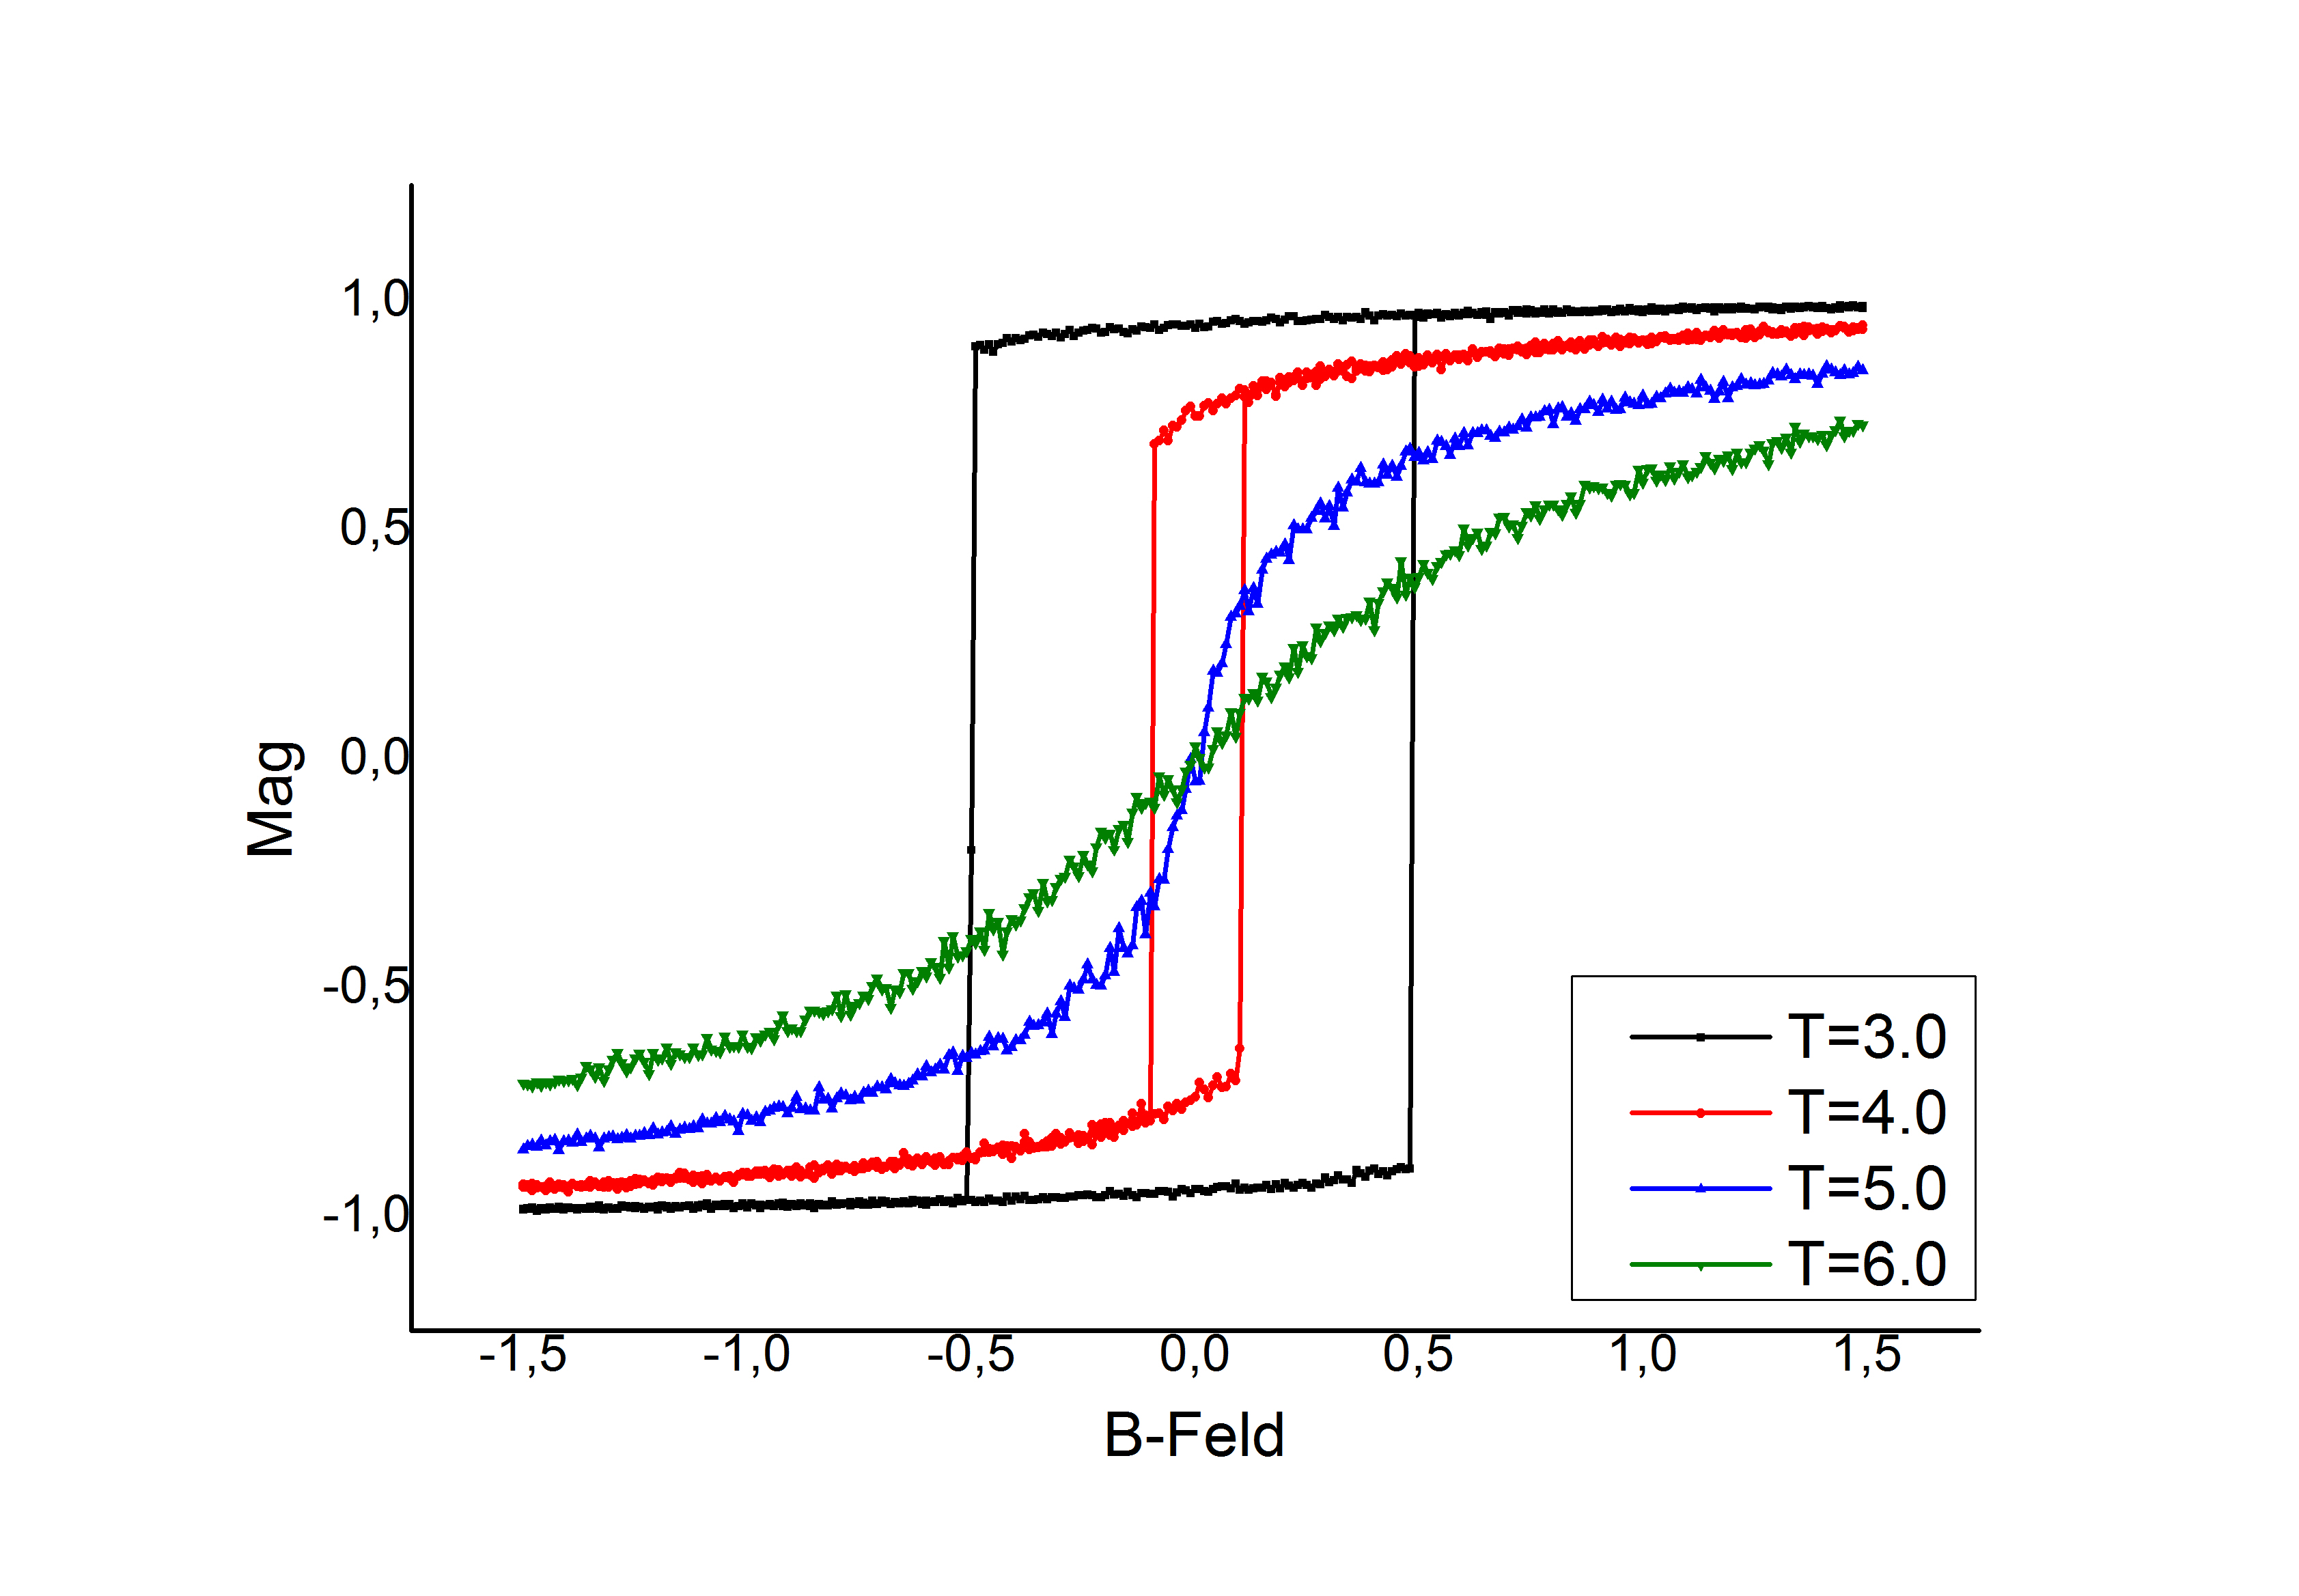
\includegraphics[width=0.47\textwidth]{../Graph_Export/MP3D/m(B)_MP3D_Plot.jpg}
}		
	\caption{Abhängigkeit der Magnetisierung von einem externen Magnetfeld, Simulation via Metropolisalgorithmus auf einem Gitter}
	\label{mpbsweep}
\end{figure}
In beiden Fällen ist zu erkennen, dass sich für $T<T_{c}$ eine Hysterese herausbildet, welche immer schmaler wird, je näher sich $T$ $T_{c}$ annähert. Zudem ist zu beobachten, dass für kleine Temperaturen das Gitter komplett schaltet, währen um $T_{c}$ herum die Magnetiesung vor dem Schalten langsam kolabiert. Dieses Schaltverhalten lässt sich anhand der zwei Minima der freien Energie an $\pm m_{0}$ erklären. Diese liegen je nach Temperatur mehr oder weniger tief, für $B=0$ jedoch auf selber Höhe (Gleichgewicht). Im Falle eines externen Feldes verschiebt sich das Gleichgewicht zu Gunsten des angelegten Feldes. Ein Umschalten findet folglich erst statt, wenn aus dem ungünstigem Extrema ein Wendepunkt geworden ist, was je nach Temperatur bei unterschiedlichen $|B|>0$ der Fall ist (Abb. \ref{fmag}b). An $T_{c}$ selbst ist erstmals keine Hysterese mehr zu erkennen, da ab hier nur noch ein einziges Minimum bei $m=0$ besteht (Abb. \ref{fmag}a). Für $T>T_{c}$ ist ein kontinuierlicher Übergang der Magnetisierung zu beobachten, welcher durch den Ursprung verläuft. Dies deckt sich mit den Ergebnissen der Simulationen zur Temperaturabhängigkeit Kapitel \ref{auswT}. Für höhere Temperaturen ist entsprechend ein stärkeres Feld nötig um eine komplette Magnetisierung zu erreichen. 
\begin{figure}[H]
	\centering
	\subfigure[Temperaturabhängigkeit, $B=0$]{
		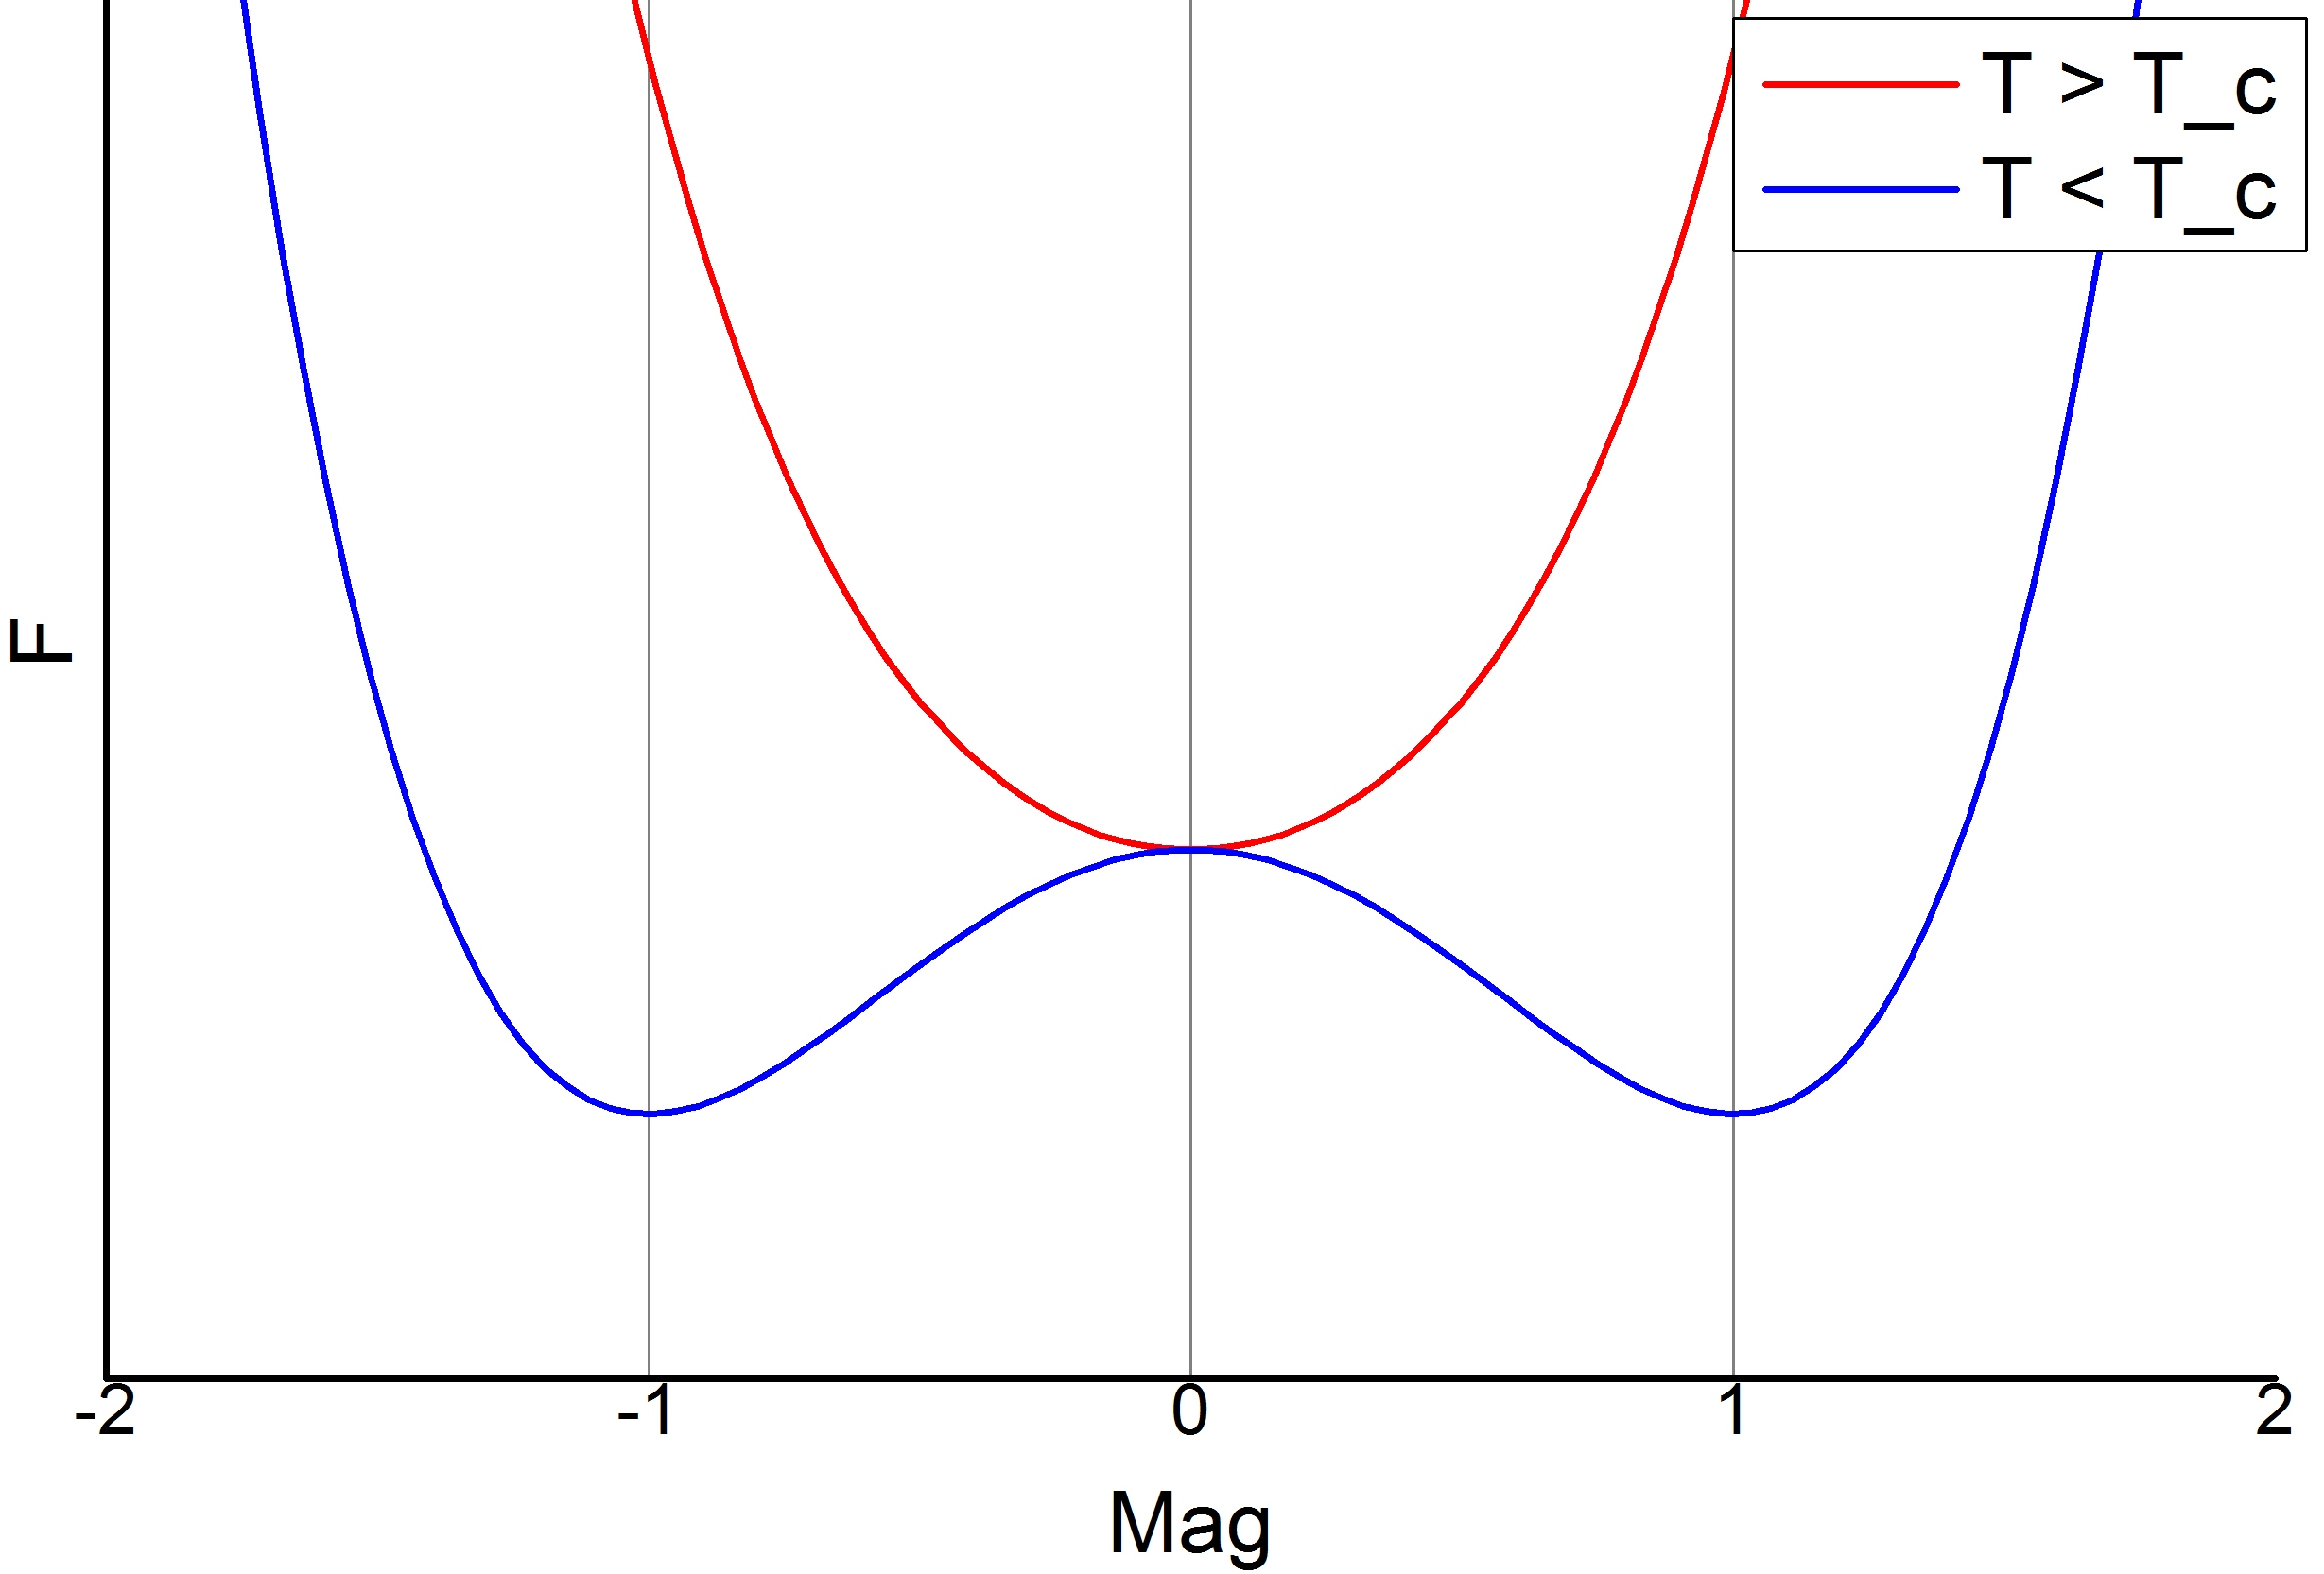
\includegraphics[width=0.35\textwidth]{../Graph_Export/F(mag)_T.jpg}
}	
	\subfigure[Feldabhängigkeit, $T=const.$]{
		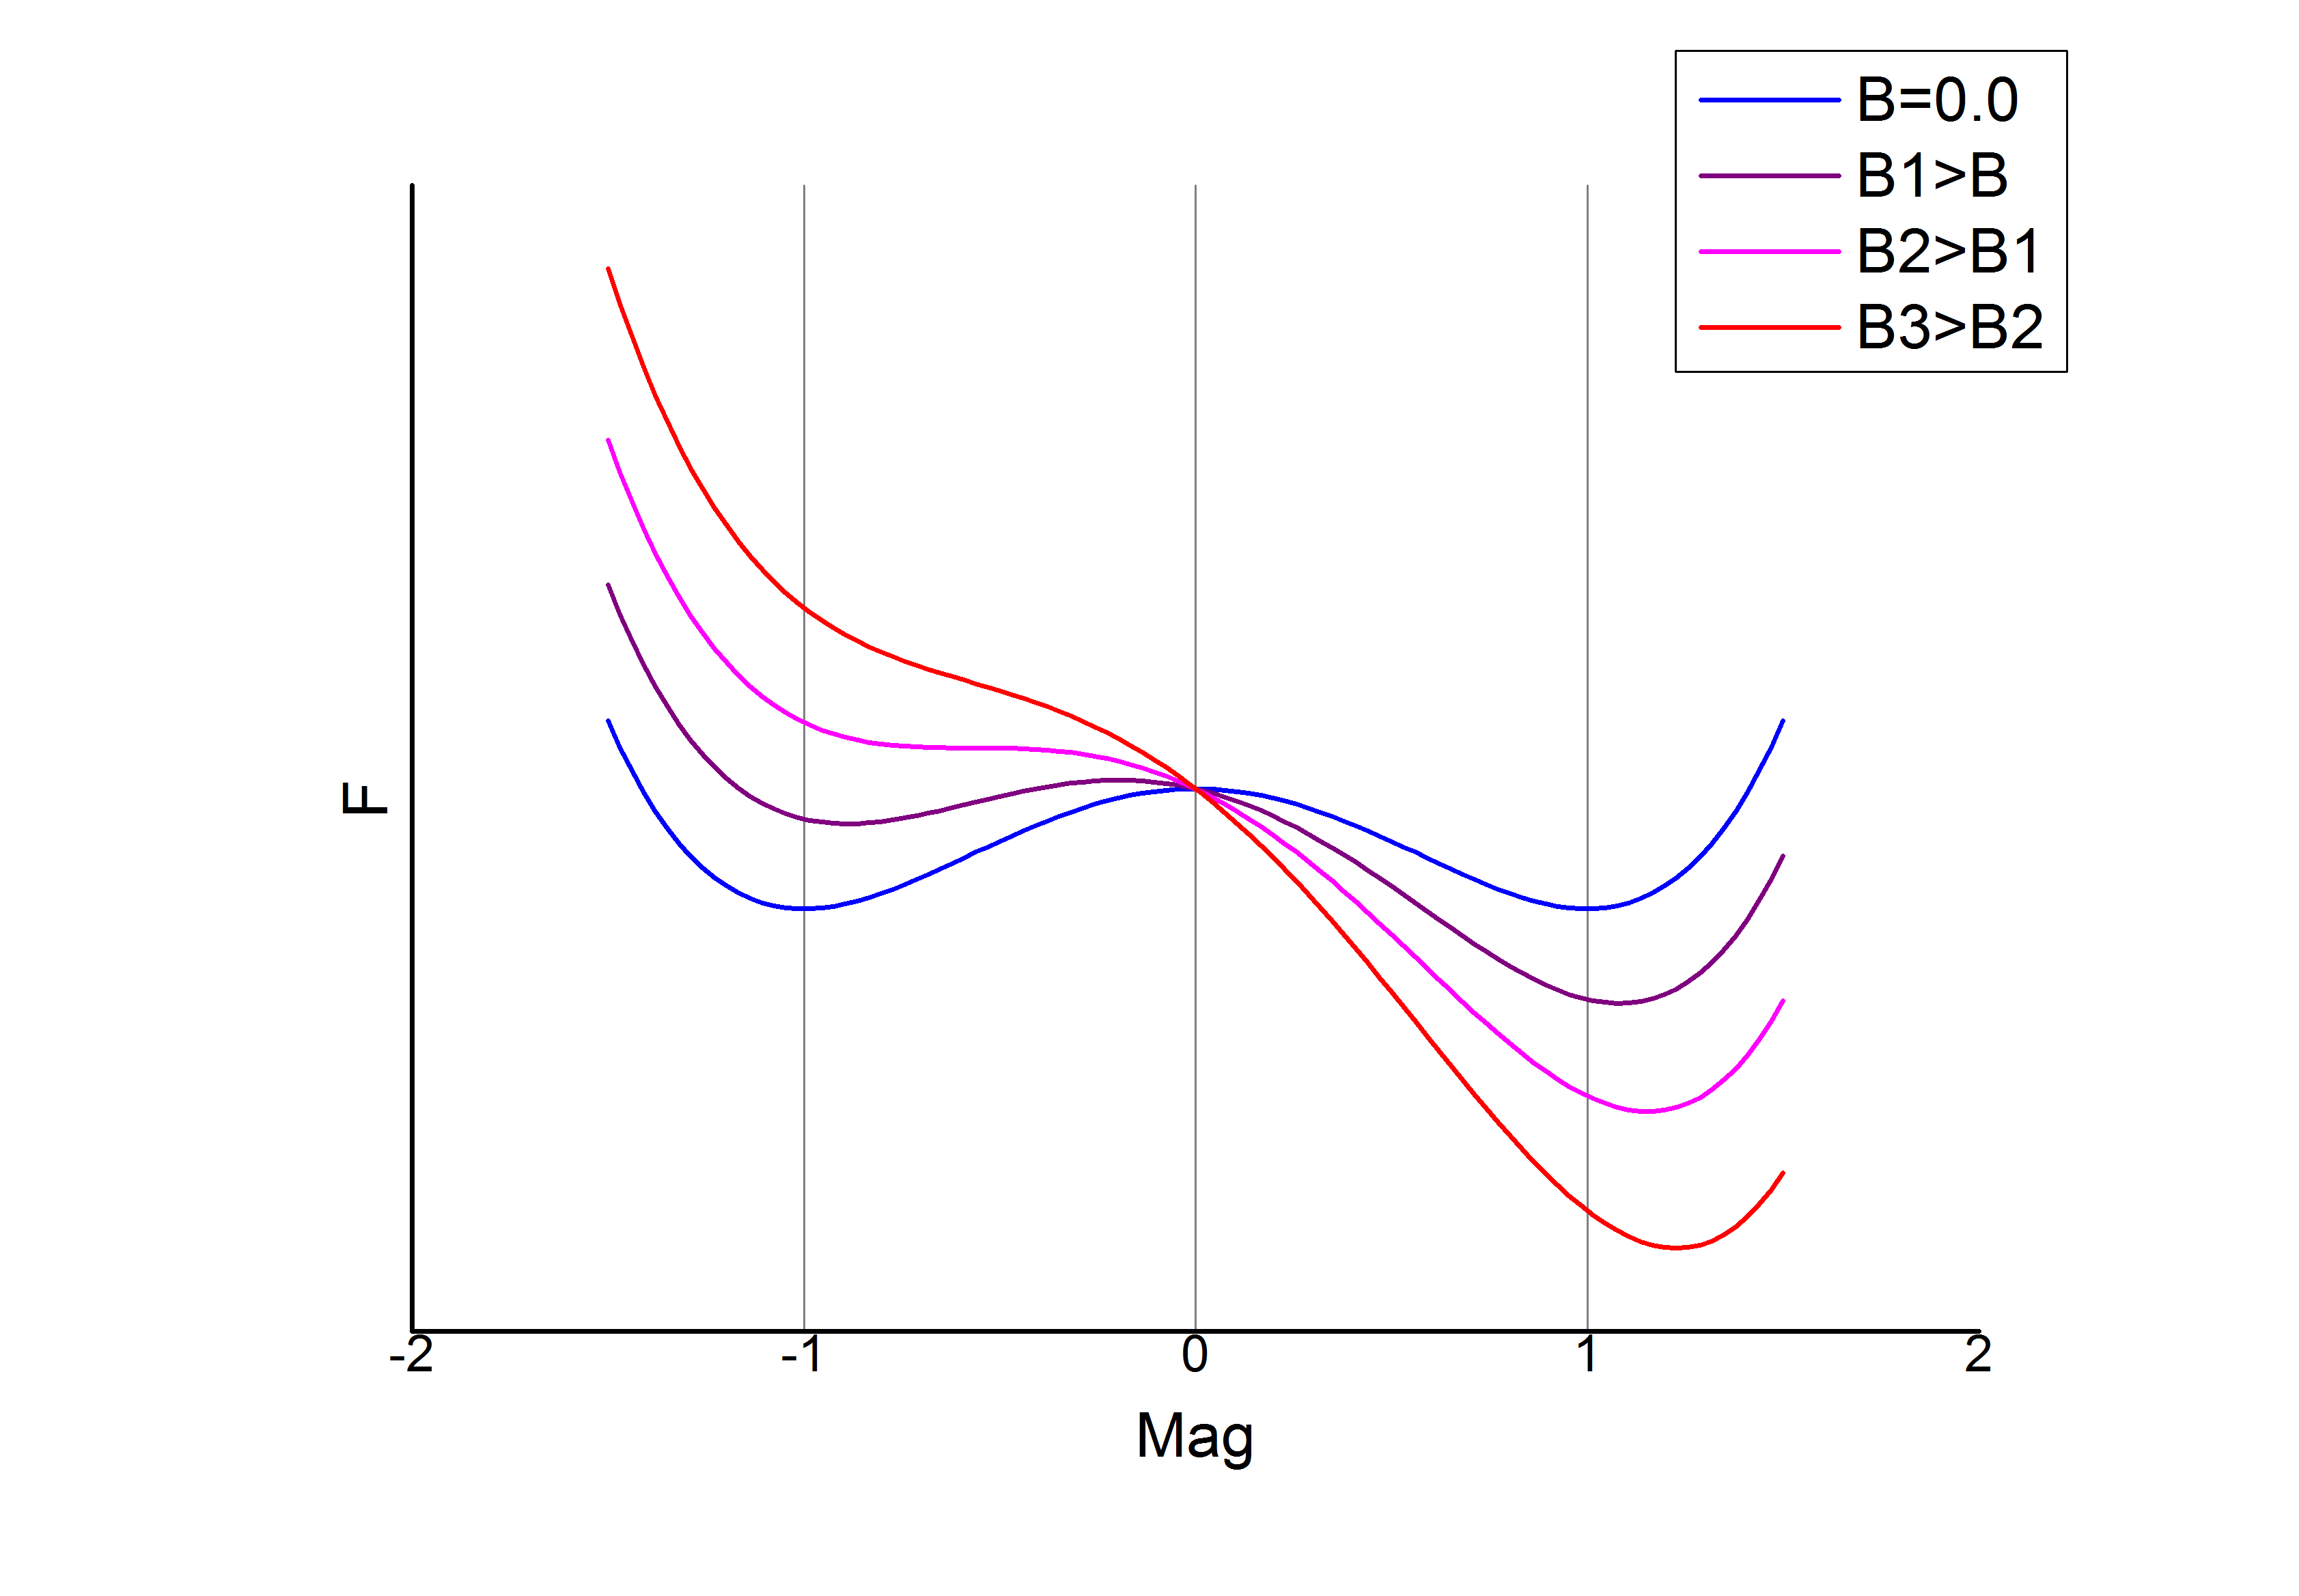
\includegraphics[width=0.35\textwidth]{../Graph_Export/F(mag)_B.jpg}
}		
	\caption{schematischer Verlauf der freien Energie in Abhängigkeit der Magnetisierung. Auswirkung der Temperatur und des externen Magnetfelds}
	\label{fmag}
\end{figure}


\newpage
\section{Alternative: Cluster Monte Carlo Algorithmen}
\label{cluster}
Clusteralgorithmen wirken dem Problem hoher Autokorrelationszeiten im Bereich des Phasenübergangs entgegen.\\
Um dies zu erreichen arbeiten sie nicht mehr nur Lokal, wie der Metropolis Algorithmus, sondern bilden größere Bereiche (Cluster), die auf einmal manipuliert werden.

\subsection{Wolff-Algorithmus}
Der Wolff-Algorithmus ist ein Cluster-Algorithmus, der pro Monte-Carlo-Schritt von einem zufälligen Startpunkt aus ein Cluster bildet und dann mit einer bestimmten Wahrscheinlichkeit alle Spins innerhalb des Clusters flippt.\\\\
Allgemeiner Programmablauf:\\
1. Startkonfiguration (Abbildung \ref{cu2veransch}a)\\
2. Bestimmte einen zufälligen Startpunkt (Abbildung \ref{cu2veransch}b)\\
3. Ausgehend vom Startpunkt werden benachbarte Atome mit gleichem Spin mit Wahrscheinlichkeit p in den Cluster aufgenommen (Abbildung \ref{cu2veransch}c,d,e)\\
4. Flippe alle Spins des Clusters mit einer Wahrscheinlichkeit (Abbildung \ref{cu2veransch}f)\\
5. Gehe zu 1.\\
\begin{figure}[H]
	\centering
	\subfigure[]{
		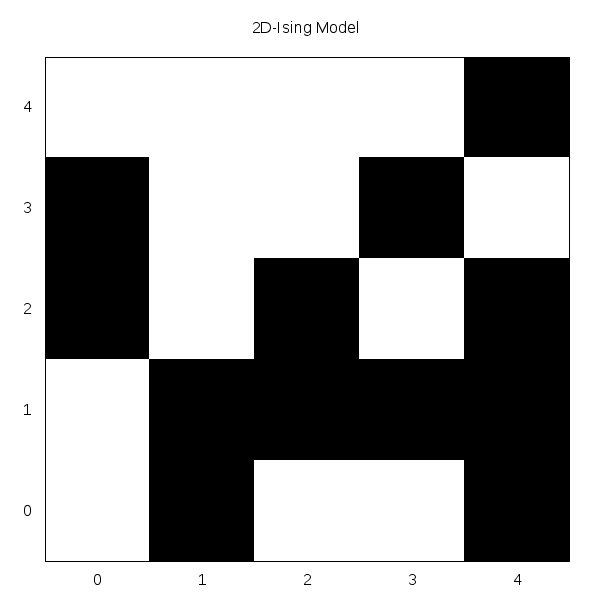
\includegraphics[width=0.25\textwidth]{../Graph_Export/cluster_veranschaulichung/Abbildung41.png}
	}
	\subfigure[]{
		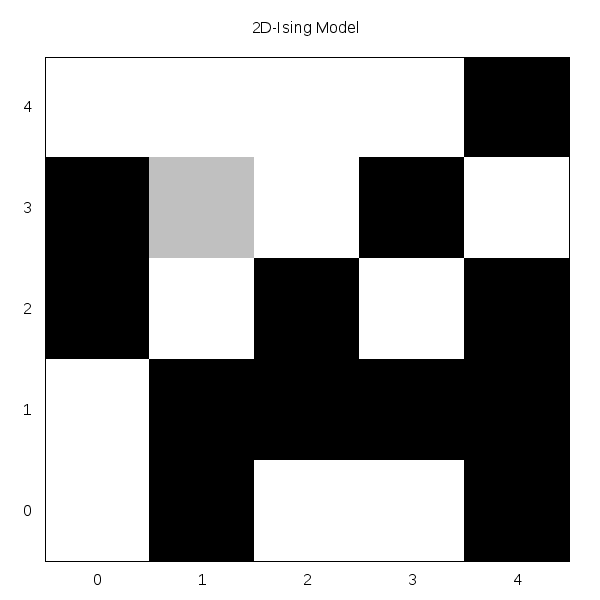
\includegraphics[width=0.25\textwidth]{../Graph_Export/cluster_veranschaulichung/Abbildung42.png}
	}
	\subfigure[]{
		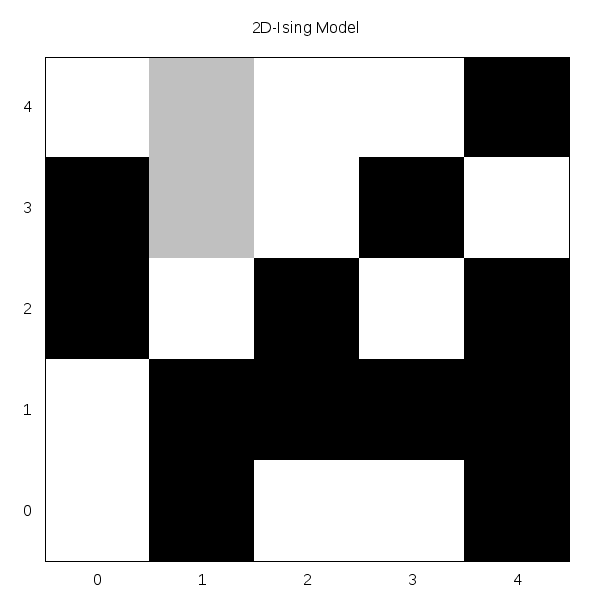
\includegraphics[width=0.25\textwidth]{../Graph_Export/cluster_veranschaulichung/Abbildung43a.png}
	}
	\subfigure[]{
		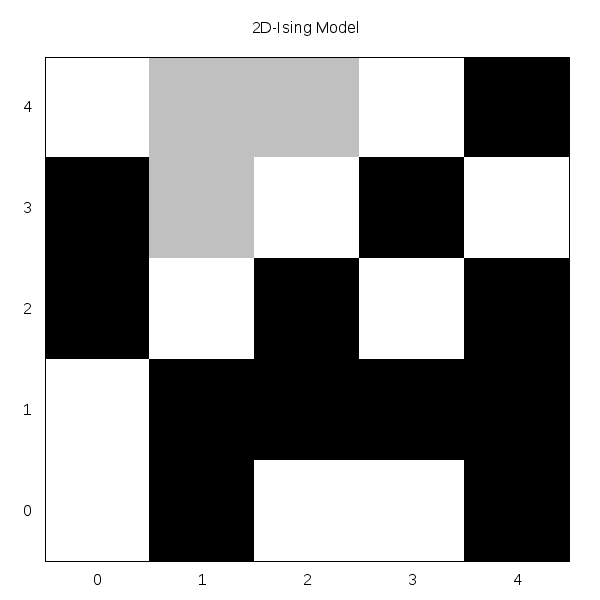
\includegraphics[width=0.25\textwidth]{../Graph_Export/cluster_veranschaulichung/Abbildung43b.png}
	}
	\subfigure[]{
		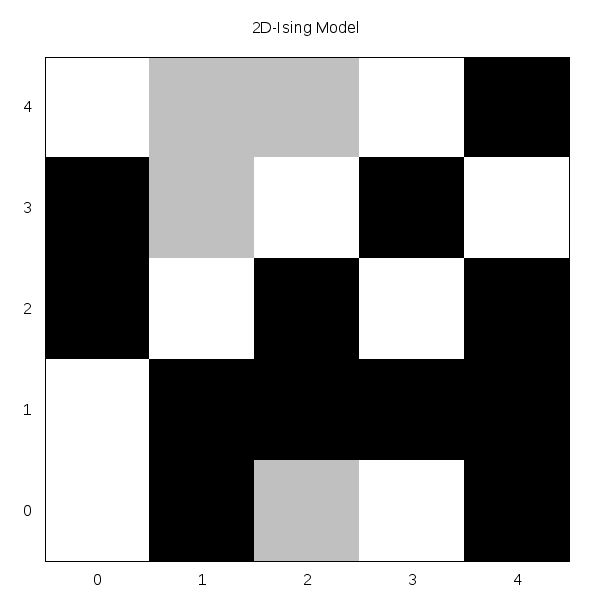
\includegraphics[width=0.25\textwidth]{../Graph_Export/cluster_veranschaulichung/Abbildung43c.png}
	}
	\subfigure[]{
		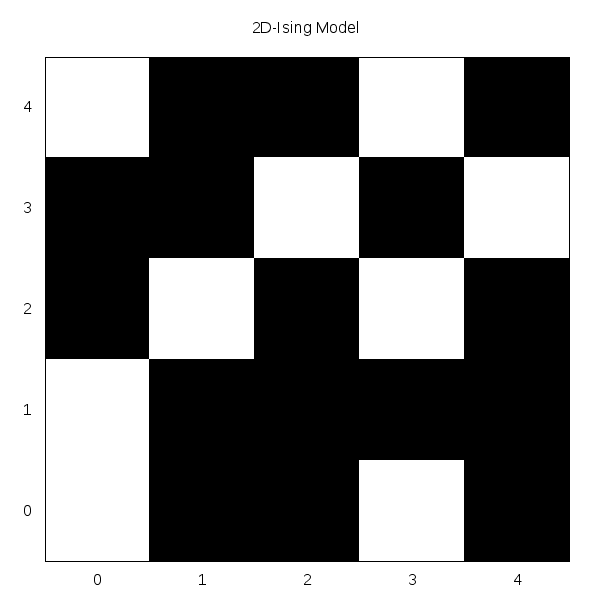
\includegraphics[width=0.25\textwidth]{../Graph_Export/cluster_veranschaulichung/Abbildung44.png}
	}
	\caption{Veranschaulichung des Wolff-Algorithmus Schemas}
	\label{cu2veransch}
\end{figure}


\subsection{Flipp-Wahrscheinlichkeit des Clusters = 1}
Der Algorithmus wird besonders effizient, da bei einer bestimmten Annahme-Wahrscheinlichkeit p, dass ein Zustand in den Cluster aufgenommen wird, der Cluster in jedem Monte-Carlo-Schritt geflippt wird.\\\\
Warum dies so ist wird klar, wenn man sich die Wahrscheinlichkeit $W_{ij}$ für den Übergang von der Konfiguration i zu j berechnet.
\begin{align}
W_{ij} = min\{1, \frac{A(j \rightarrow i) * P_j}{A(i \rightarrow j) * P_i} \} = min\{1, \frac{A(j \rightarrow i) * e^{-\beta E_j}}{A(i \rightarrow j) * e^{-\beta E_i}} \}
\end{align}
Für die Wahrscheinlichkeit $A(i \rightarrow j)$ den Übergang von i nach j zu betrachten und für die Energie $E_i$ im Zustand i gelten:\\
(Hierbei bedeutet $_{innen}$ jeweils innerhalb und $_{außen}$ außerhalb des Clusters\\
und $n_{gleich}$ bzw. $n_{diff}$ sind die Anzahl Spins, die am Rand gleich bzw. ungleich zu dem Spin innerhalb des Clusters sind.)
\begin{align}
A(i \rightarrow j)=A_{innen} * (1 - p)^{n_{gleich}}\\
A_{innen} = p^{n_{innen}-1} + Z\\
E_i = E_{innen} + E_{außen} - n_{gleich} * J + n_{diff} * J\\
\end{align}
Mit Z der Wahrscheinlichkeit einen Spin im Cluster als Startpunkt gewählt zu haben.\\
Ebenso gilt:
\begin{align}
A(j \rightarrow i)=A_{innen} * (1 - p)^{n_{diff}}\\
E_j = E_{innen} + E_{außen} + n_{gleich} * J - n_{diff} * J\\
\end{align}
Damit gilt:
\begin{align}
W_{ij} &= min\{1, \frac{A_{innen}*(1-p)^{n_{diff}}}{A_{innen}*(1-p)^{n_{gleich}}} * \frac{e^{-\beta E_{innen} + E_{außen} + n_{gleich} * J - n_{diff} * J}}{e^{-\beta E_{innen} + E_{außen} - n_{gleich} * J + n_{diff} * J}}\} \\
&= min\{1, \frac{(1-p)^{n_{diff}}}{(1-p)^{n_{gleich}}} * \frac{e^{-\beta n_{gleich} * J} * e^{+\beta n_{diff} * J}}{e^{+\beta n_{gleich} * J} * e^{-\beta n_{diff} * J}}\}\\
&= min\{1, \frac{(1-p)^{n_{diff}}}{(1-p)^{n_{gleich}}} * \frac{e^{-2\beta n_{gleich} * J}}{e^{-2\beta n_{diff} * J}}\}\\
&= min\{1, \left(\frac{(1-p)}{e^{-2\beta J}}\right)^{n_{diff}} * \left(\frac{e^{-2\beta J}}{(1-p)}\right)^{n_{gleich}}\}
\end{align}
Hieraus lässt sich nun erkennen, dass die Wahrscheinlichkeit vom Zustand i zu j überzugehen gleich $1$ wird, wenn wir $p = 1 - e^{-2\beta J}$ wählen.

\subsection{Metropolis und Cluster-Update im Vergleich}
Der Vorteil des Cluster-Algorithmus ist die schnelle Konverenzgeschwindigkeit in der Nähe des Phasenübergangs bzw. der kritischen Temperatur.\\\\

\begin{figure}[H]
	\centering
	\subfigure[Konvergenz beim Cluster-Update-Verfahren]{
		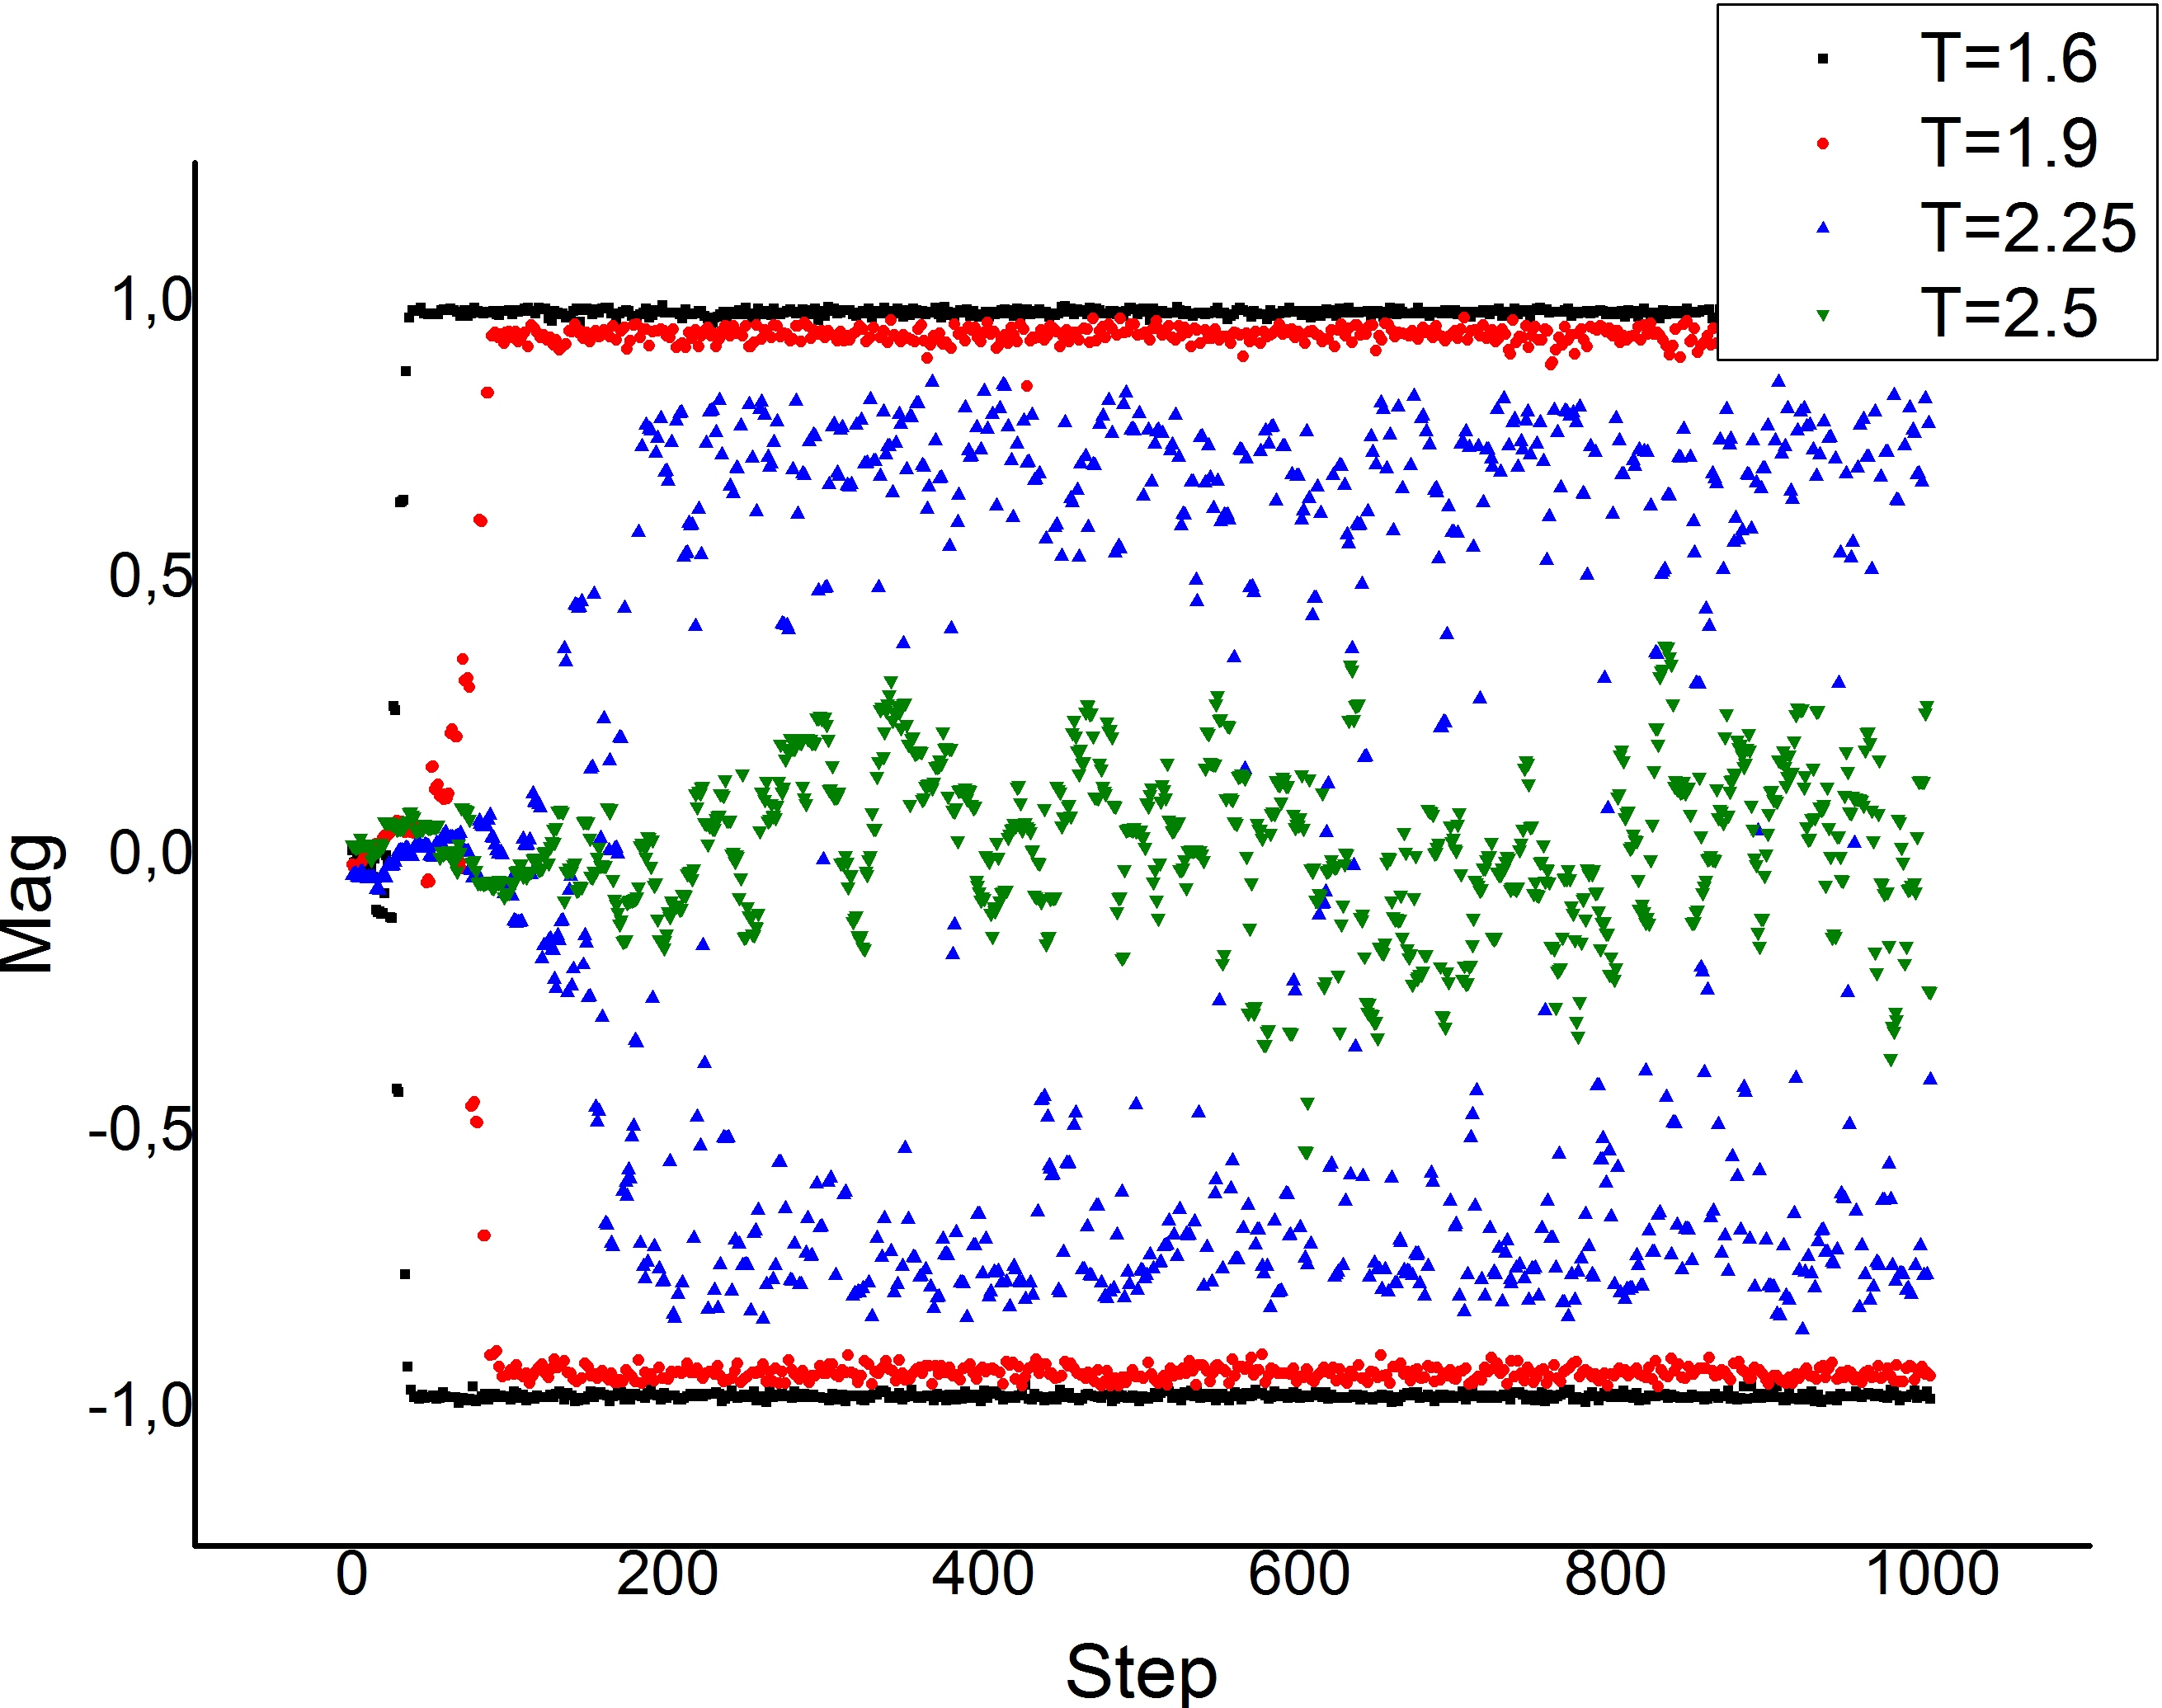
\includegraphics[width=0.30\textwidth]{../Graph_Export/CU2D/m(steps)_Plot.jpg}
	}
	\subfigure[Betragswerte der Abbildung (a)]{
		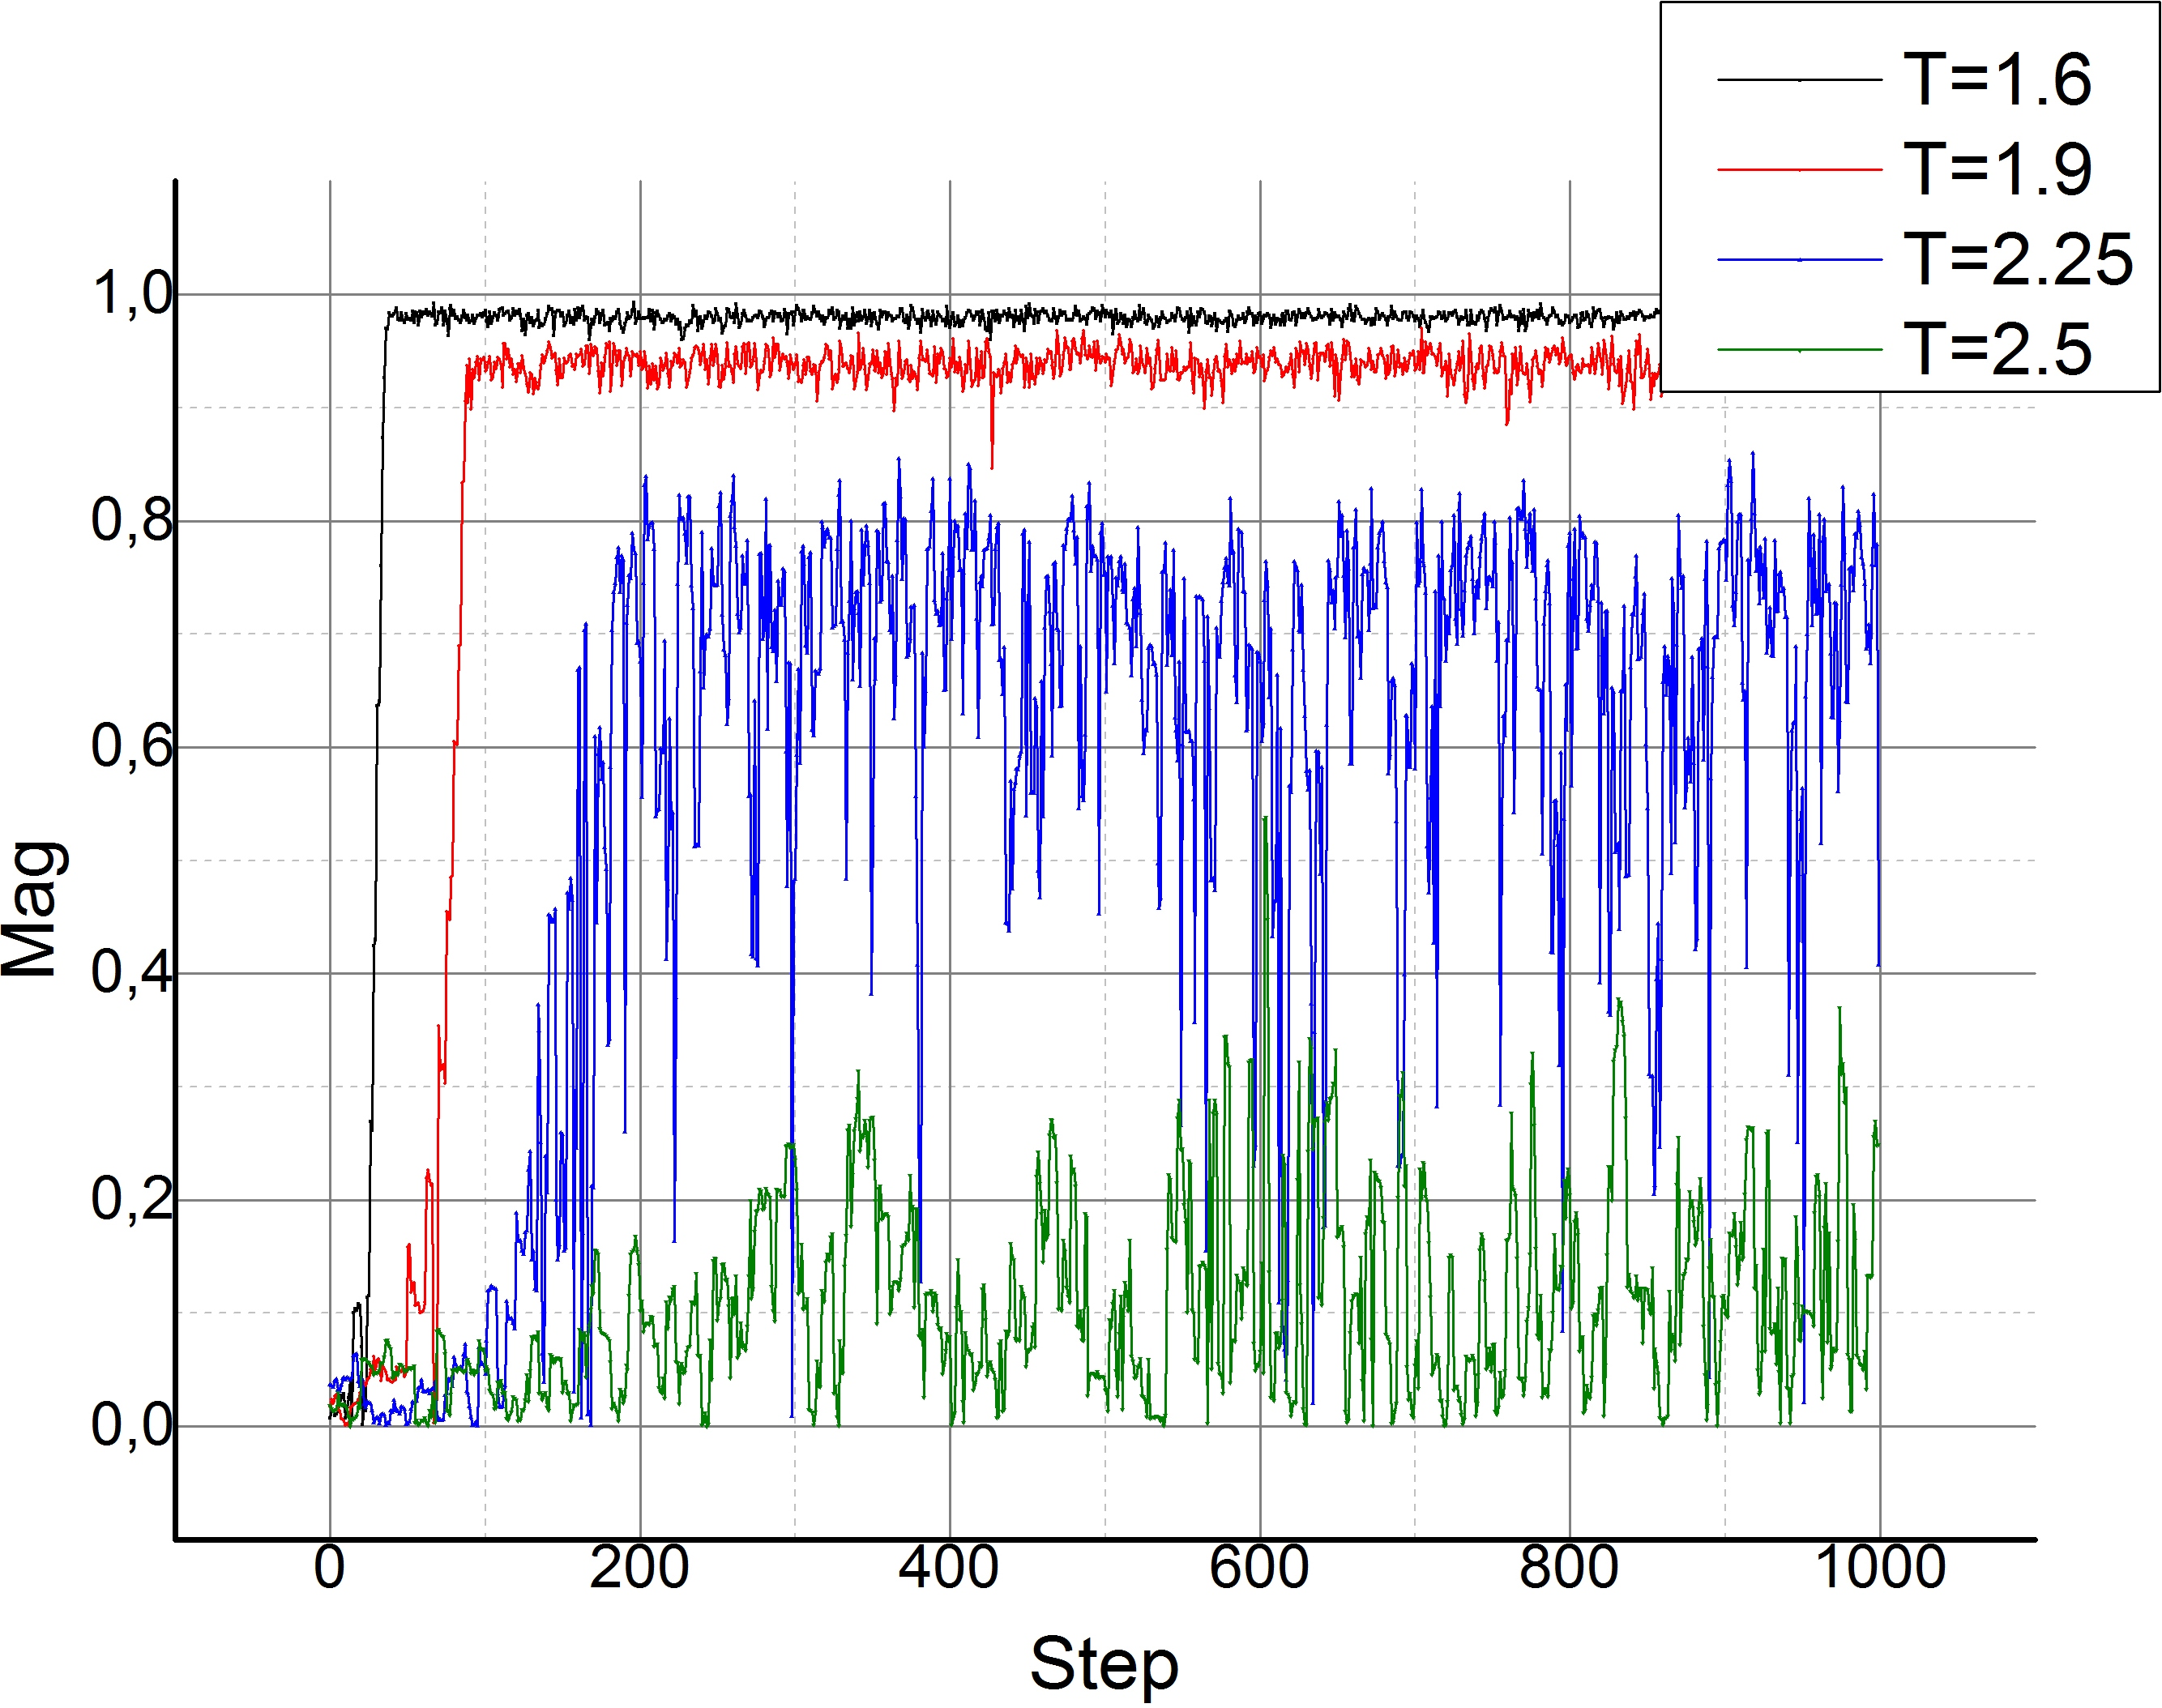
\includegraphics[width=0.30\textwidth]{../Graph_Export/CU2D/abs(m(steps))_Plot.jpg}
	}	
	\subfigure[Konvergenz beim Metropolis-Verfahren]{
		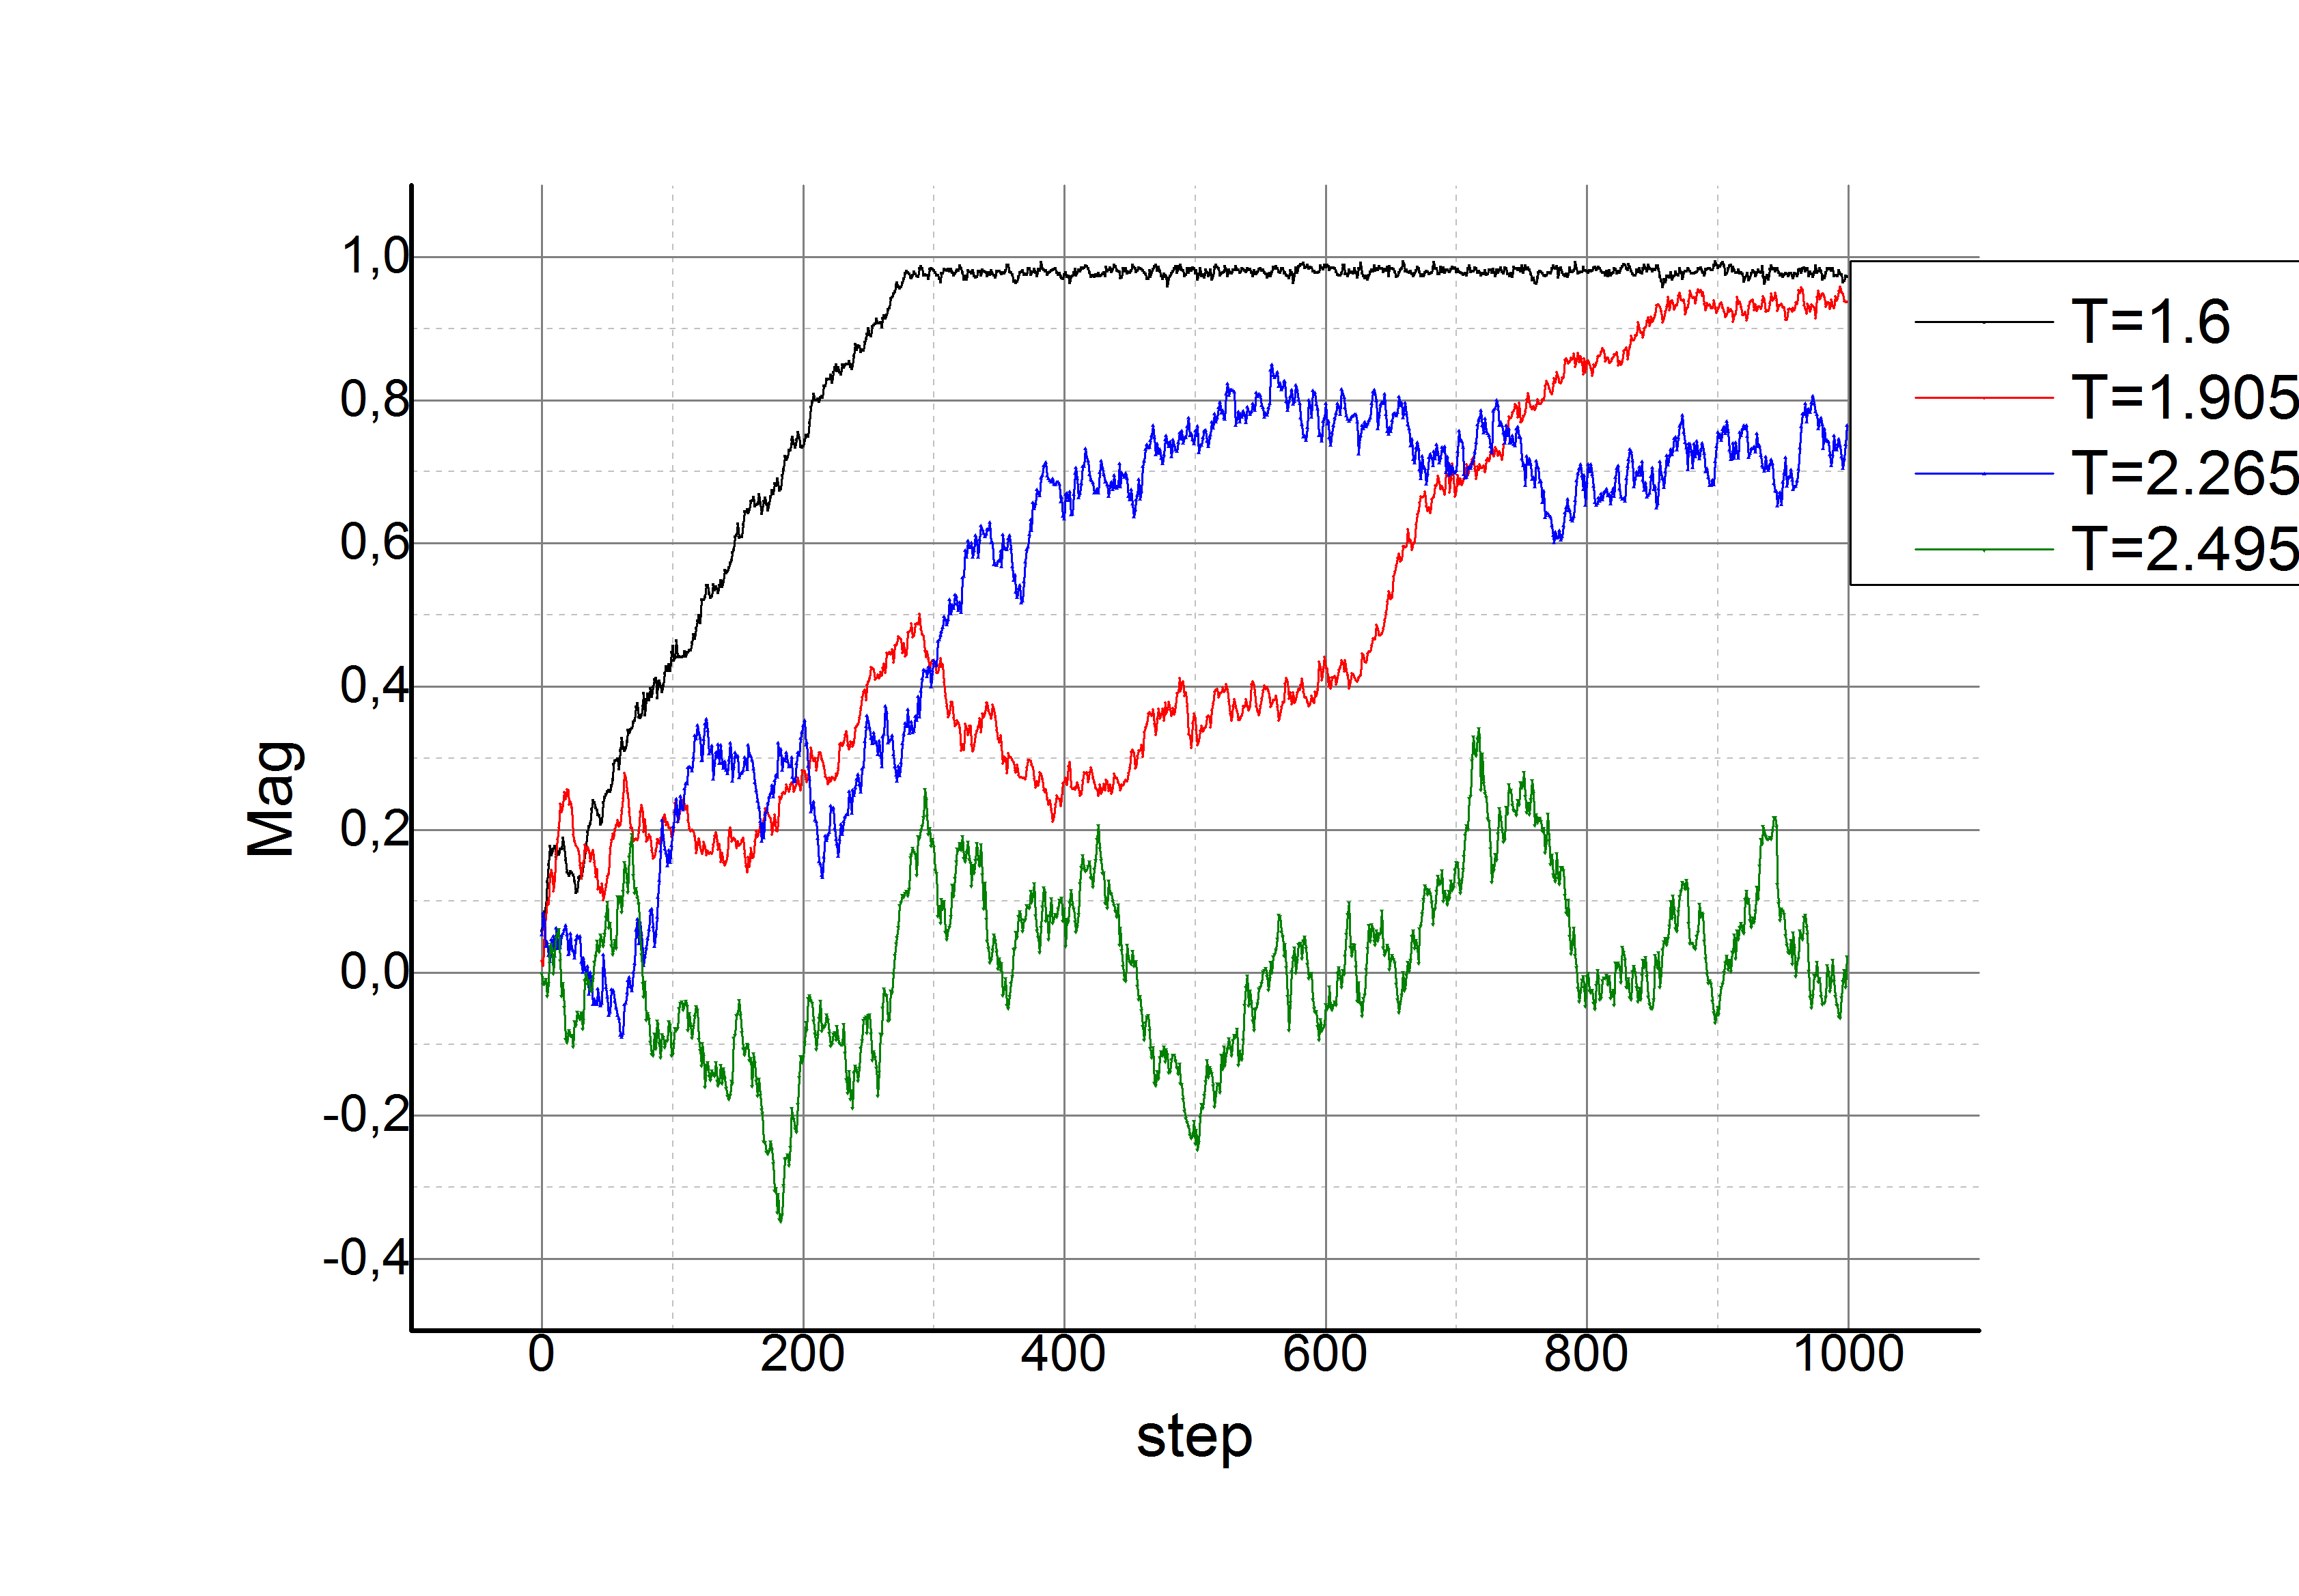
\includegraphics[width=0.30\textwidth]{../Graph_Export/MP2D/m(Steps)_r.jpg}
	}		
	\caption{Konvergenz der Magnetisierung im Vergleich zwischen Metropolis- und Cluster-Update-Verfahren auf einem 50x50 Gitter}
	\label{cu2d2steps}
\end{figure}

Wir erkennen zunächst in Abbildung \ref{cu2d2steps}a, dass es nur Sinn macht, die Betragswerte der Magnetisierung zu betrachten, wenn das Cluster-Update-Verfahren untersucht werden soll. Denn durch das Flippen größerer Cluster springt die Magnetisierung immerzu zwischen negativen und positiven werden.\\
Zu vergleichen sind also sinnvollerweise die Abbildungen \ref{cu2d2steps}b und \ref{cu2d2steps}c. Zunächst ist zu erkennen, dass die Graphen gleicher Temperatur auch gegen die selben Werte konvergieren. Ebenso ist die schnellere Konvergenz des Cluster-Update-Verfahrens deutlich, insbesondere beim Graphen zu $T=1.9$ ist dies schön zu erkennen. Während der Wert beim Metropolis erst nach 800 Schritten gegen 1 konvergiert, tut er dies beim Cluster-Update bereits nach etwa 100. Insofern scheint das Verfahren zu arbeiten, wie erwünscht. Allerdings erzeugt das Cluster-Update sehr stark schwankende Werte für Temperaturen  nahe an Tc oder leicht darüber. Dies liegt wohl daran, dass das Cluster-Update-Verfahren die Instabilität des Systems, die bei diesen Temperaturen vorliegt, stark verdeutlicht, da es global agiert.

\begin{figure}[H]
	\centering
	\subfigure[Konvergenz beim Cluster-Update-Verfahren]{
		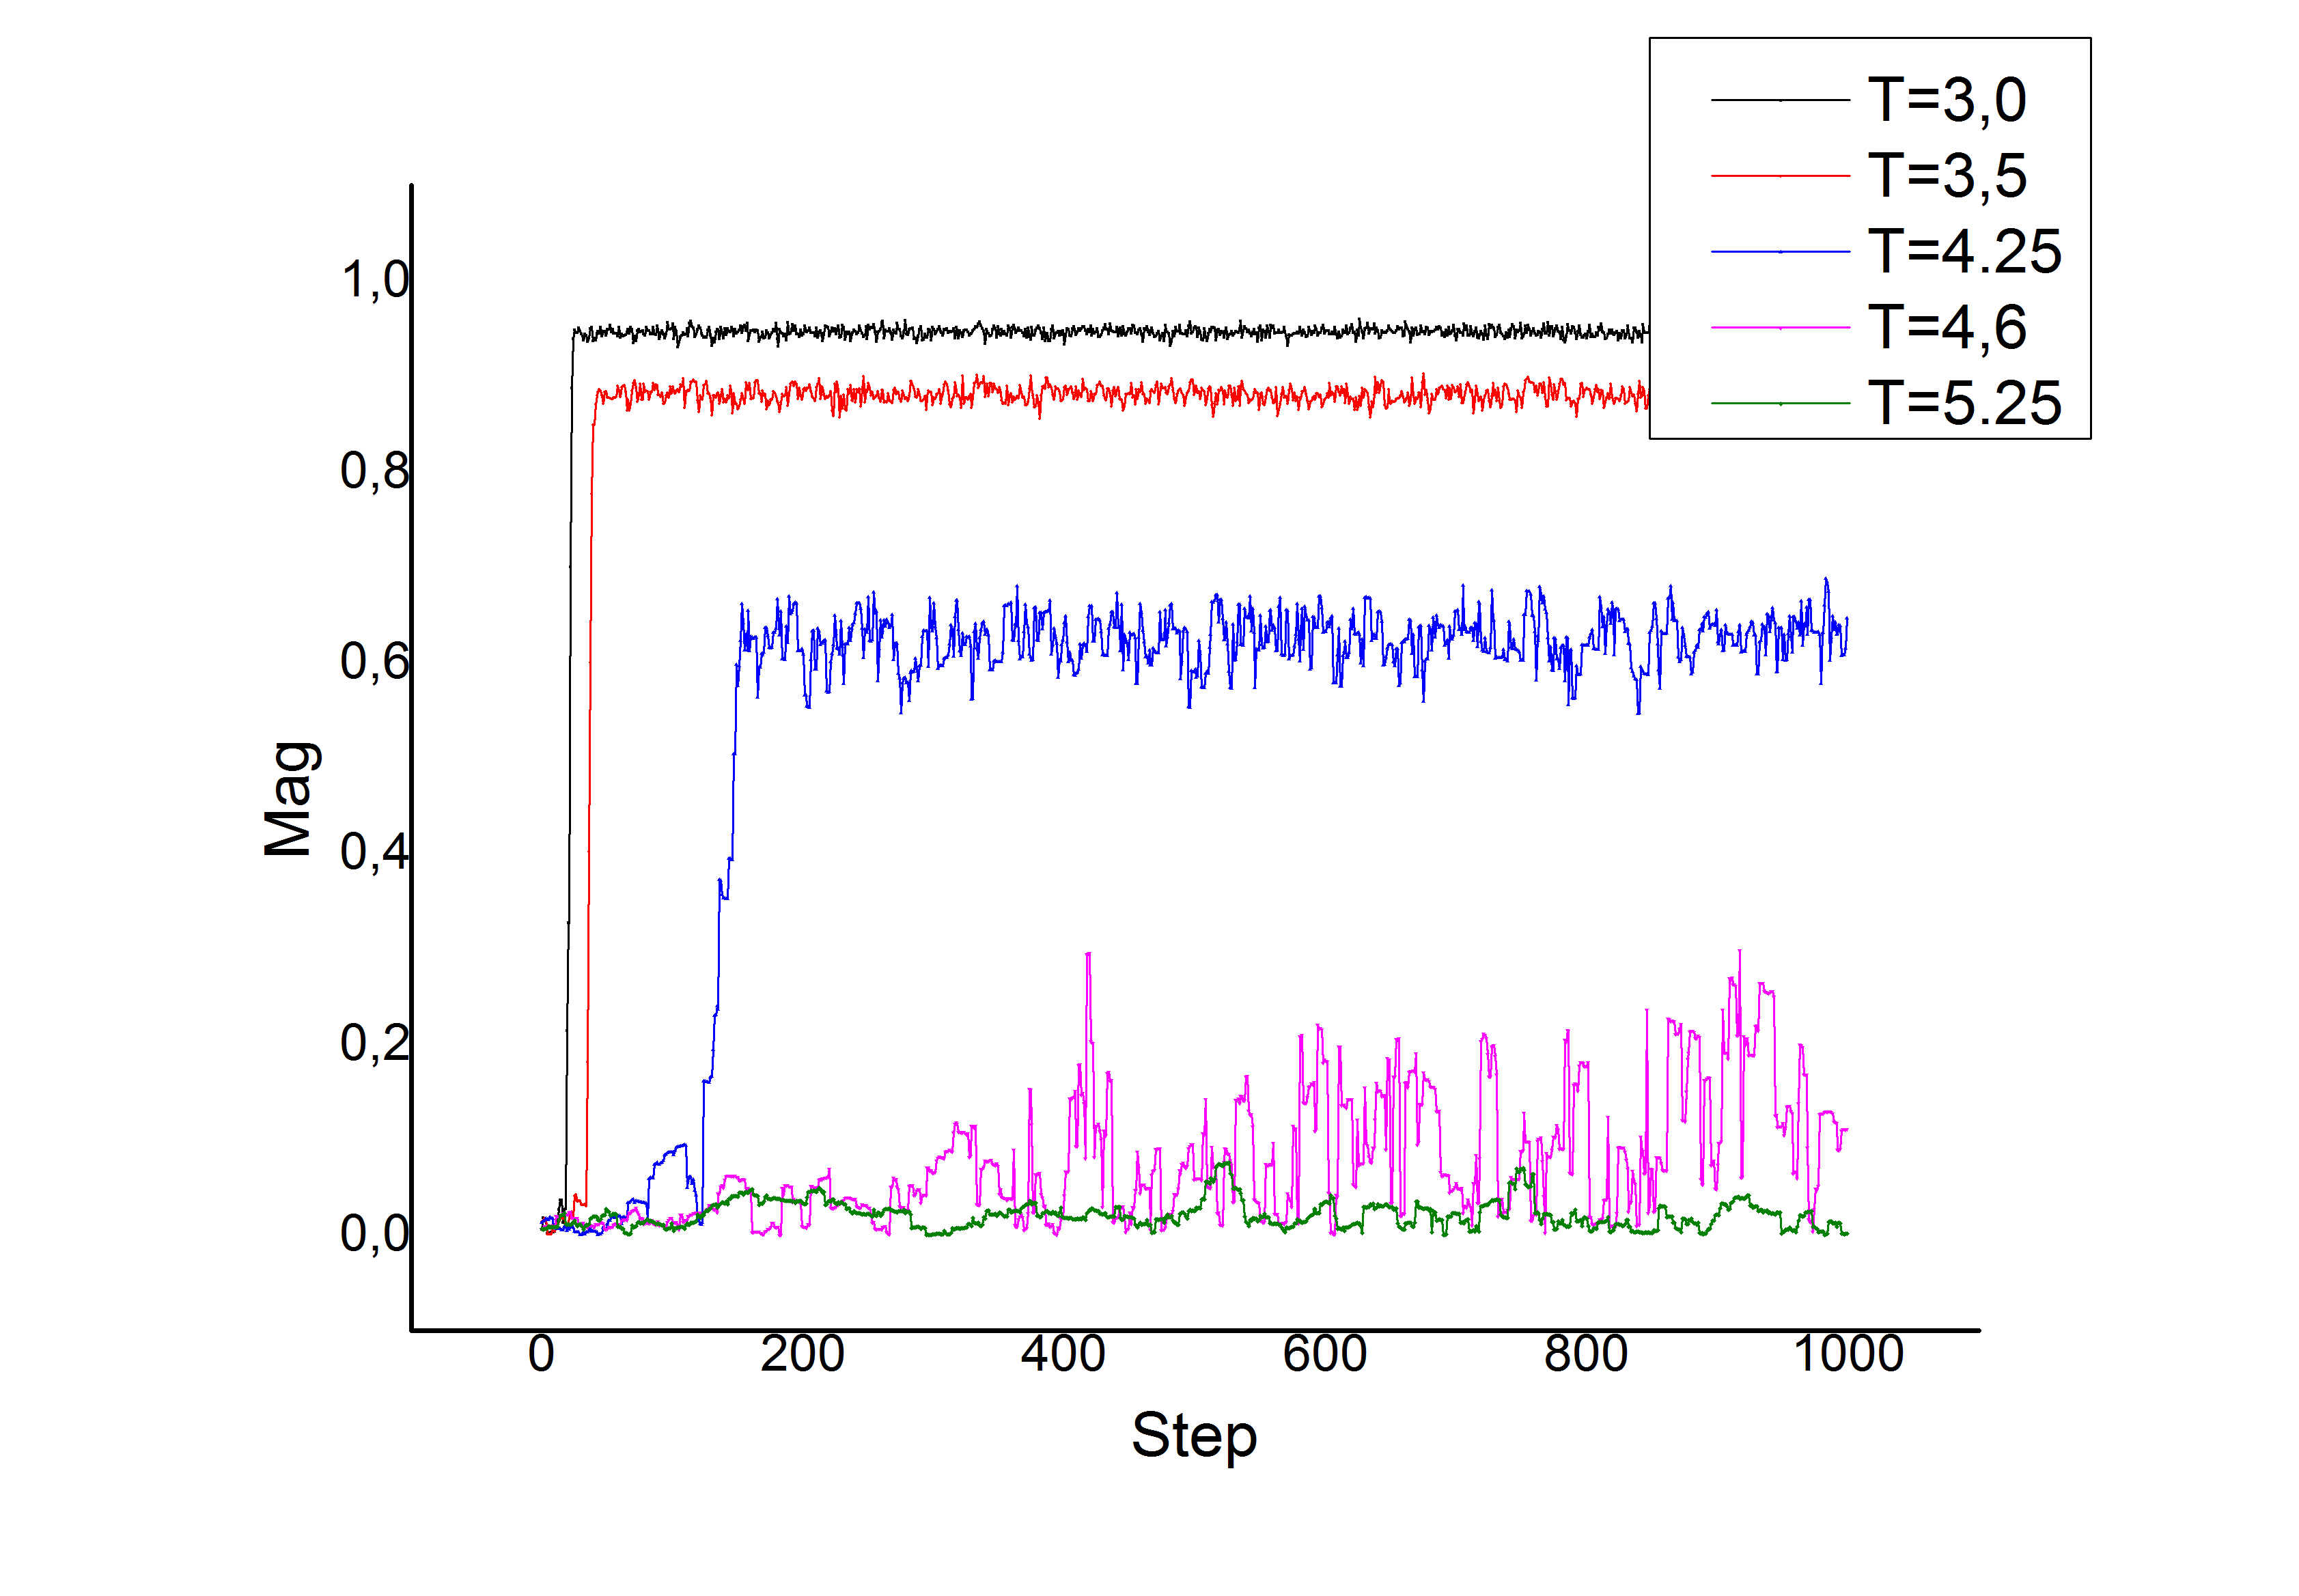
\includegraphics[width=0.47\textwidth]{../Graph_Export/CU3D/abs(m(steps))_Plot.jpg}
	}	
	\subfigure[Konvergenz beim Metropolis-Verfahren]{
		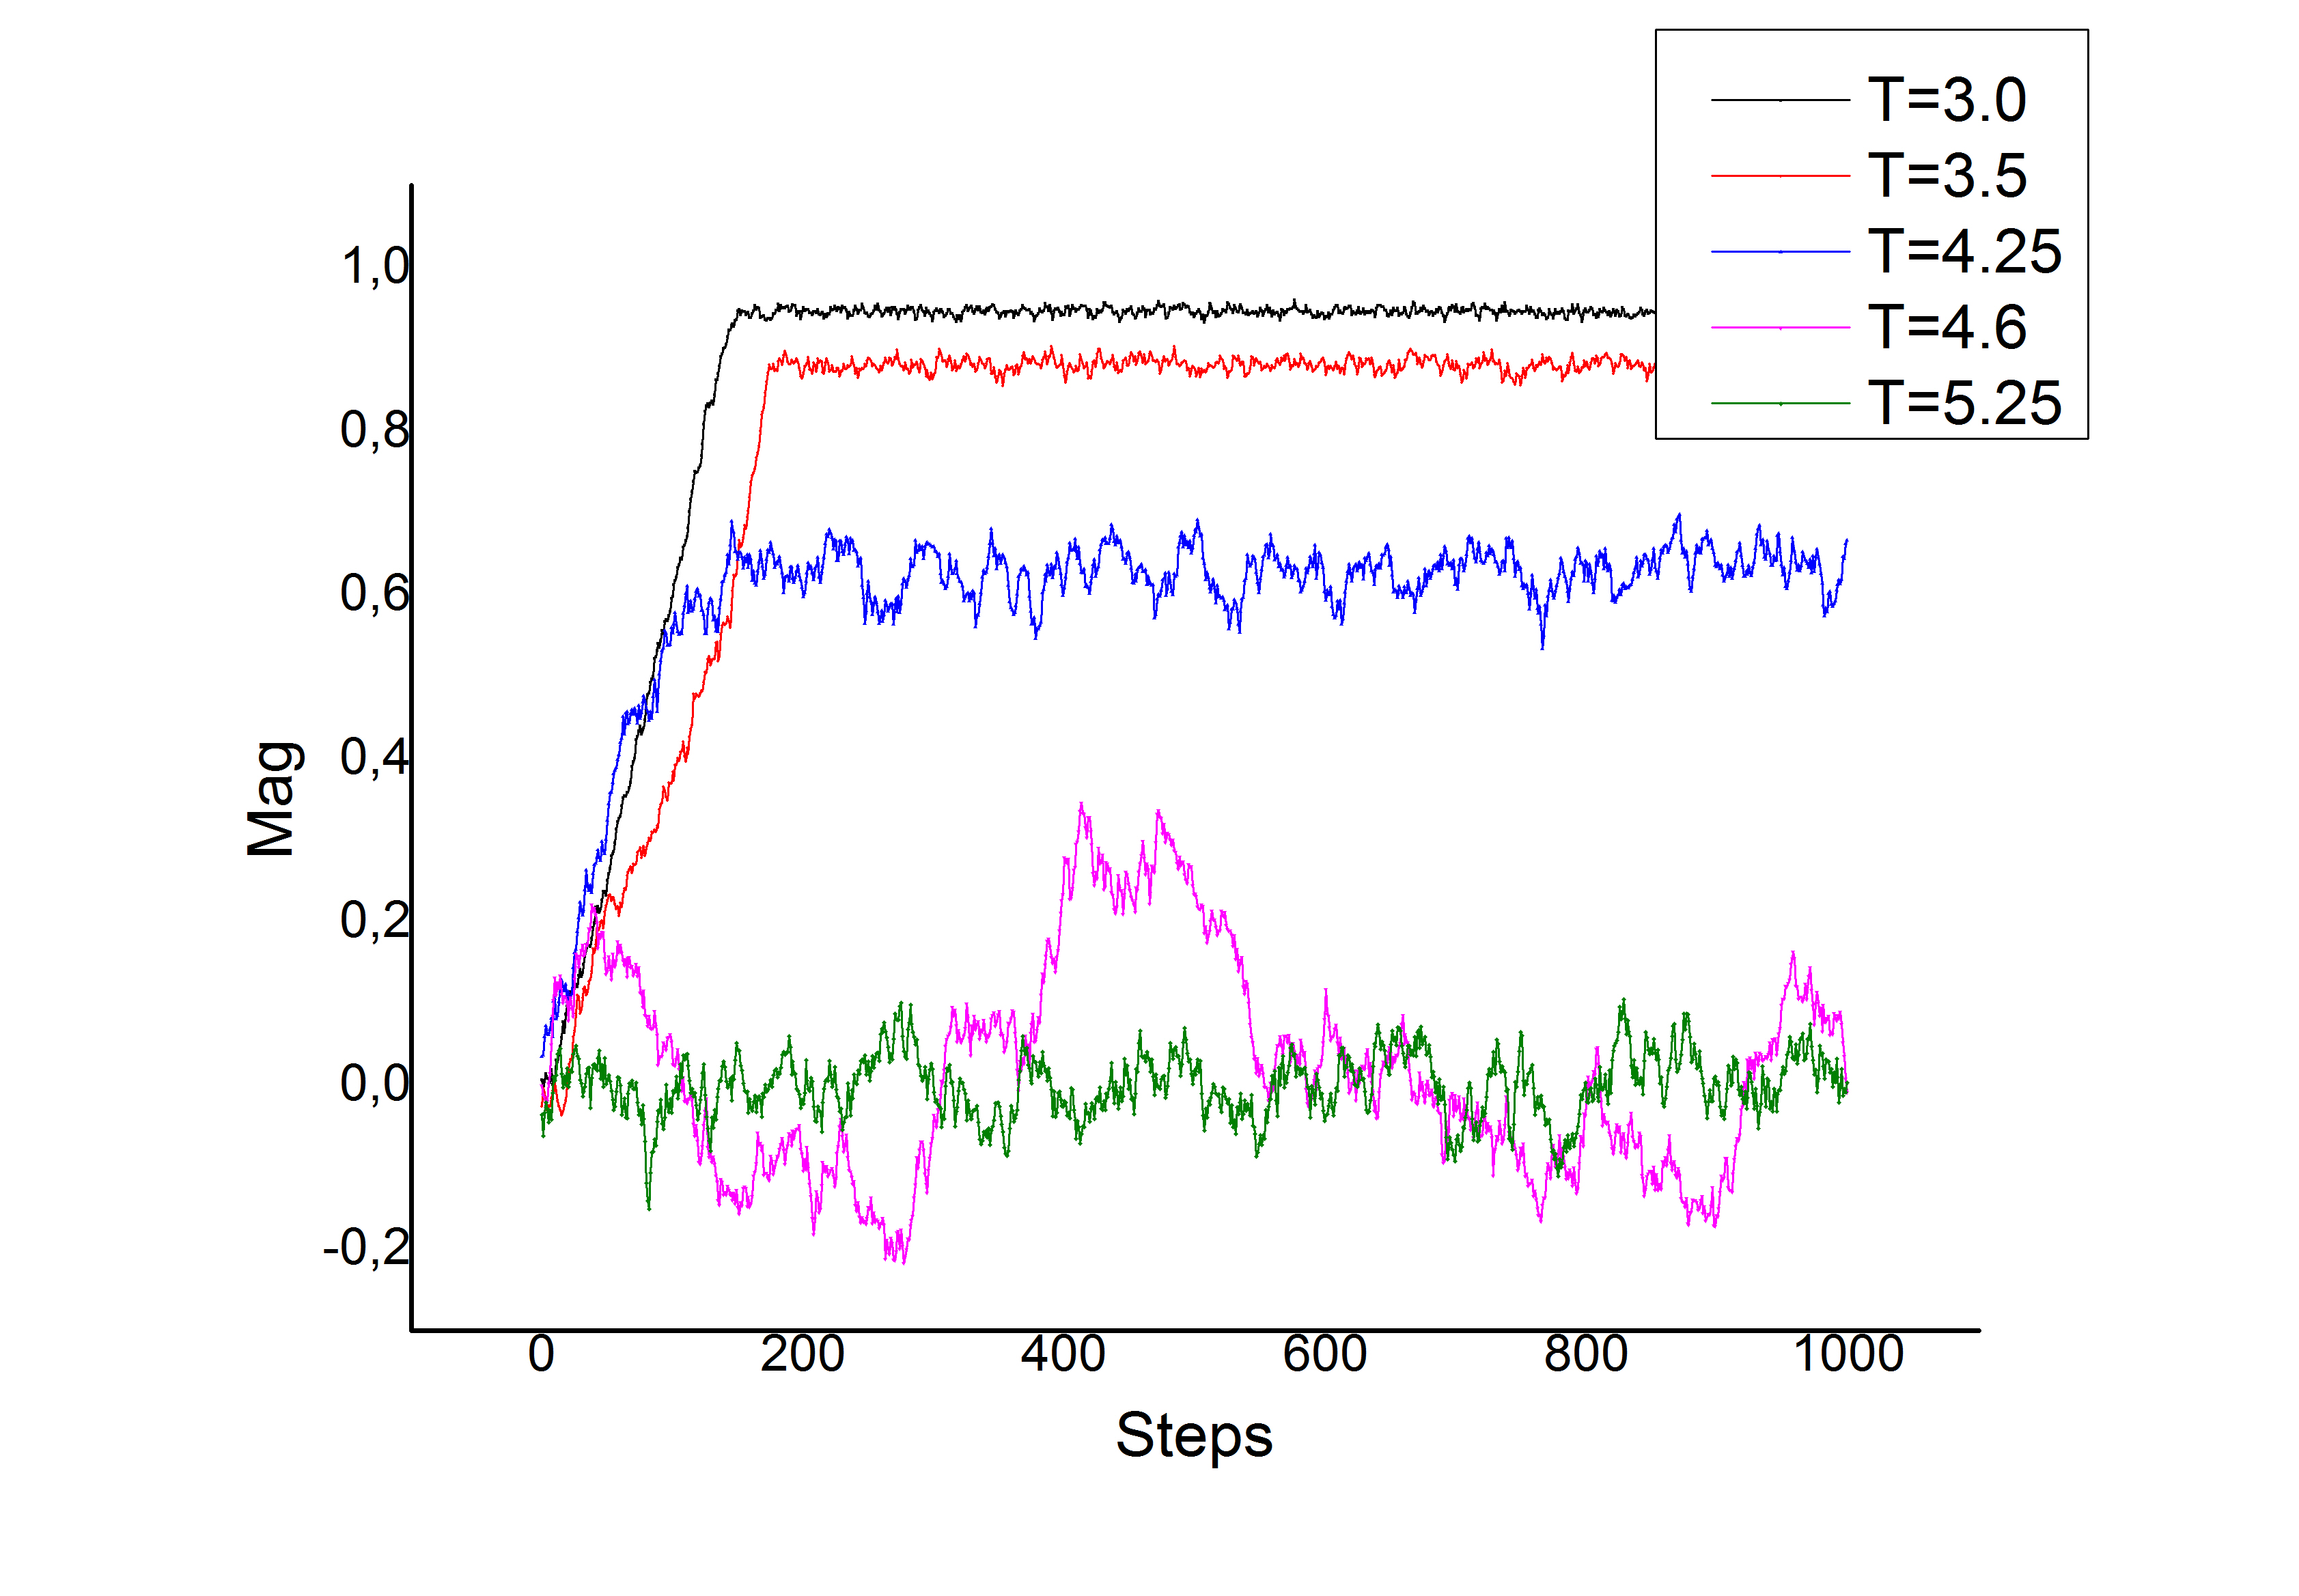
\includegraphics[width=0.47\textwidth]{../Graph_Export/MP3D/m(Steps)_r.jpg}
	}		
	\caption{Konvergenz der Magnetisierung im Vergleich zwischen Metropolis- und Cluster-Update-Verfahren auf einem 20x20x20 Gitter}
	\label{cu2d3steps}
\end{figure}

Bei der Simulation auf einem dreidimensionalen Gitter erkennt man die gleichen Phänomene, wie beim Zweidimensionalen. Die Konvergenz ist insgesamt etwas schneller.

\begin{figure}[H]
	\centering
	\subfigure[Cluster-Update-Verfahren]{
		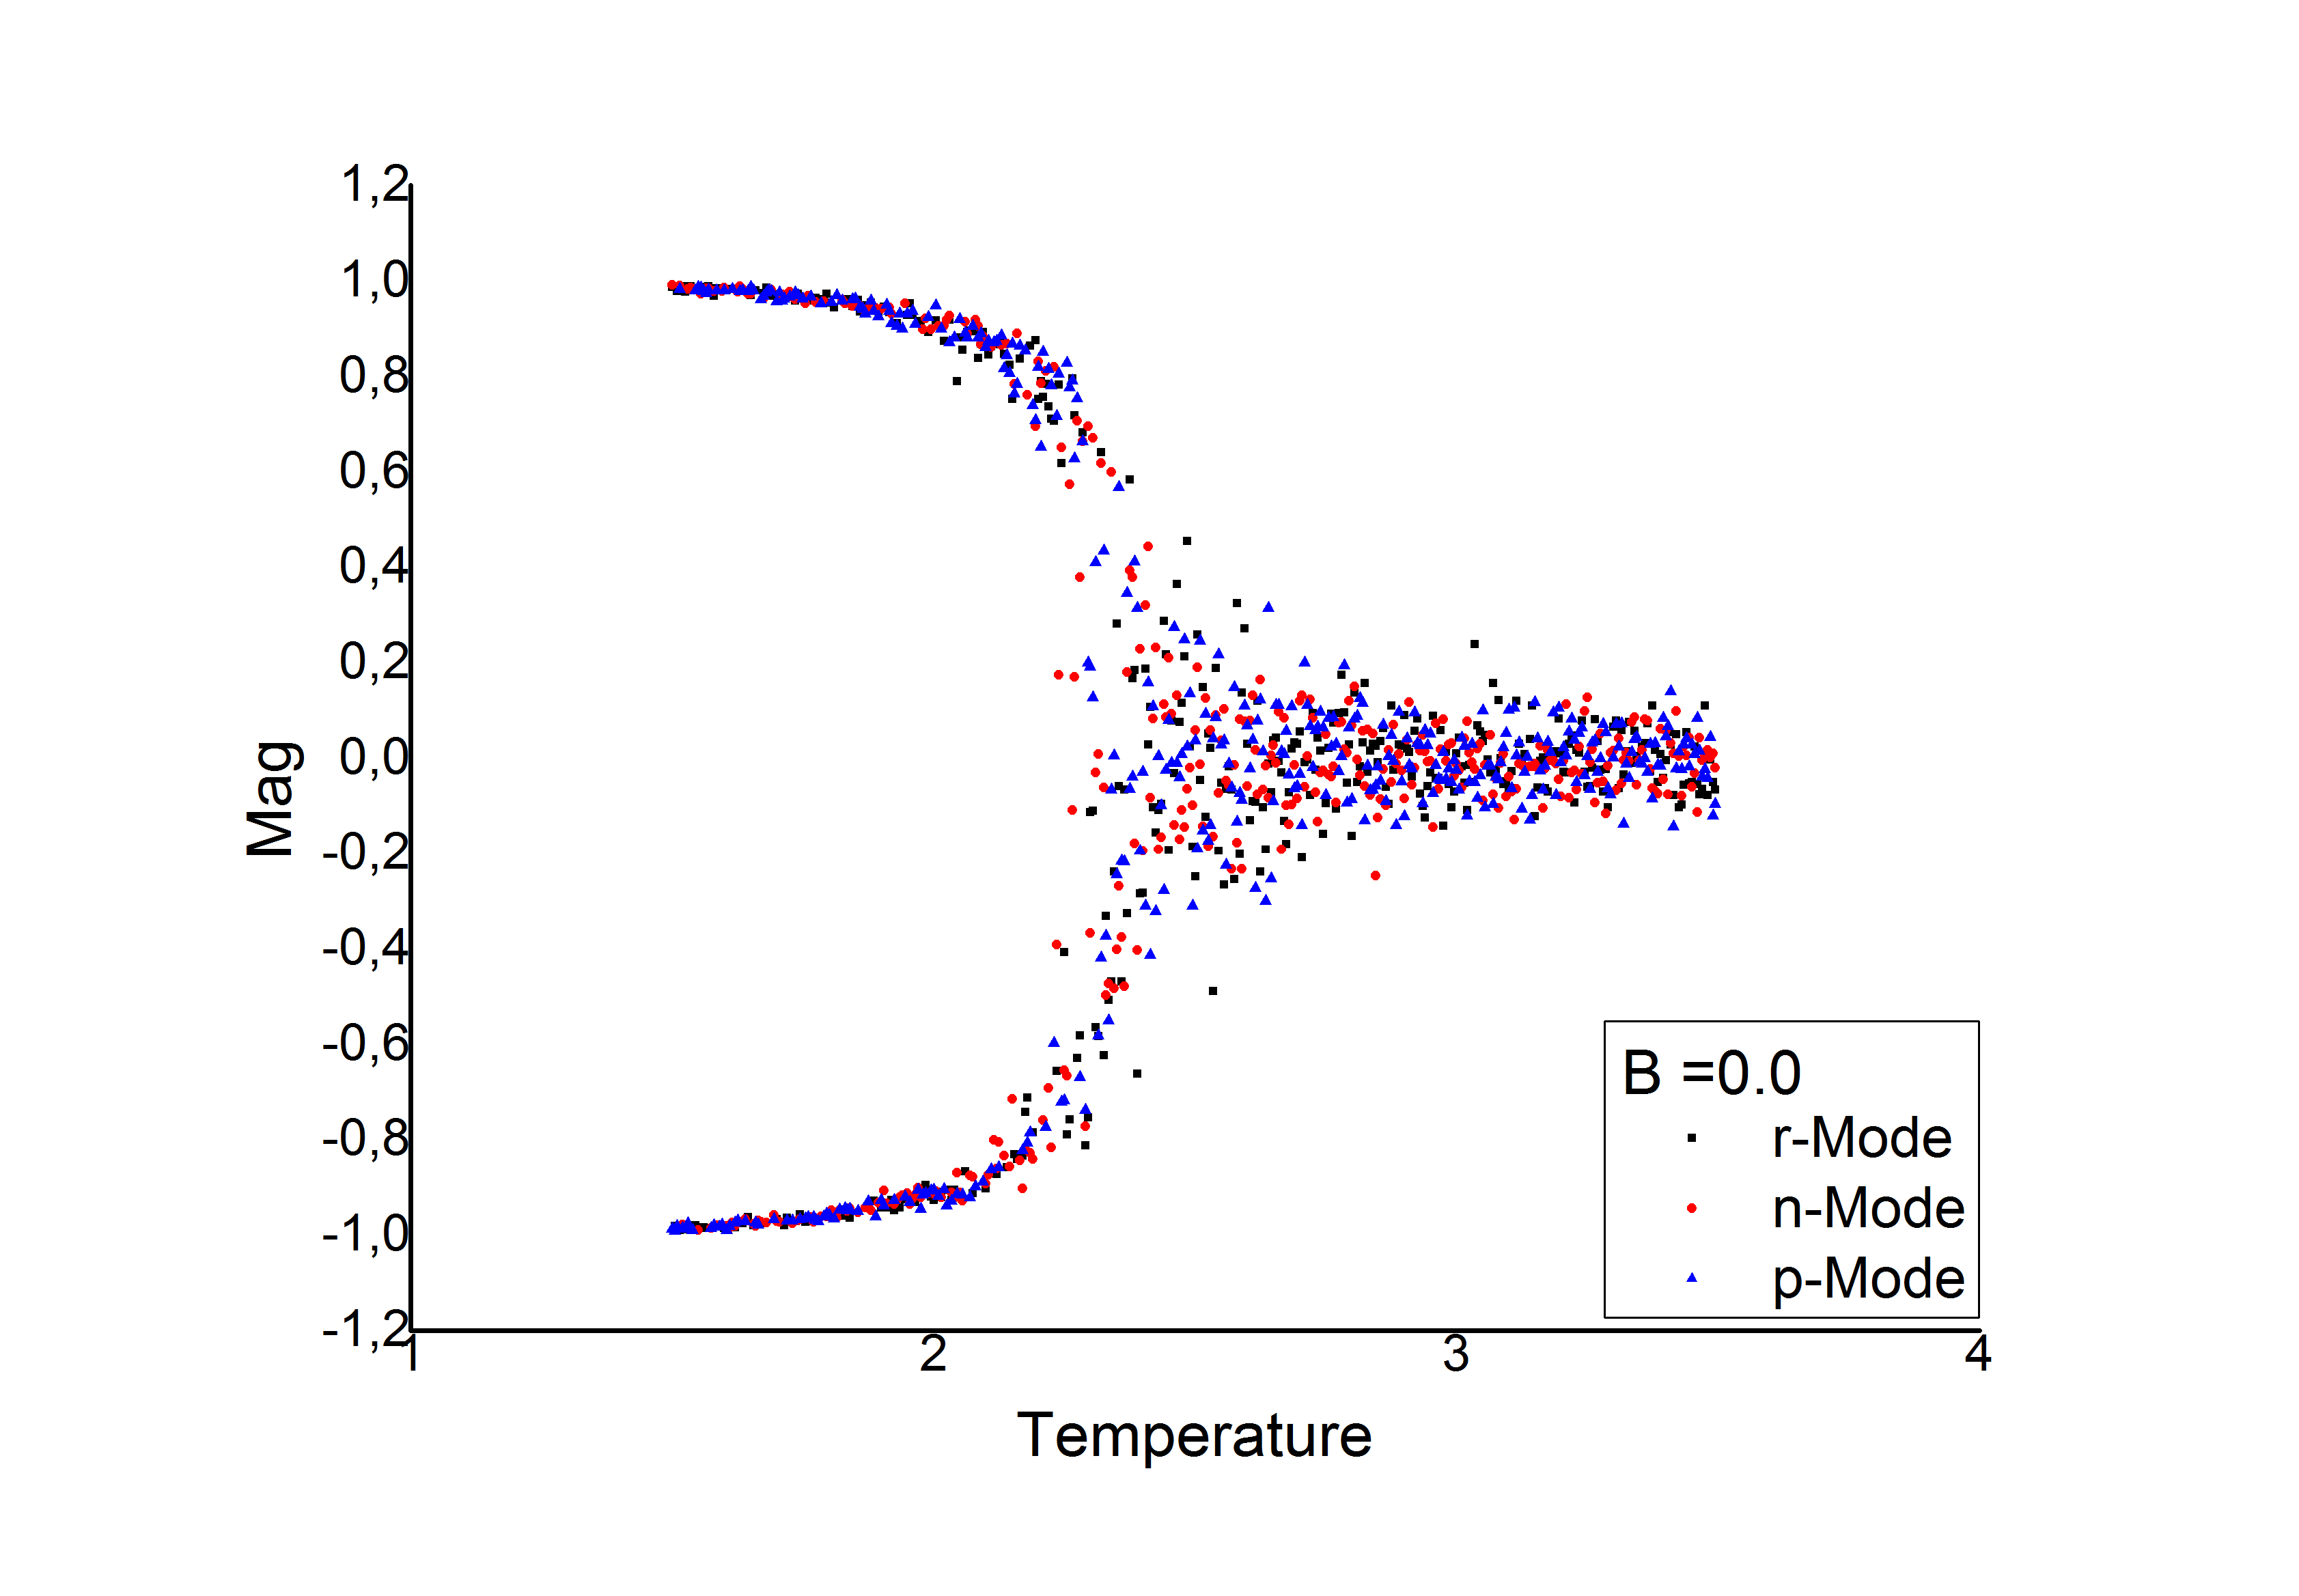
\includegraphics[width=0.47\textwidth]{../Graph_Export/CU2D/m(T)_B=0_matModes_CU2D_Plot.jpg}
	}
	\subfigure[Metropolis-Verfahren]{
		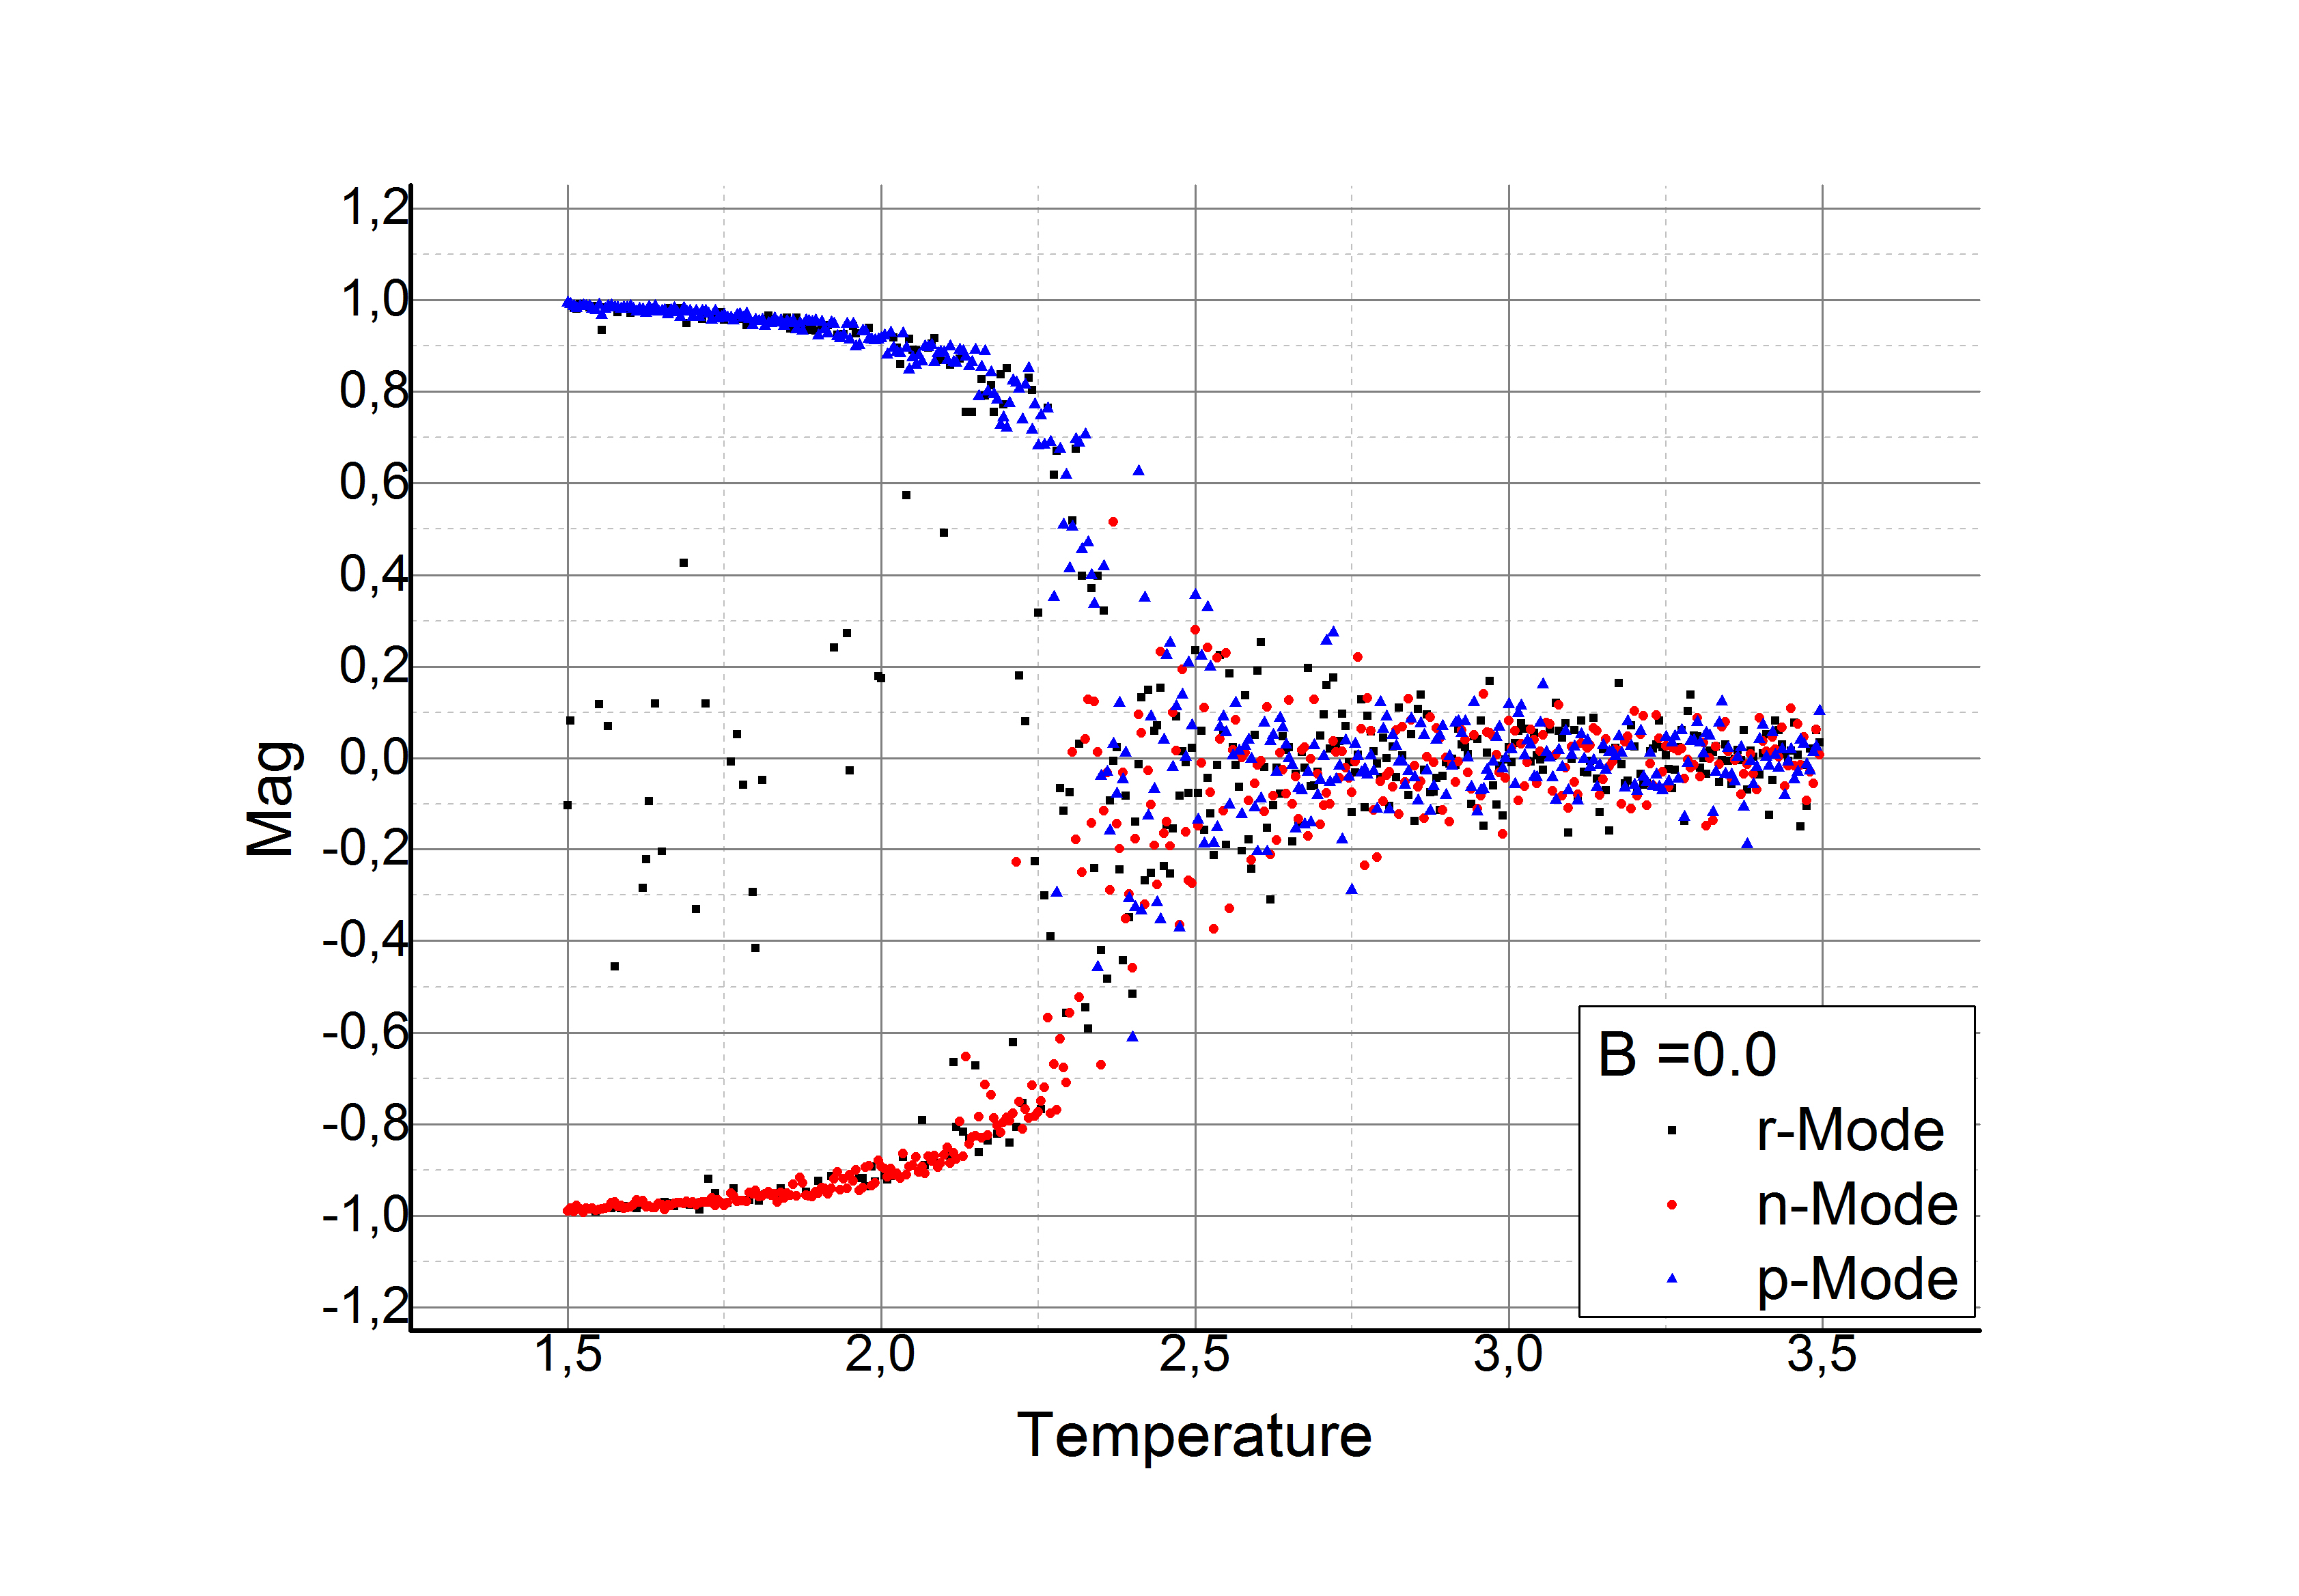
\includegraphics[width=0.47\textwidth]{../Graph_Export/MP2D/m(T)_B=0_matModes_MP2D_50_Plot.jpg}
	}		
	\caption{Temperaturabhängigkeit der Magnetisierung auf einem 50x50 Gitter}
	\label{}
\end{figure}

Die Temperaturabhängigkeit unterscheidet sich nur im Detail. So gibt es keine Ausreißer mehr, im Bereich zwischen 1.5 und 2.2. Zustände, die den lokalen Metropolis bisher verklemmt haben, werden durch den globalen Ansatz unschädlich gemacht. 

\newpage
\section{Zusammenfassung}
Hier könnte dein Fazit stehen... :)\\
Die Monte-Carlo-Methode mit Metropolis-Algorithmus ist eine simple Möglichkeit, das Ising-Modell zu simulieren und führt zumindest im 2-dimensionalen schnell zu anschaulichen Ergebnissen. So erhalten wir eine kritische Temperatur $ T_c \approx 2.26 $ (analytisch: $\approx 2.2692$) Im 3-dimensionalen, wo es keine analytische Lösung gibt, ist die Rechenzeit deutlich erhöht, aber immer noch vertretbar.\\
Außerdem lässt sich der Einfluss eines äußeren Magnetfeldes studieren, während man aber bereit sein muss, eine gewisse Anzahl an Rechenschritten am Anfang zu ignorieren, bis das System konvergiert ist. Des Weiteren kommt es noch nach der Konvergenz zu einem relativ breiten Rauschen um den erreichten Wert.\\
Die Untersuchung des Cluster-Update-Verfahrens durch den Einsatz des Wolff-Algorithmus hat gezeigt, dass dieser sowohl Vor- als auch Nachteile bietet.\\
Als Vorteil ist sicherlich die schnellere Konvergenz zu erwähnen, durch die massiv Rechenzeit eingespart werden könnte. Zudem wird der "critical-slowdown" den ein lokales Verfahren mit sich bringt verhindert.\\
Das Cluster-Update ist allerdings nicht brauchbar, wenn der exakte Verlauf der Magnetisierung untersucht werden soll, da man die Absolutwerte der Messergebnisse betrachten muss. Zudem ist die Einwirkung eines externen Magnetfeldes nicht sinnvoll untersuchbar.
 

\newpage
\listoffigures

\

\

Alle Abbildungen ohne Quellenangabe sind in Eigenproduktion erstellt.


\section*{Quellen}
\begin{itemize}
\item http://www.theorie.physik.uni-goettingen.de/~honecker/bs/semstat/ausarb/schart.pdf
\item http://www.tat.physik.uni-tuebingen.de/~kley/lehre/cp-prakt/projekte/projekt2.pdf
\item http://www.tat.physik.uni-tuebingen.de/~kley/lehre/cp-prakt/projekte/projekt-judd.pdf
\item http://pauli.uni-muenster.de/Seminare/teilchen/teilchen\_ws05/Ising.pdf
\item K. Binder, D. W. Heermann, Monte Carlo Simulation in Statistical Physics, Springer, 2010
\item M. Troyer, Magnetic models and phase transitions, ETH Zürich, 2011\\\\
Cluster-Algorithmen:
\item http://www.icp.uni-stuttgart.de/~icp/mediawiki/images/0/03/Hs0910\_thass\_ausarbeitung.pdf
\item http://www.netlib.org/utk/lsi/pcwLSI/text/node292.html
\item http://katzgraber.org/teaching/ss07/files/andrist.pdf
\end{itemize}
\newpage
\end{document}
